\documentclass[a4paper,11pt,spanish, twoside, leqno]{tfg-uam}

\usepackage[utf8]{inputenc}
\usepackage{amsfonts, amssymb, amsmath, amsthm}
\usepackage{graphicx}
\usepackage{color}

\newcommand*{\reales}{\mathbb{R}}
\newtheorem{teor}{Teorema}[chapter]
\newtheorem{lema}[teor]{Lema}
\newtheorem{corolario}[teor]{Corolario}
\newtheorem*{teorsin}{Teorema}
\newtheorem*{corolariosin}{Corolario}


\theoremstyle{definition}
\newtheorem{defin}[teor]{Definici\'on}

\title{Teorema de clasificación de superficies}
\author{Rodrigo De Pool}
\tutor{Javier Aramayona}
\curso{2019-2020}


%%%%%METADATOS: rellenar la info solicitada entre llaves
\usepackage{hyperref}
\hypersetup{
	pdfinfo={
            Title={Teorema de clasificaci\'on de superficies }, %Titulo del trabajo; ejemplo: Matematicas y desarrollo
            Author={ Rodrigo De Pool}, %Autor del trabajo; ejemplo: Juan Sanchez
            Director1={javier.aramayona }, %Tutor1: en formato nombre.apellido, tal como aparece en la primera parte, antes de la arroba,  de su direcci�n de correo electr�nico de la UAM; ejemplo: fernando.soria
            Director2={ }, %Tutor2: en formato nombre.apellido, tal como aparece en la primera parte, antes de la arroba,  de su direcci�n de correo electr�nico de la UAM
            Ndirectores={1 }, %Numero total de directores: 1 � 2
            Tipo={TFG}, %no tocar
            Curso={2018-19}, %no tocar
            Palabrasclave={ },% Palabras clave del trabajo, separadas por comas y sin acentos ni espacios; ejemplo: morfismos, formas modulares, ecuaciones elipticas
				}
}
%%%%%%%%%%%%%%%%%%%%%%%%%%%%%%%

\begin{document}





\begin{abstract}[spanish]

El trabajo comprende un estudio riguroso de las superficies topológicas y su clasificación:

El primer bloque inicia introduciendo las nociones elementales de superficies compactas y procede a demostrar que, bajo hipótesis de compacidad, toda superficie es topológicamente equivalente: o a una esfera, o a una suma conexa finita de toros, o a una suma conexa finita de planos proyectivos. 

Posteriormente, estudiaremos el resultado Keréjártó, que generaliza la clasificación retirando la exigencia de compacidad. En esta nueva incursión hará falta definir el concepto de `frontera ideal', un invariante topológico que describe cómo subsuperficies compactas dividen a la superficie en cuestión. Demostraremos que, fijado el `género' y la `clase de orientabilidad', una superficie viene determinada topológicamente por su frontera ideal. 

Luego, daremos representantes para las clases de equivalencia de la clasificación no compacta. Utilizando un resultado topológico veremos que toda frontera ideal es homeomorfa a un subconjunto del conjunto de Cantor. Más aún, estudiaremos una especie de recíproco descrito por Ian Richards en \cite{ian}: Dado un subconjunto cualquiera del conjunto de Cantor construiremos una superficie que lo tiene por frontera ideal. Esta construcción nos permitirá dar el representante para cada clase de equivalencia. Finalmente, haremos un breve apunte sobre la numerabilidad de las superficies homeomorfas según las hipótesis de la clasificación.
\end{abstract}

\begin{abstract}[english]
This essay contains a mathematical approach to topological surfaces and their classification:

Firstly, basic notions of compact surfaces will be introduced, from which a proof of their classification will be given. As a result we will find that any compact surface is homeomorphic either to: a sphere, or a  finite \textit{connected sum} of torus, or a finite \textit{connected sum} of projective planes.

Afterwards, we will proceed to study the Kerékjártó's theorem, the classification without the hypothesis of compactness. For this, we will require to introduce the concept of ideal boundary, a topological invariant that describes how a surface is divided by its compact subsurfaces. The theorem will guarantee that, with a `genus' and `orientability class', a surface will be topologically determined by its ideal boundary.

Furthermore, we will give a representative for each equivalence class of the classification. A topological result will prove that any ideal boundary is homeomorphic to a subset of the Cantor set. Evenmore, a construction by Ian Richards will prove that given any subset of the Cantor set one can construct a surface that has it as ideal boundary. This construction will allows us to present such representatives. Lastly, we will briefly discuss the numerability of homeomorphic surfaces.
\end{abstract}





\mainmatter
\chapter{Introducción}
En este capítulo introduciremos la noción de superficie topológica de manera rigurosa. Además, nos familiarizaremos con los conceptos de suma conexa y triangulación, componiendo ambas las herramientas esenciales para probar la clasificación de superficies compactas.
\section{Introducci\'on a las superficies topológicas}
El concepto de superficie topológica busca generalizar la idea de \textit{superficie} en el sentido usual. Más concretamente, buscamos abarcar todo conjunto que comparta localmente las propiedades topológicas de una superficie en $\mathbb{R}^n$. 

\begin{defin}
\label{defin:superficie}
Diremos que un espacio topológico, $S$, es una \textbf{superficie topológica} si para todos sus puntos existe un entorno homeomorfo a $U^2 = \{x\in \mathbb{R}^2: ||x||<1 \}$. Además, a $S$ se le exige ser Hausdorff, segundo numerable y conexo. \footnote{Si retiramos la hipótesis de conexión y sustituimos $U^2$ por $U^n$, obtenemos una \textbf{n-variedad} topológica. Sin embargo, en este trabajo nos limitamos al estudio de las 2-variedades conexas (superficies).}
\end{defin}
Consideremos los siguientes ejemplos de superficies topológicas:
\begin{enumerate}
\item El conjunto $ U^2 = \{ x\in\mathbb{R}^2: ||x||<1 \} $, dotado de la topología de subespacio, es una superficie. 

\item El cuadrado sin bordes
\[ C = \{(x,y)\in \mathbb{R}^2: 0 <  x < 1,\, 0 < y < 1 \} \]
al ser dotado de la topología de subespacio, también es ejemplo de superficie.

\item Dado un homeomorfismo cualquiera:
\[ f:S \rightarrow X \]
tendremos que si $S$ es una superficie topológica, entonces $f(S)$ también lo es.
\end{enumerate}

Por otro lado, si consideramos el cuadrado con sus bordes ($\overline{C}$), el conjunto no compone un ejemplo de superficie tal y como lo definimos. En este conjunto los puntos que pertenecen a las aristas no tienen entornos homeomorfos a $U^2$. Veremos que $\overline{C}$ es una \textquoteleft superficie con borde \textquoteright, concepto que estudiaremos más adelante (véase la sección \ref{sec:superfborde}).
\subsection{Orientación de superficies}
\label{sec:orientabilidad}
Las superficies se dividen en dos clases: Las orientables y las no orientables. En este trabajo no ahondaremos con formalidad matemática en este concepto, asumiremos que a las superficies tratadas pueden dotarse de una estructura diferencial y con ello podemos recurrir a la noción de orientabilidad estudiada en el grado. Sin embargo, bastaría con extender el concepto de orientabilidad para que los resultados aquí propuestos valieran para cualquier superficie topológica.

El principal resultado que usaremos al respecto es que la orientabilidad es una propiedad topológica (se conserva por homeomorfismos). En el contexto del teorema de clasificación de superficies, observaremos como la orientabilidad de la superficie nos delimitará las clases de equivalencia a las que una superficie puede pertenecer.

\section{Superficies compactas}

En nuestro objetivo de acercarnos a una clasificación  completa de superficies, empezaremos por estudiar el caso de las superficies compactas. Para ello necesitaremos primero hacernos con un bagaje de ejemplos de superficies compactas elementales. Sin más preámbulo, alimentemos la curiosidad del lector con estos suculentos ejemplos:

\subsection*{La esfera}
El conjunto $ \mathbb{S}^2 = \{x\in \mathbb{R}^3: ||x||=1 \} $ conforma un ejemplo de superficie compacta. Alternativamente, se puede expresar la esfera como el disco $ D = \{(x,y)\in\mathbb{R}^2: ||(x,y)||\leq1 \} $, realizando la identificación  \ref{esferaid} y dotando al conjunto resultante de la topología cociente.
\begin{align}\label{esferaid}
	(x,y)\equiv(x,-y),\quad\forall(x,y)\in fr(D)
\end{align}
Se puede comprobar que ambas formas de definir la esfera son homeomorfas. 

\begin{figure}[h!]
	\centering
	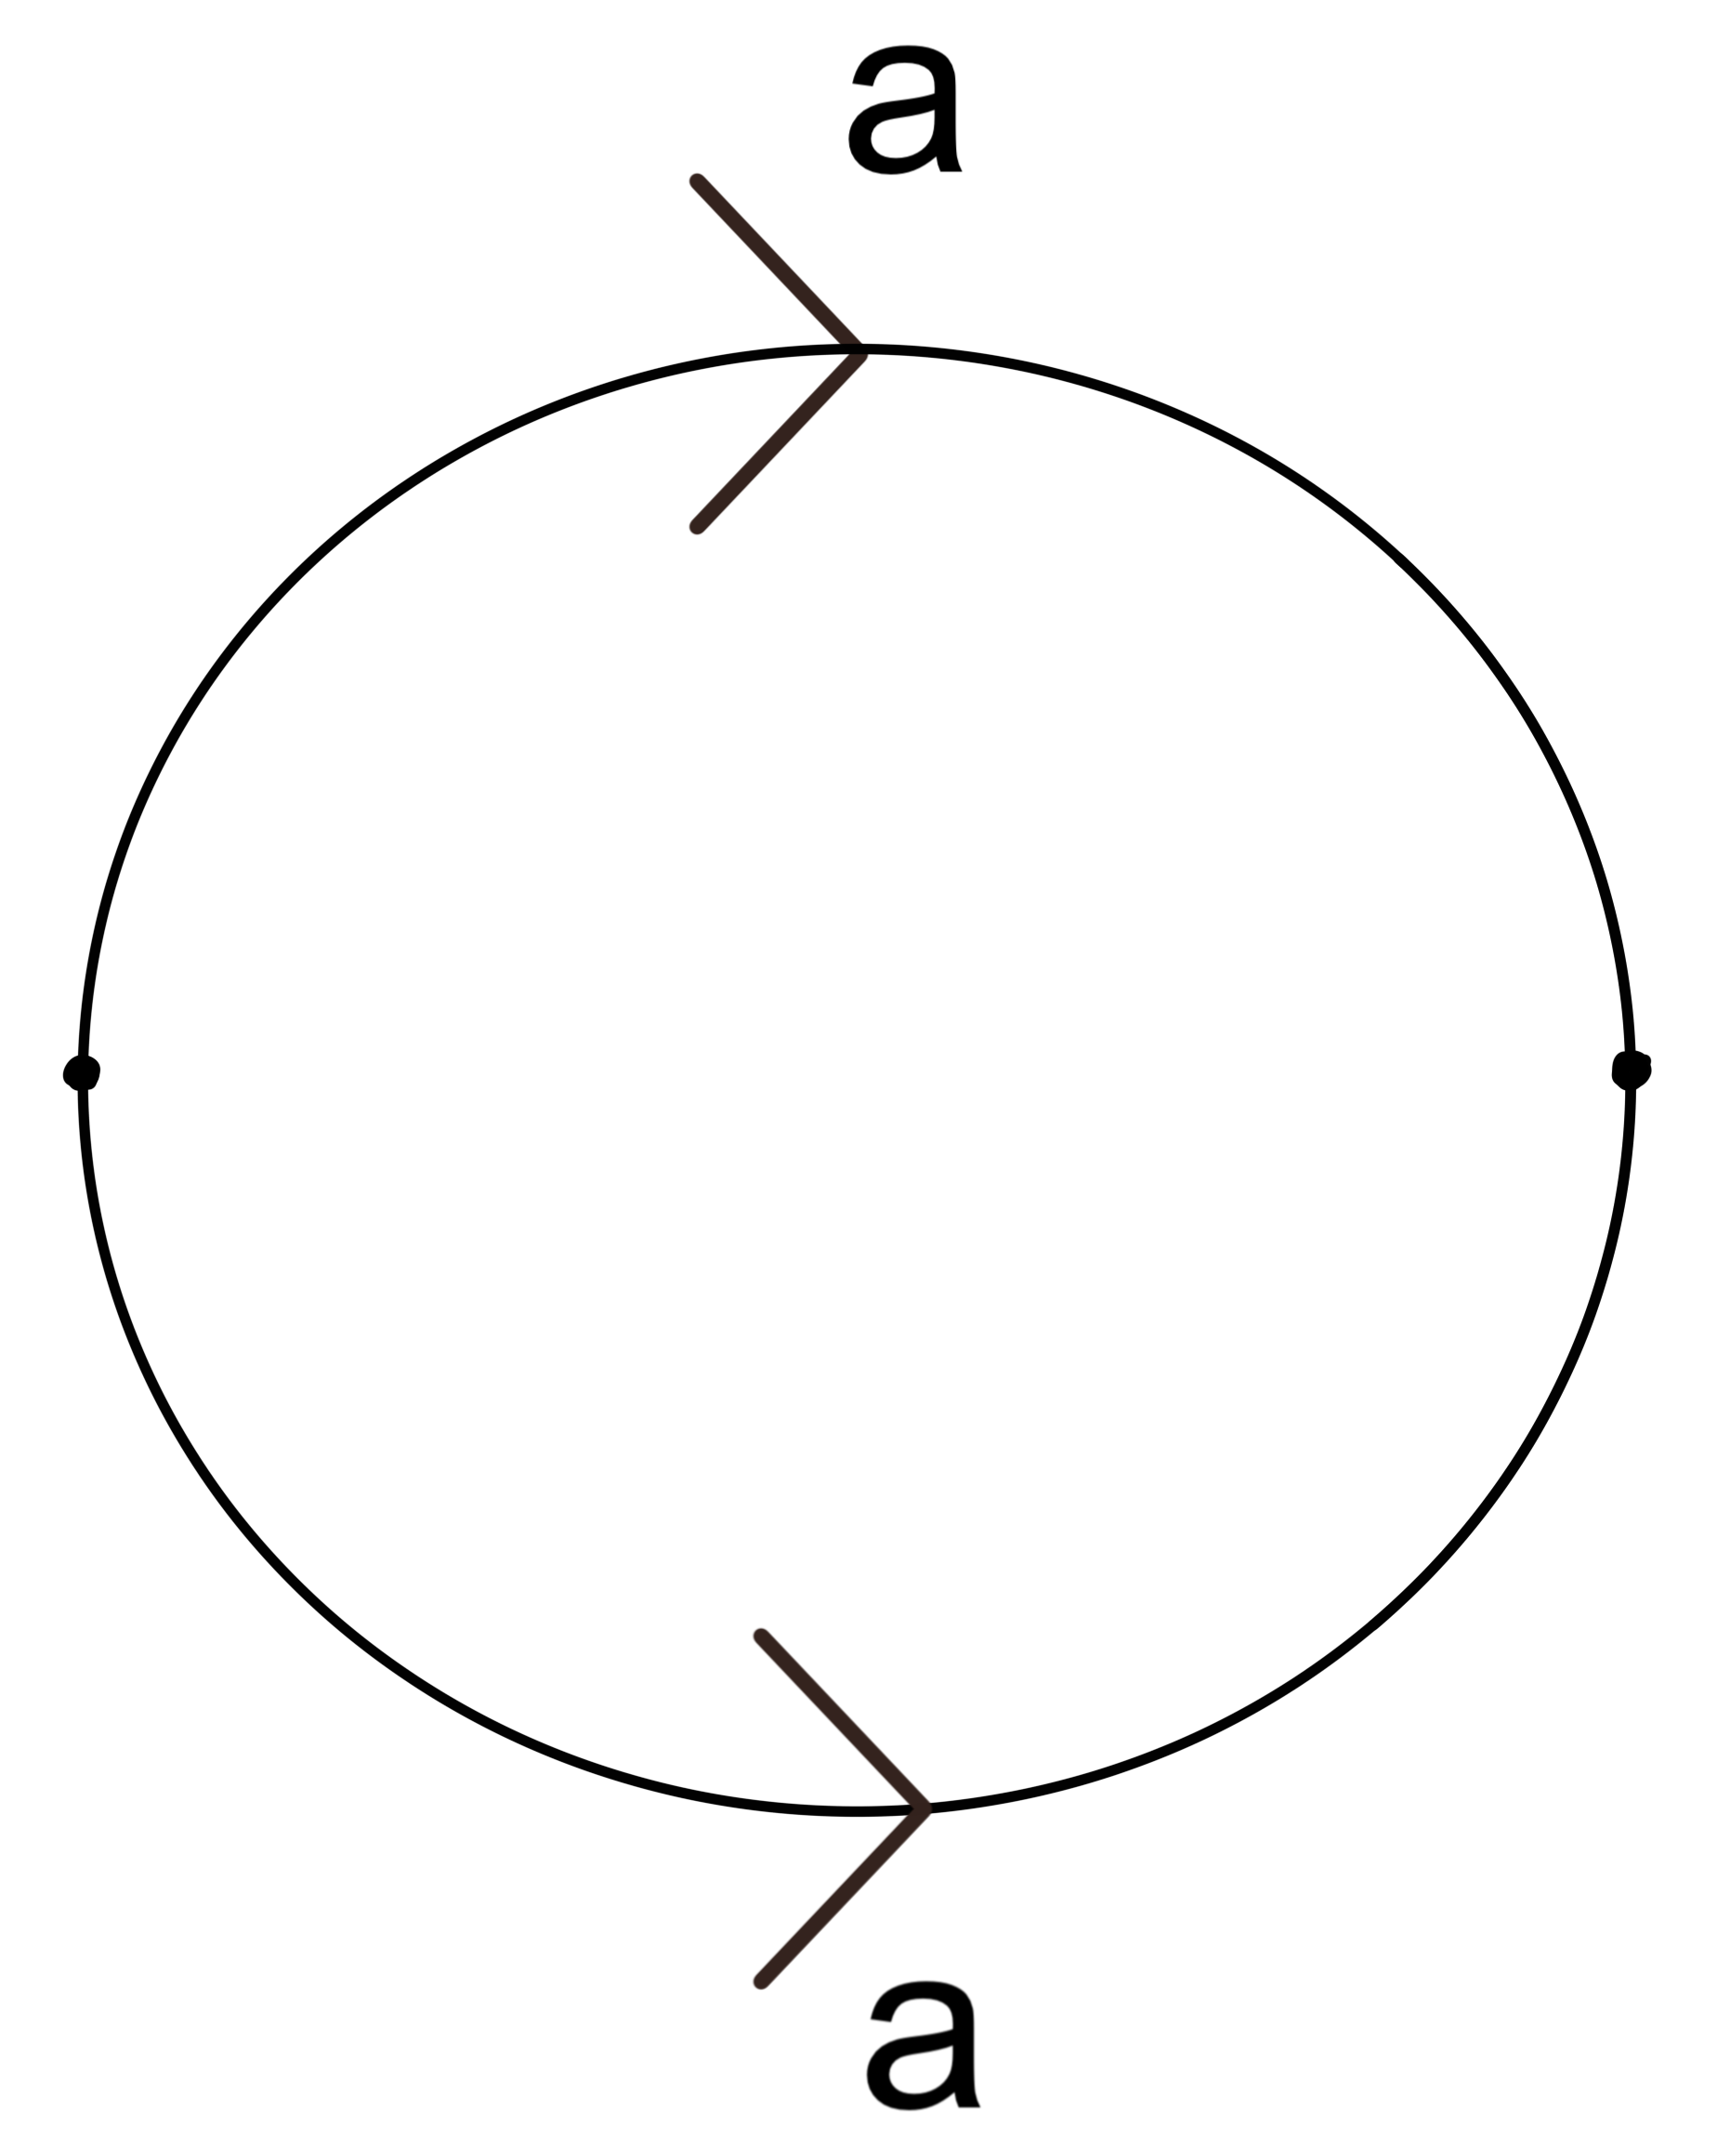
\includegraphics[width=0.15\linewidth]{imagenes/esfera_plana.png}
	\caption{Esfera como espacio cociente}
	\label{fig:esfera expresion canonica}
\end{figure} 


\subsection*{El toro}
Si se toma el cuadrado cerrado $ X = \{ (x,y) \in R^2: -1\leq x\leq 1,\quad -1\leq y \leq 1  \} $ con la topología de subespacio, el \textbf{toro}  se construye de identificar los puntos de  $ X $ según  \ref{toroid} y dotar al conjunto resultante de la topología cociente.
\begin{align}\label{toroid}
	(x,-1)\equiv(x,1) \quad x\in [-1,1]  \\
	(-1,y)\equiv(1,y) \quad y\in [-1,1] \nonumber
\end{align}
En la figura \ref{fig:toro expresion canonica} se representa gráficamente el toro. Las aristas con el mismo símbolo indican aristas a identificar en el sentido fijado por las flechas.
\begin{figure}[h!]
	\centering
	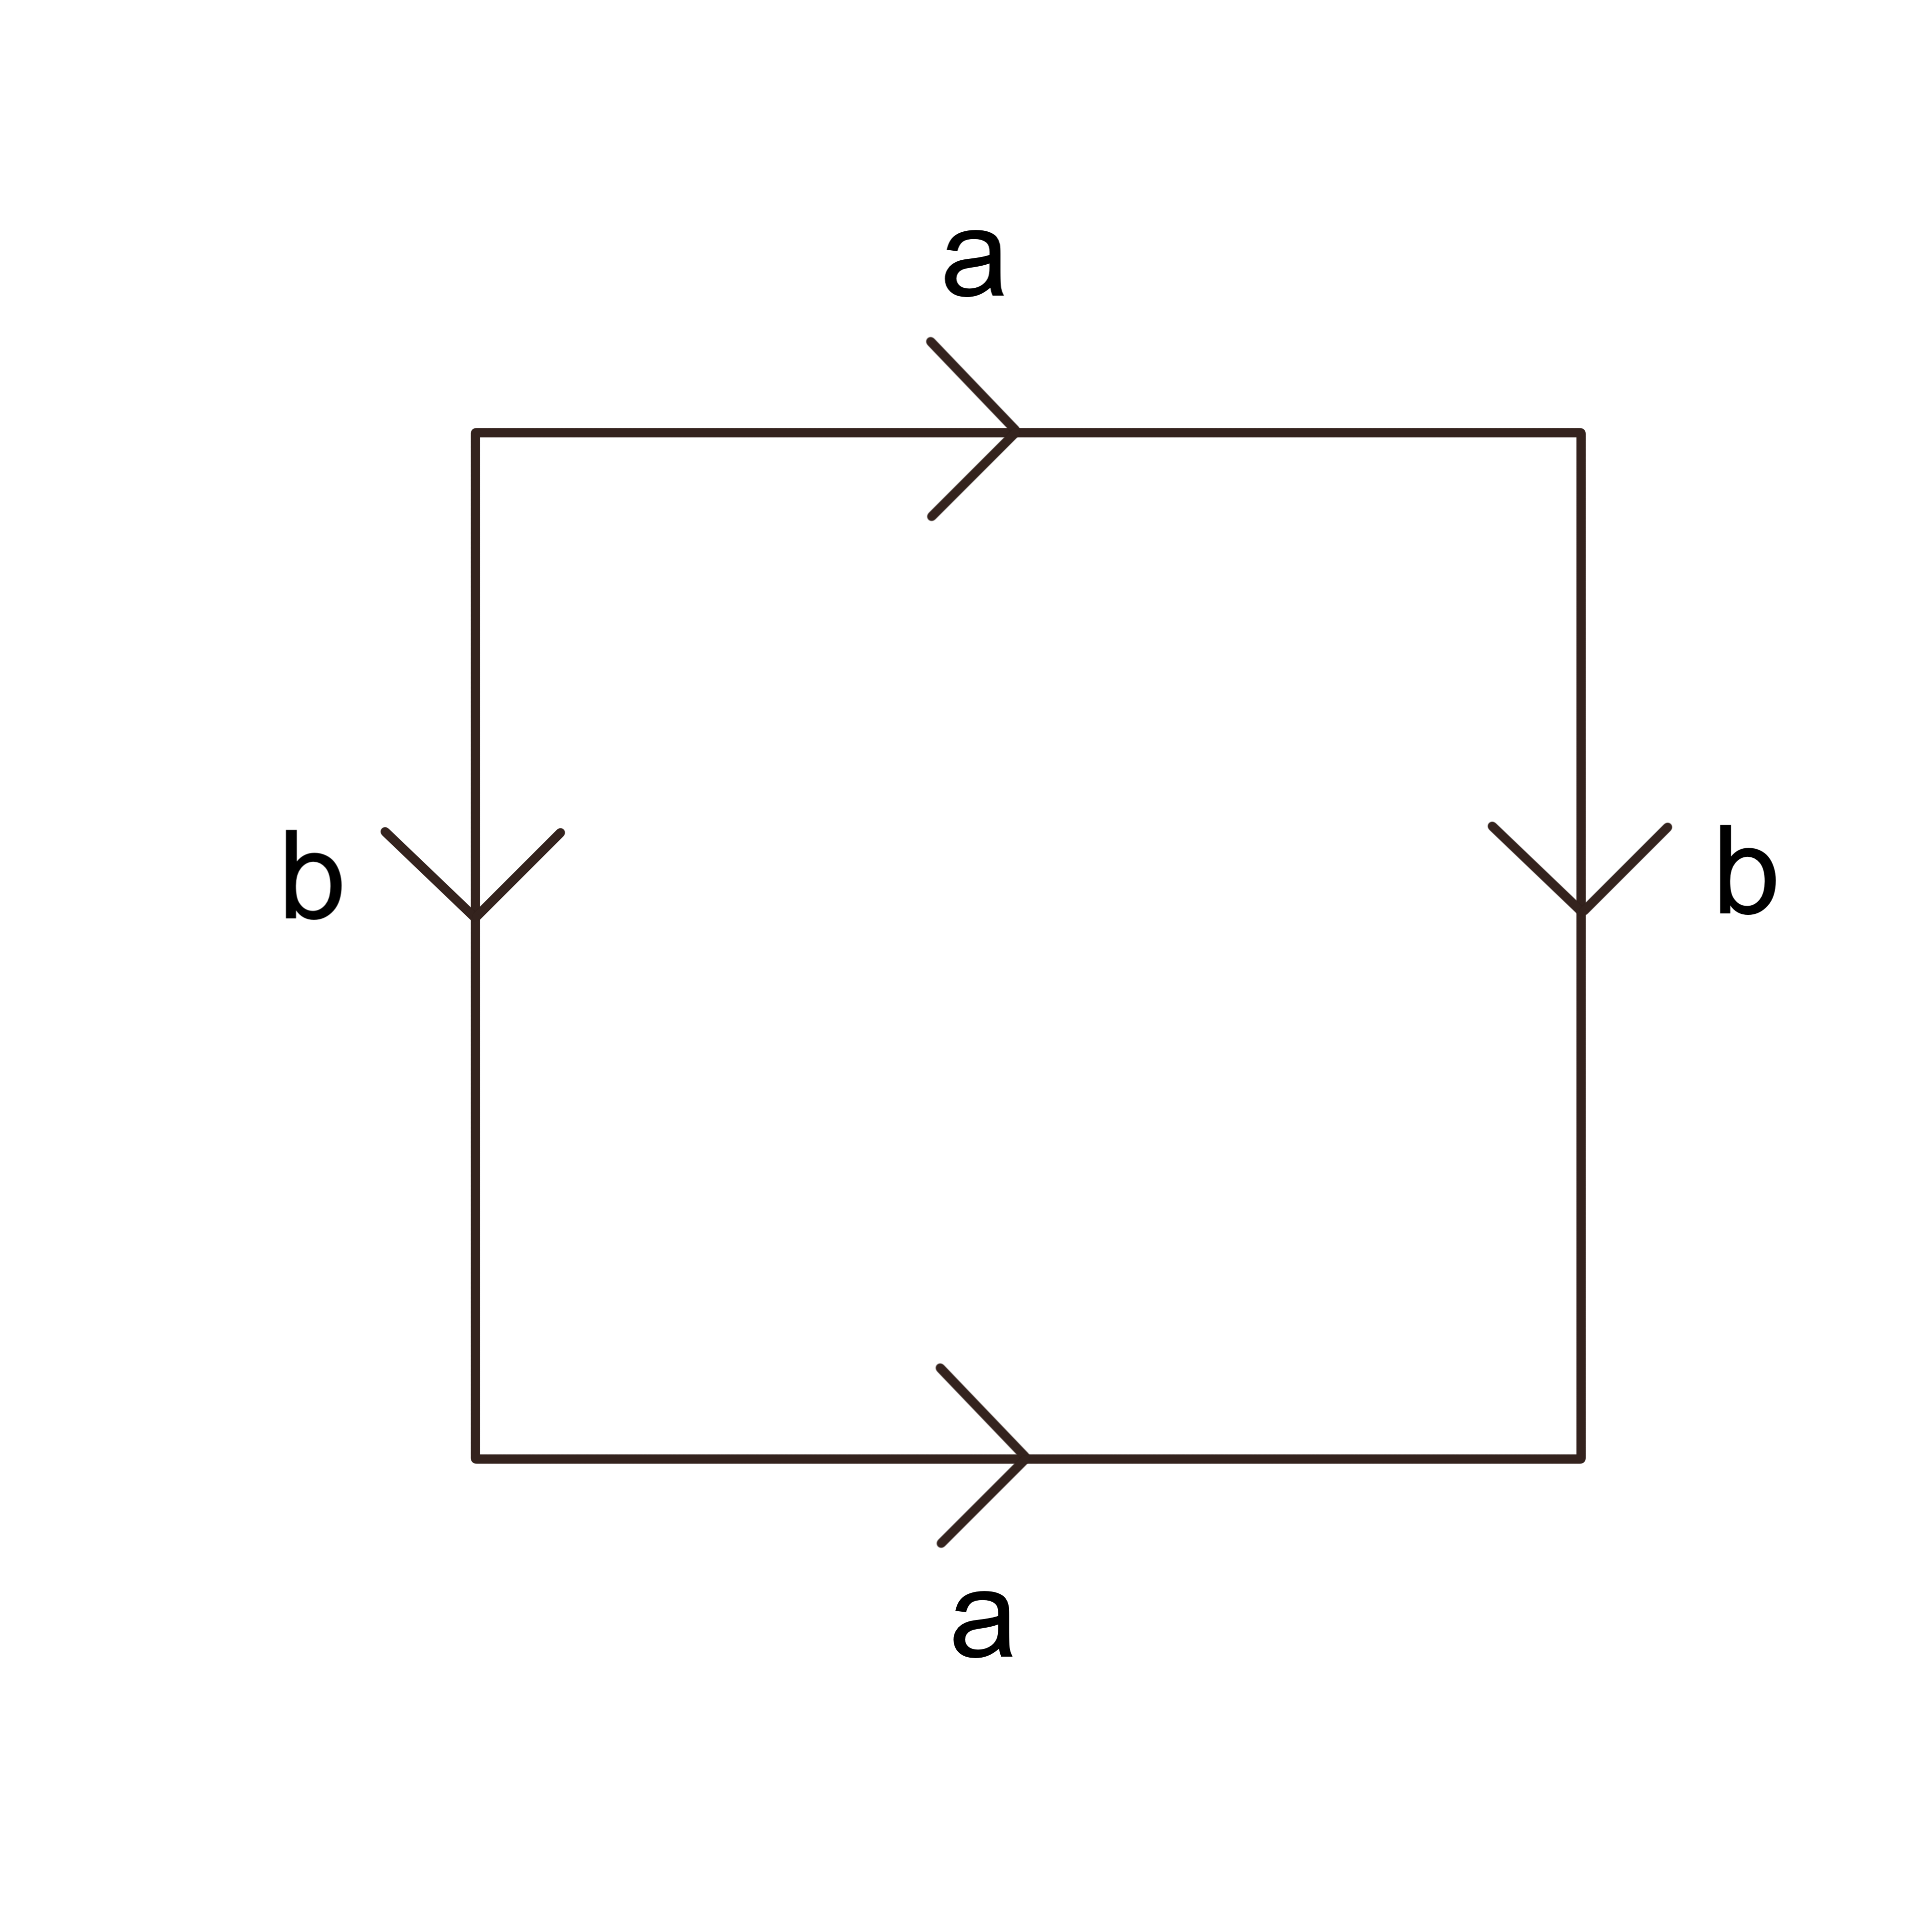
\includegraphics[width=0.2\linewidth]{imagenes/toroplano.png}
	\caption{Toro como espacio cociente}
	\label{fig:toro expresion canonica}
\end{figure} 

La definición de toro aquí expuesta es homeomorfa a la superficie de revolución en $\reales^3$ estudiada en el grado. Esta definición será conveniente más adelante en el teorema de clasificación de superficies compactas.

\subsection*{El plano proyectivo}
Por su parte, el \textbf{plano proyectivo} corresponde al disco $ D = \{x\in\mathbb{R}^2: ||x||\leq1 \} $ en el cual se identifican los puntos antipodales de la frontera. Se ilustra esta identificación en la figura \ref{fig:planoproyectivo expresión canónica}.

\begin{figure}[h!]
	\centering
	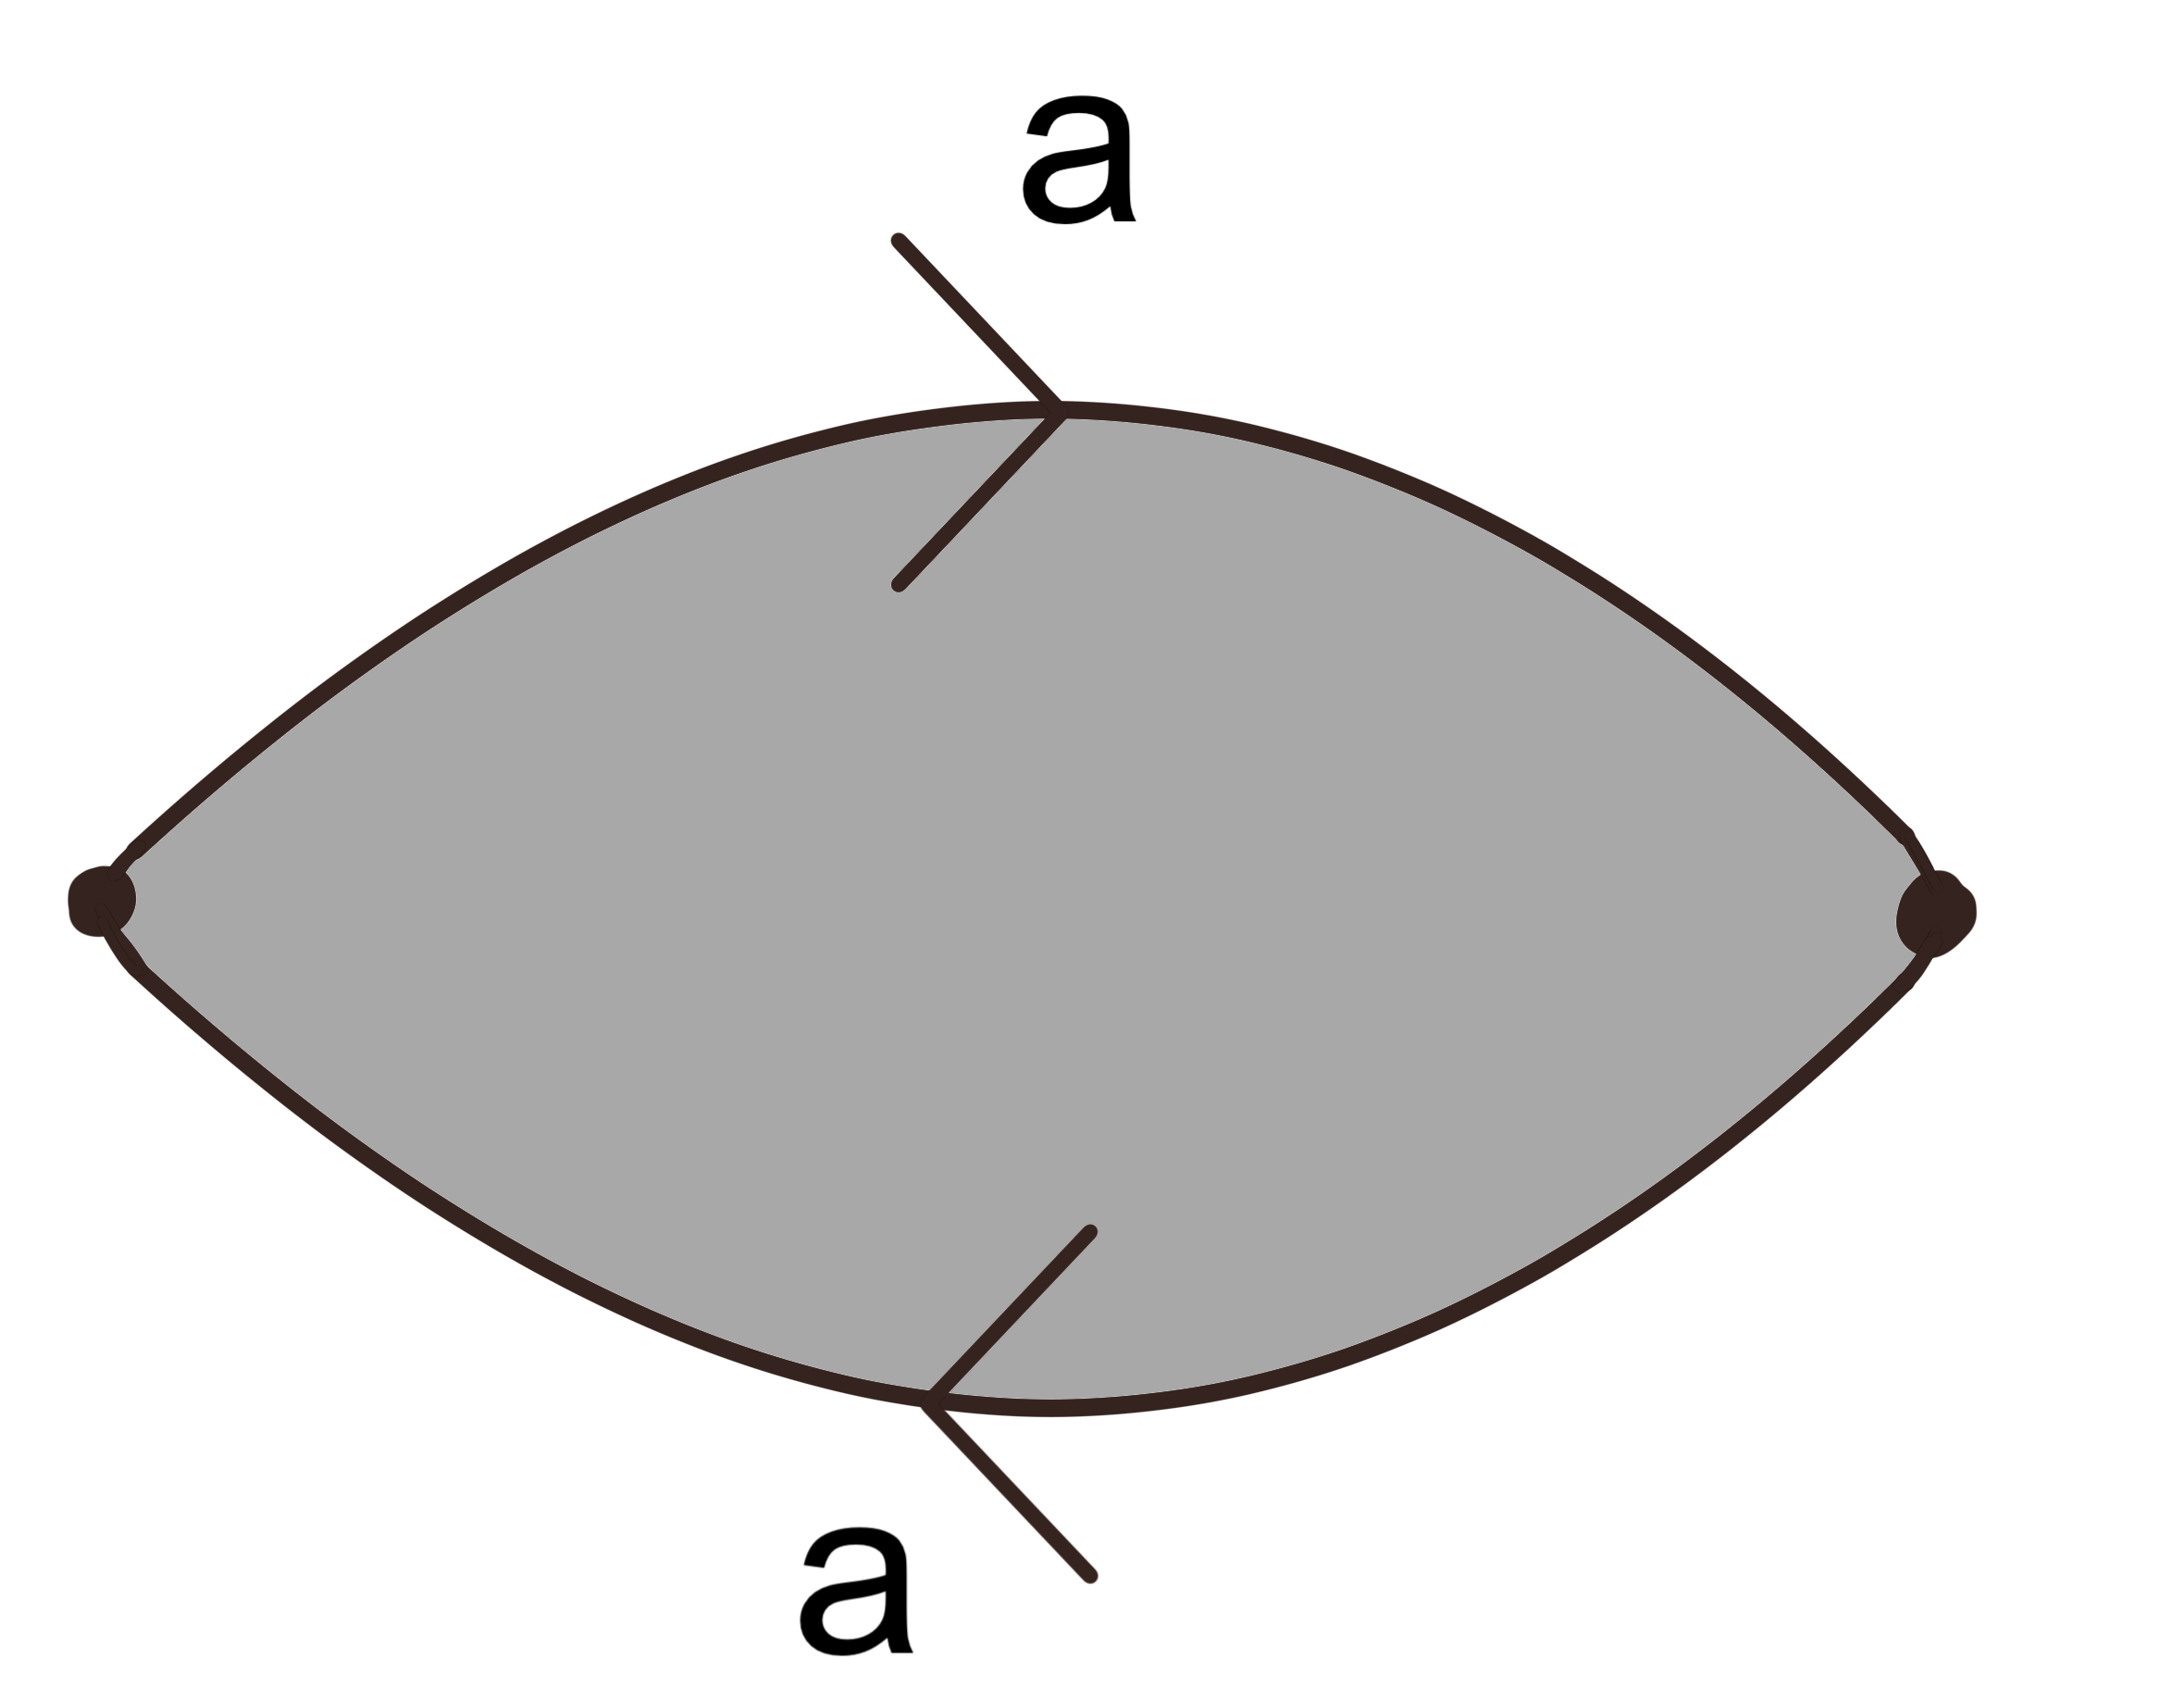
\includegraphics[width=0.3\linewidth]{imagenes/planop_plano.png}
	\caption{Plano proyectivo como espacio cociente}
	\label{fig:planoproyectivo expresión canónica}
\end{figure} 

De los tres ejemplos de superficies compactas dadas hasta ahora, este es el único de una superficie no orientable. 

Después de haber visto los ejemplos, es razonable cuestionarse si los espacios cocientes que tratamos son realmente conjuntos compactos. El siguiente lema nos demuestra que, en efecto, las superficies obtenidas son compactas.

\begin{lema}\label{lema:compacidadDePoligonos}
Sea $X$ un espacio topológico e $Y$  un espacio cociente que resulta de identificar puntos en $X$. Entonces:
\begin{align*}
	\text{$X$ compacto}\Rightarrow\text{$Y$ compacto}
\end{align*}
\end{lema}

\begin{proof}
Sea $f:X\longrightarrow Y$ la función cociente que asocia a cada punto su clase de equivalencia; $f$ es sobreyectiva y, por ser cociente, es continua.\\
Siendo $X$ compacto tenemos entonces que $f(X)=Y$ también lo es.
\end{proof}

En nuestros ejemplos todas las superficies vienen de identificar puntos en conjuntos compactos. Se sigue entonces del lema que las superficies son a su vez compactas.


\subsection{Expresión canónica}
\label{subsec:expcanonica}

Las figuras \ref{fig:esfera expresion canonica}, \ref{fig:toro expresion canonica} e \ref{fig:planoproyectivo expresión canónica}, de cada ejemplo respectivamente, sugieren una forma visual de definir superficies compactas: formamos un polígono con un número par de lados e identificamos sus aristas a pares. 

Más aún, se puede definir una notación con la que referirnos a estos polígonos: \\
Partiendo de cualquier vértice recorremos la figura en el sentido de las agujas del reloj, se anotan los símbolos según se recorre la respectiva arista y se agrega el exponente 1 o -1, según si la flecha va en el mismo sentido del recorrido o en sentido contrario.

Con esta notación: nos referimos  a la esfera (figura \ref{fig:esfera expresion canonica}) como $ aa^{-1} $; al toro (figura \ref{fig:toro expresion canonica})  como $ aba^{-1}b^{-1} $; y al plano proyectivo (figura \ref{fig:planoproyectivo expresión canónica}) como $ aa $. Llamaremos \textbf{expresión canónica} a estas formas de referirnos a la esfera, al toro y al plano proyectivo, respectivamente.

La notación sugerida facilita enormemente la definición de nuevas superficies. Utilicemos esta herramienta para introducir un último ejemplo de superficie compacta:


\subsection*{Botella de Klein}
La \textbf{botella de Klein} es la superficie que corresponde con la expresión $ aba^{-1}b $.
\begin{figure}[h!]
	\centering
	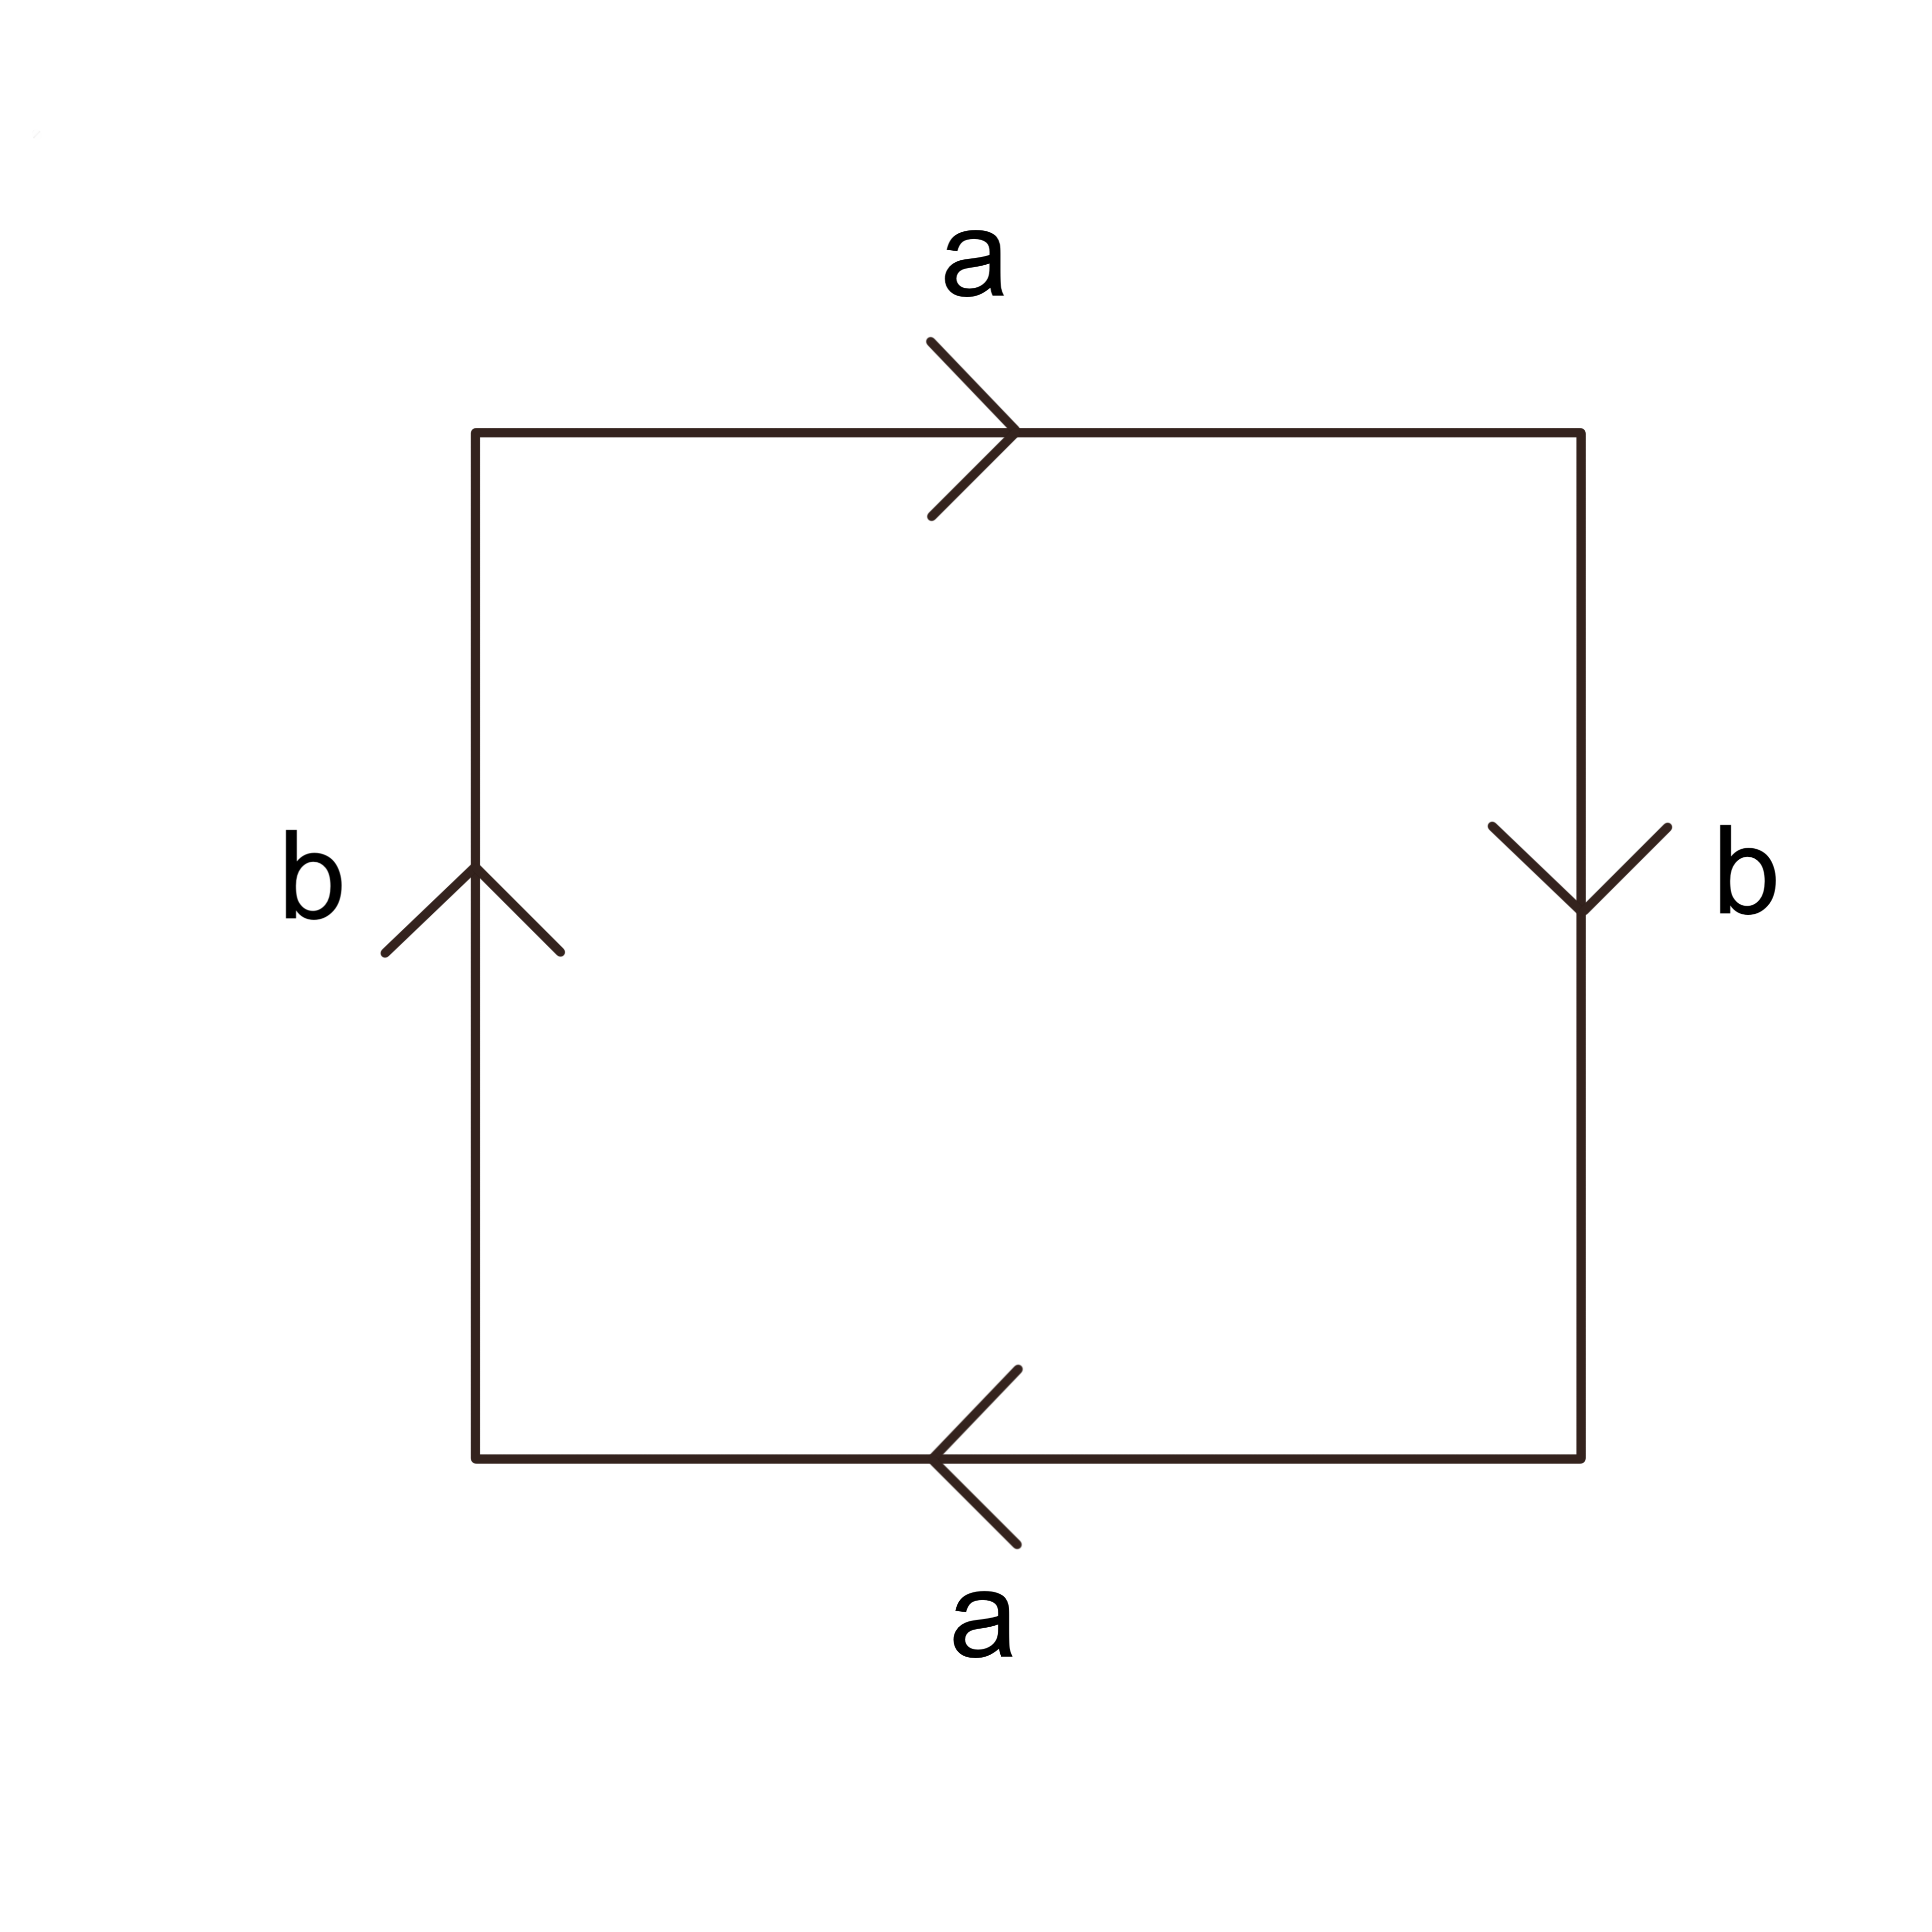
\includegraphics[width=0.2\linewidth]{imagenes/klein.png}
	\caption{Botella de Klein}
	\label{fig:botelladeklein expresion canónica}
\end{figure} 

La botella de Klein compone un ejemplo de superficie no orientable que, además, no es representable en $\reales^3$ como una superficie regular.

\section{Suma conexa}

La suma conexa es un operador entre superficies. La idea será ir \textquoteleft sumando \textquoteright superficies compactas para generar nuevas. De hecho, si se me permite el \textit{spoiler}, utilizaremos este operador en toros y planos proyectivos para construir superficies homeomorfas a \textbf{cualquier} otra superficie compacta.\\
Procedamos a definir matemáticamente el operador:

\begin{defin}\label{defin:sumaconexa}
Dadas dos superfices $S_1$ y $S_2$, se define la \textbf{suma conexa} de ambas ($S_1\#S_2$) como la superficie generada al recortar un disco de cada superficie y pegarlas a través del borde de los discos retirados. Más formalmente:
\begin{enumerate}
\item  Para cada $S_i$, tomamos un subconjunto $D_i\subset S_i$ homeomorfo al disco cerrado $E^2=\{x\in\mathbb{R}^2: ||x||\leq 1\}$. Llamamos $S'_i$ al complementario del interior de $D_i$.

\item Tomamos un homeomorfismo $\psi:D_1\longrightarrow D_2$

\item Definimos entonces $S_1\#S_2$ como $S'_1\cup S'_2$ dotado de la topología cociente que resulta de la identificación:
\[ x \equiv  \psi(x), \quad \forall x \in D_1 \] 
\end{enumerate}
Habría que comprobar que la suma conexa está bien definida y resulta en una nueva superficie. Este aspecto lo abordamos en lema \ref{lema:sumaconexa}.
\end{defin}


\subsection*{Ejemplos}
Utilizando la notación introducida hasta el momento presentamos algunos ejemplos de sumas conexas:

\noindent \textbf{Suma conexa de toros}
\\
Sean $ T_1 $ y $ T_2 $ dos toros disjuntos, estudiemos $ S=T_1\, \# \, T_2 $. Nos ayudamos de la figura \ref{fig:suma conexa de toros planos} para ilustrar el proceso:\\
Primero, retiramos de cada toro el disco con frontera $c_i$, como vemos en la primera imagen. Nótese que podemos expresarlo como la segunda imagen porque todos los vértices del polígono están identificados. Finalmente, identificamos los bordes $ c_1 $ y $ c_2 $, obteniendo el octágono que representa  $ S $, donde, de nuevo, todos los vértices representan el mismo punto.

\begin{figure}[h!]
	\centering
	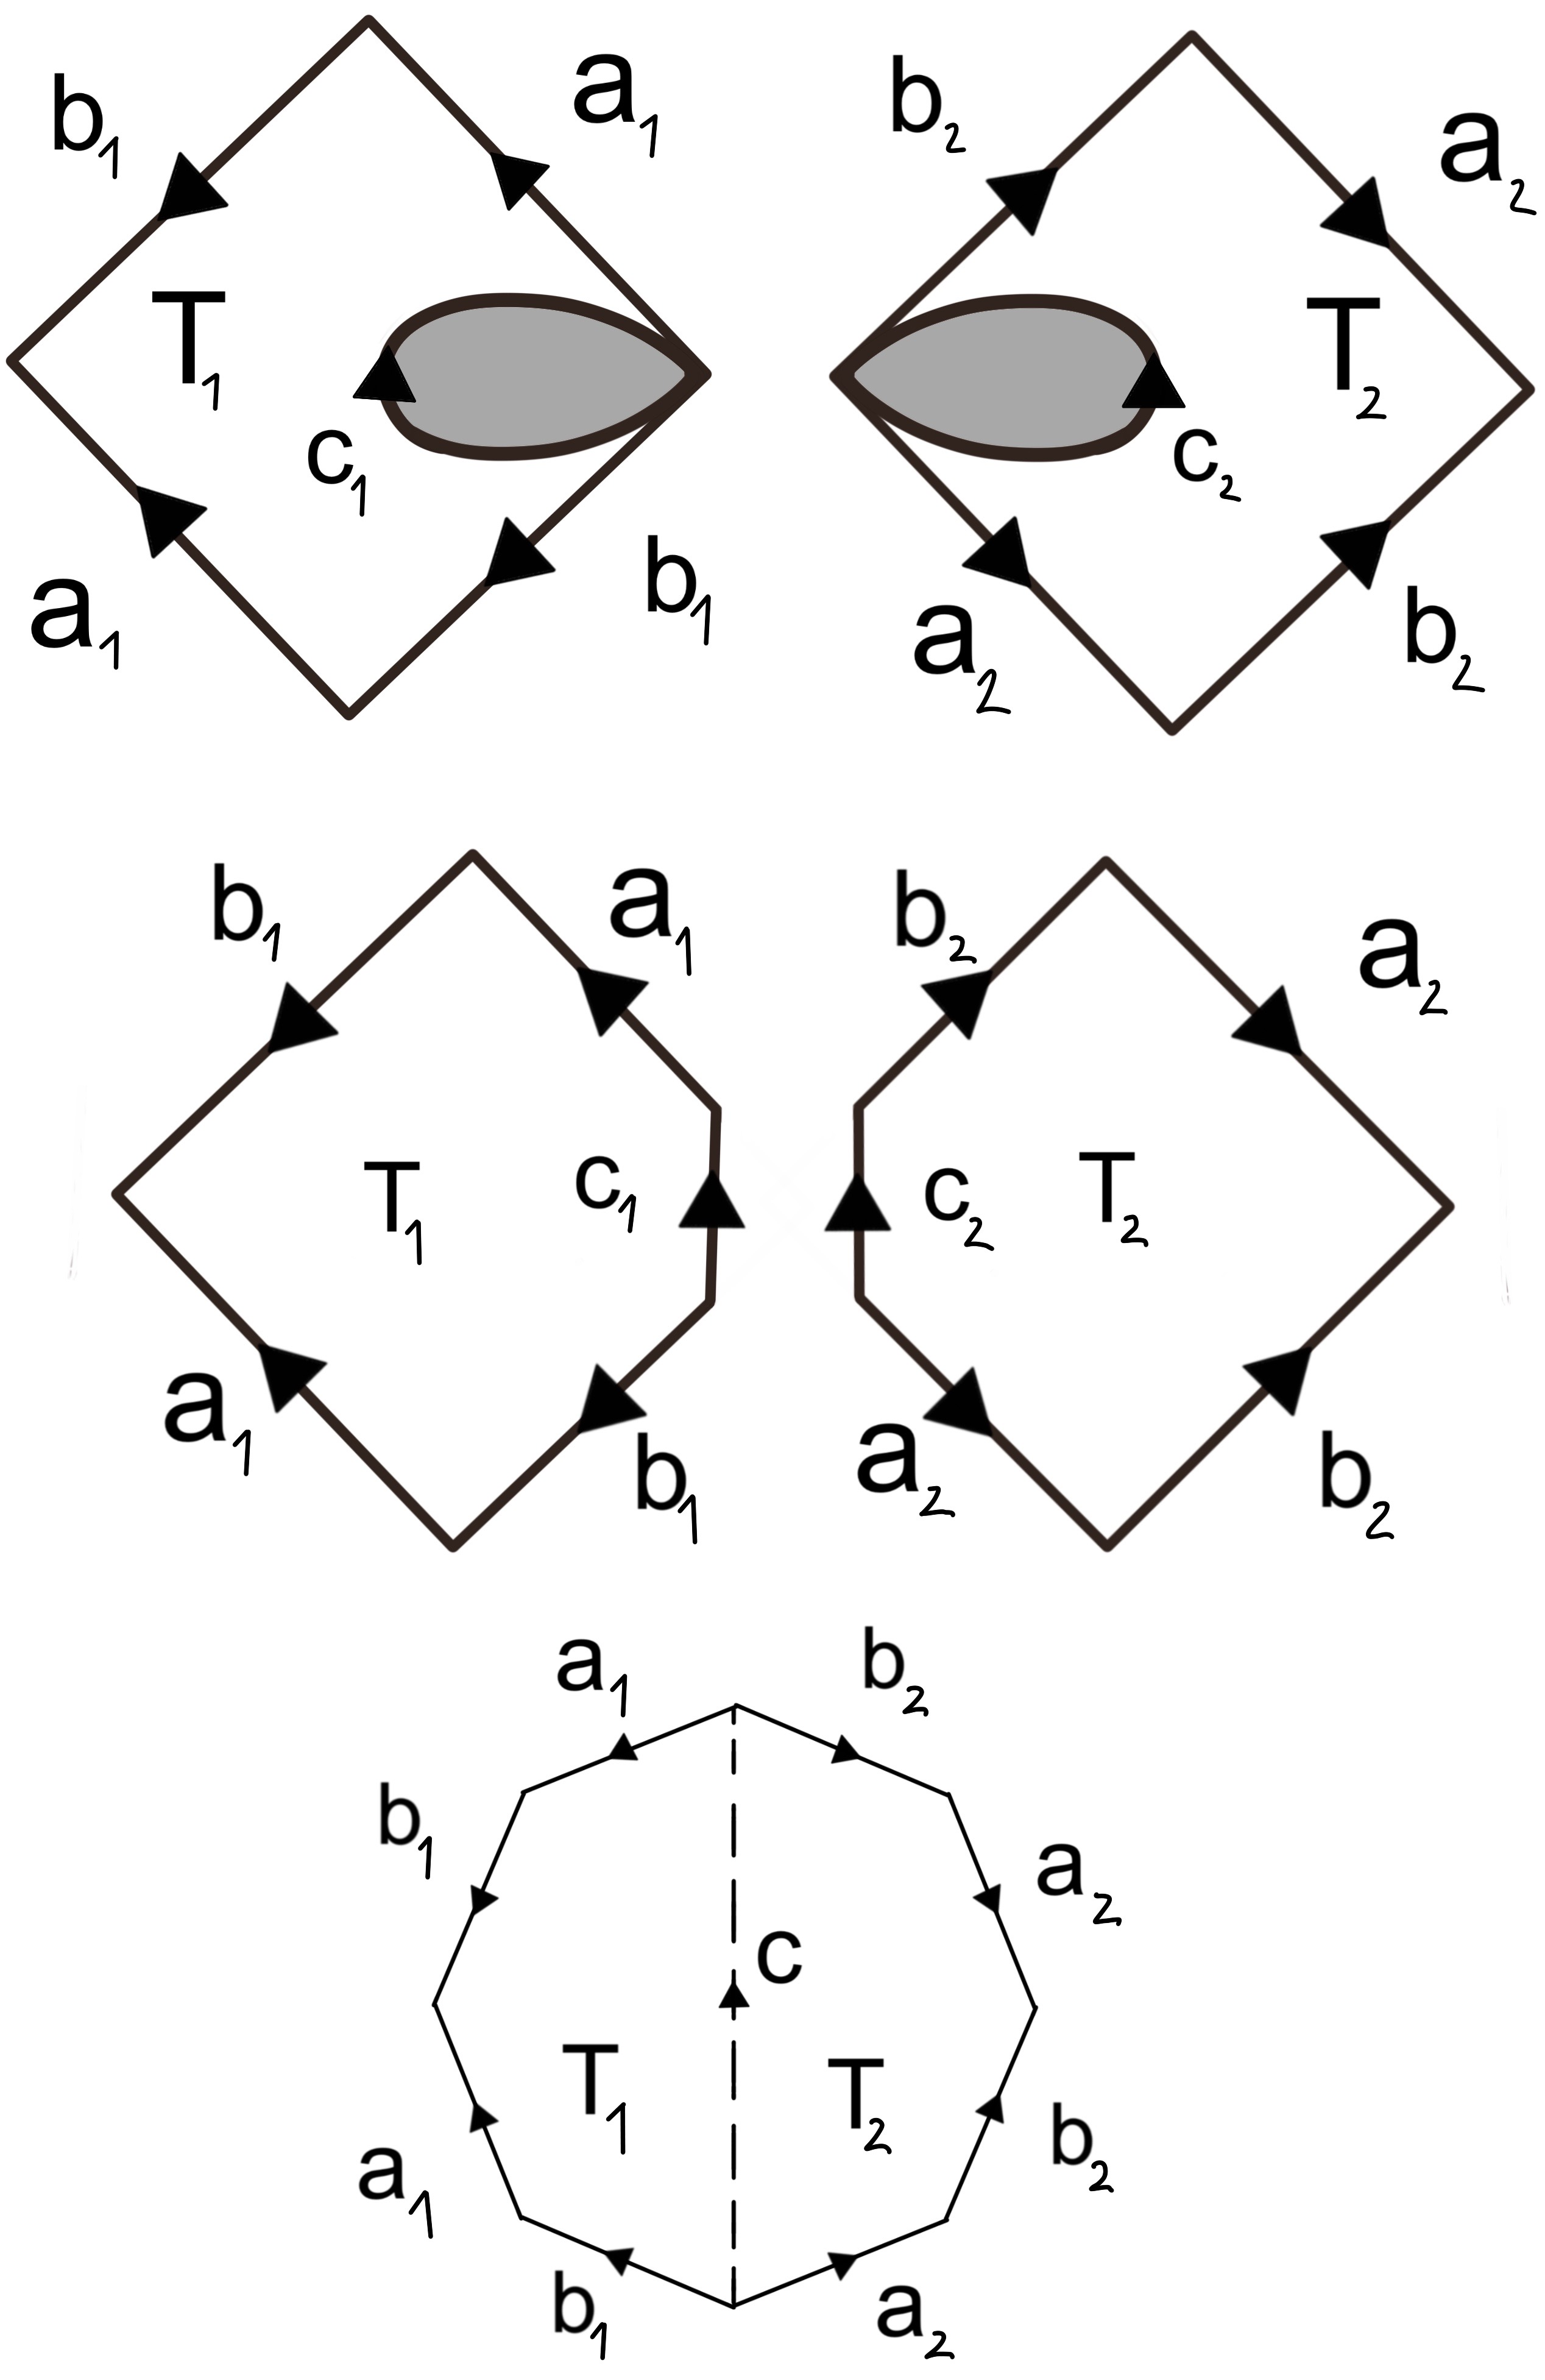
\includegraphics[width=0.4\linewidth]{imagenes/sumaconexa_toros.png}
	\caption{Suma conexa de dos toros}
	\label{fig:suma conexa de toros planos}
\end{figure} 

Utilizando la notación para expresiones canónicas, de la figura \ref{fig:suma conexa de toros planos} se deduce que  $ S $ se puede expresar como $ a_1 b_1 a_1^{-1}b_1^{-1}a_2 b_2 a_2^{-1} b_2^{-1}  $. 

\begin{figure}[h!]
	\centering
	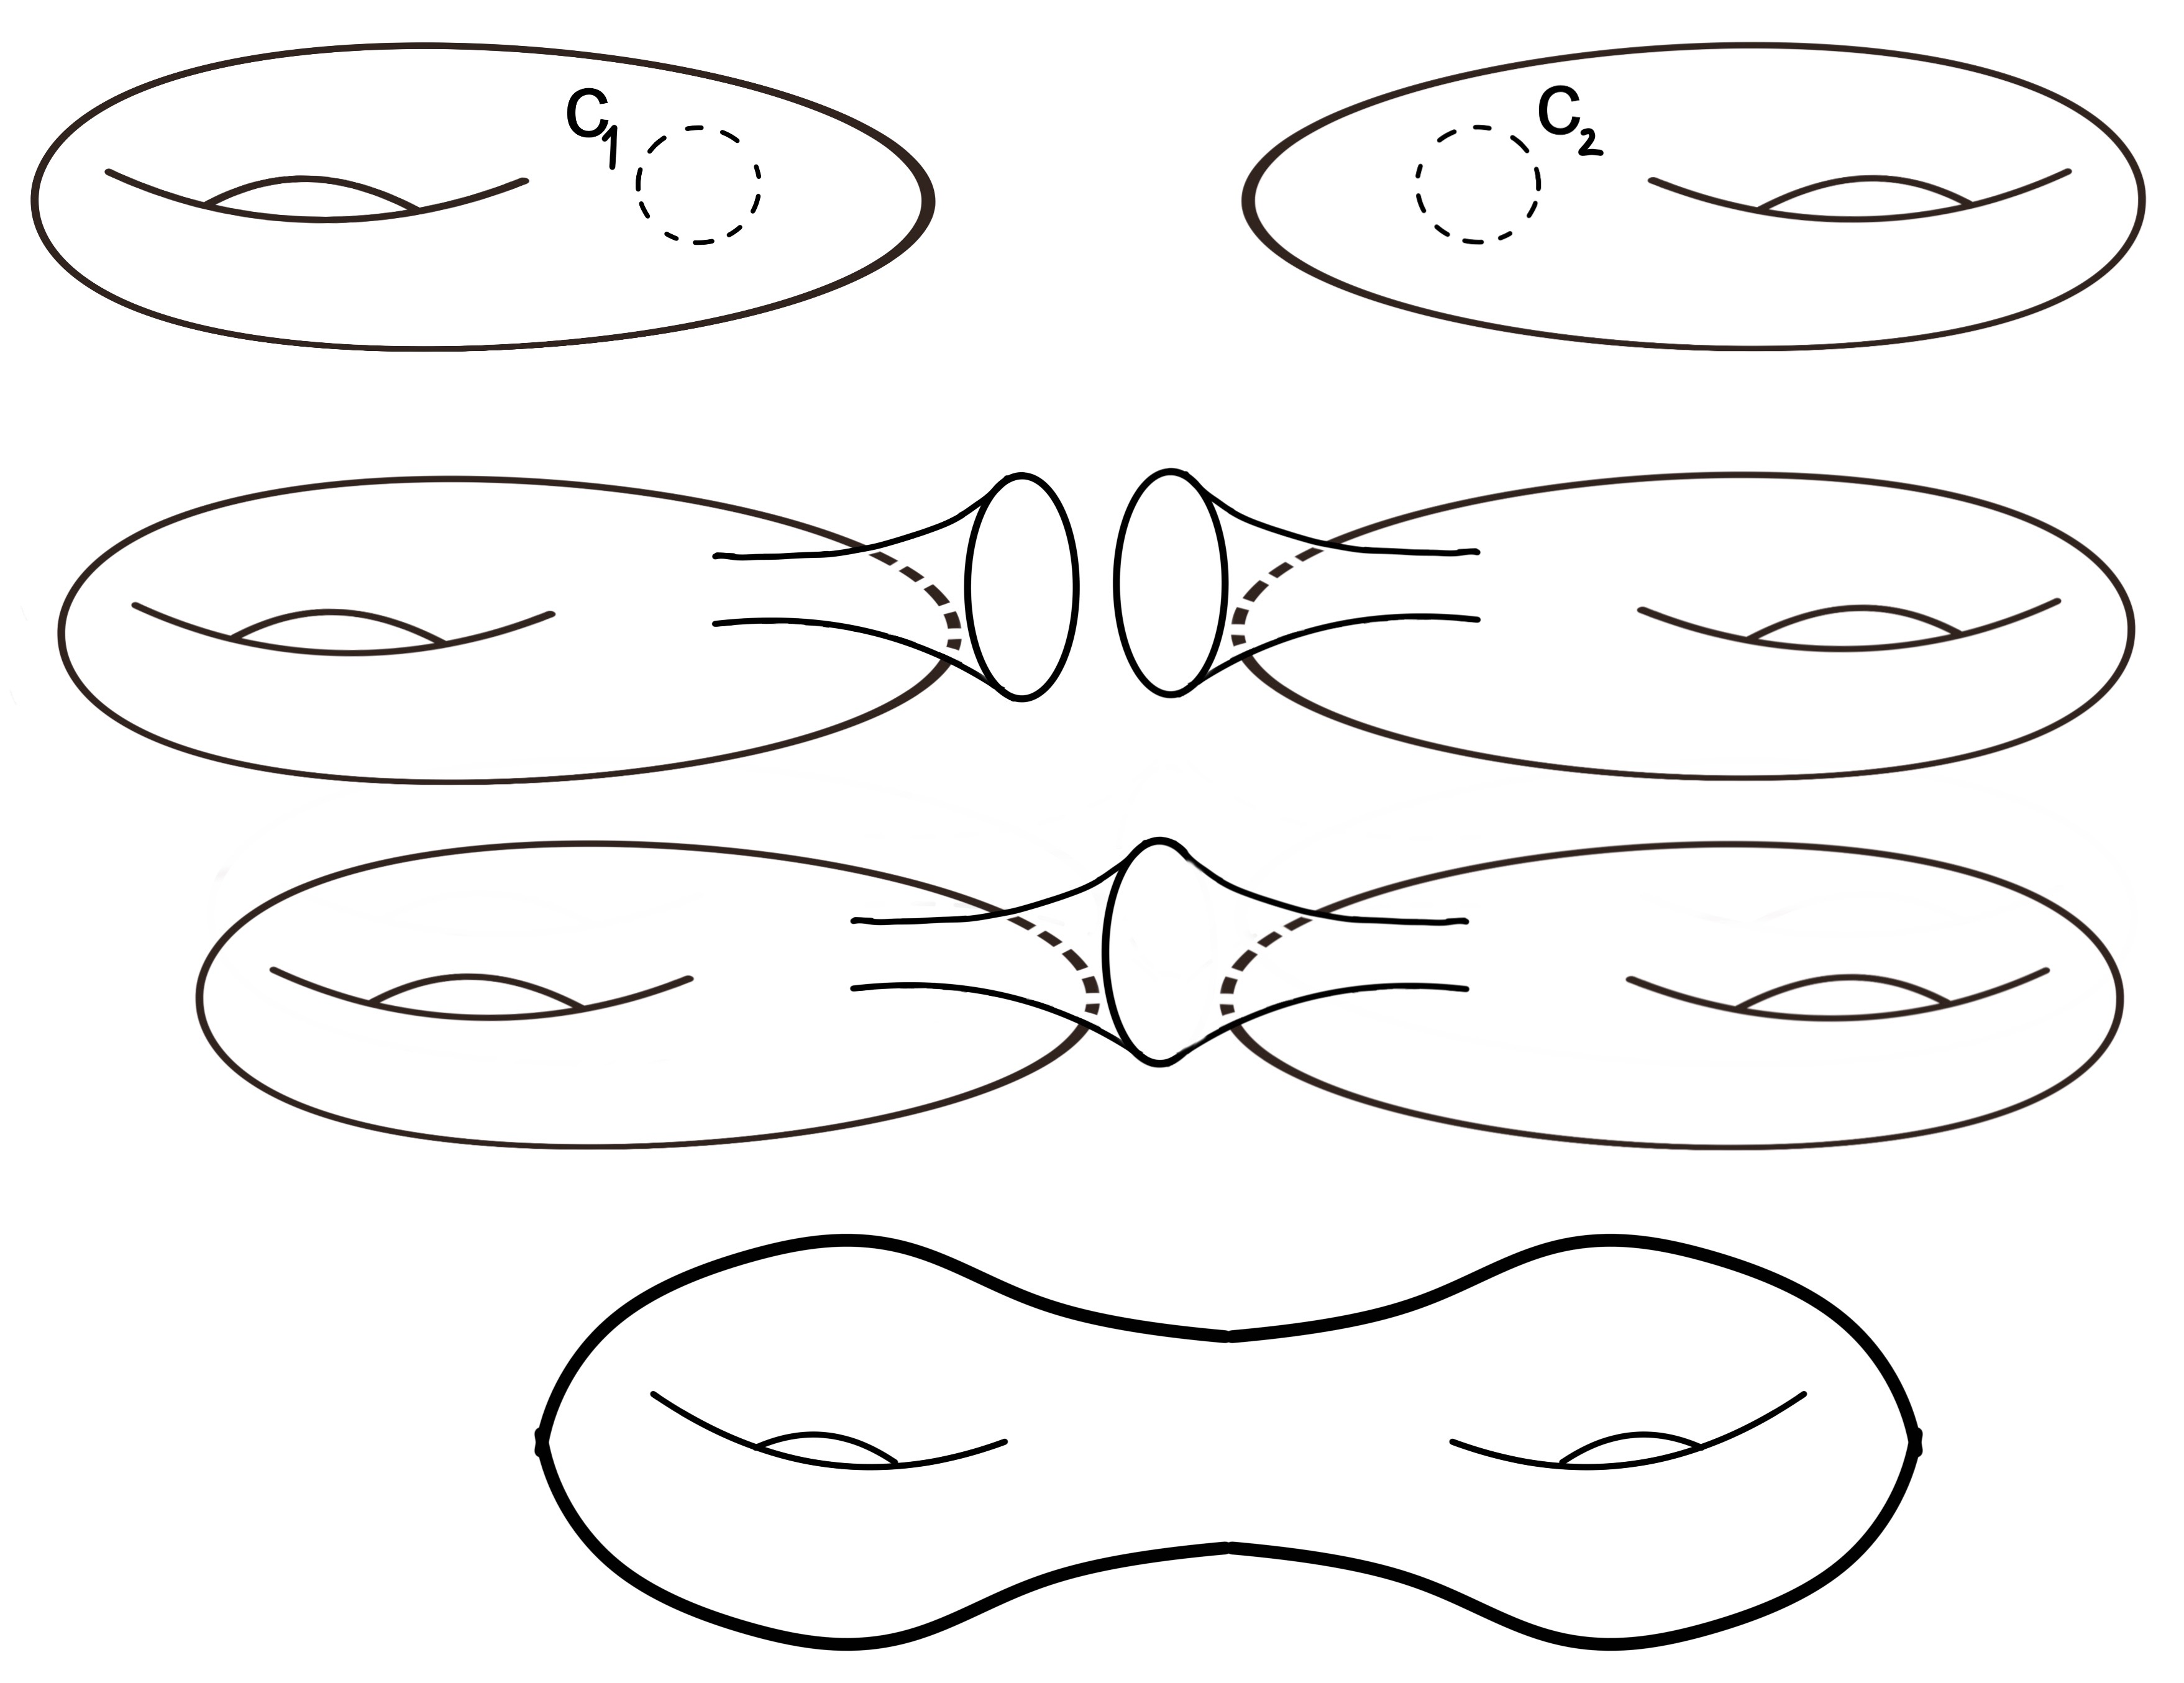
\includegraphics[width=0.4\linewidth]{imagenes/sumaconexa_toros_R3.png}
	\caption{Suma conexa de dos toros como subvariedades de $ \mathbb{R}^3 $}
	\label{fig:suma conexa de toros en R3}
\end{figure} 

\noindent \textbf{Suma conexa de planos proyectivos}
\\
Podemos seguir un mecanismo parecido al anterior para realizar la suma conexa de dos planos proyectivos. En la figura \ref{fig:suma conexa de planos p} ilustramos la misma construcción para dos planos proyectivos. La expresión canónica de la superficie resultante es $ a_1a_1a_2a_2 $.

\begin{figure}[h!]
	\centering
	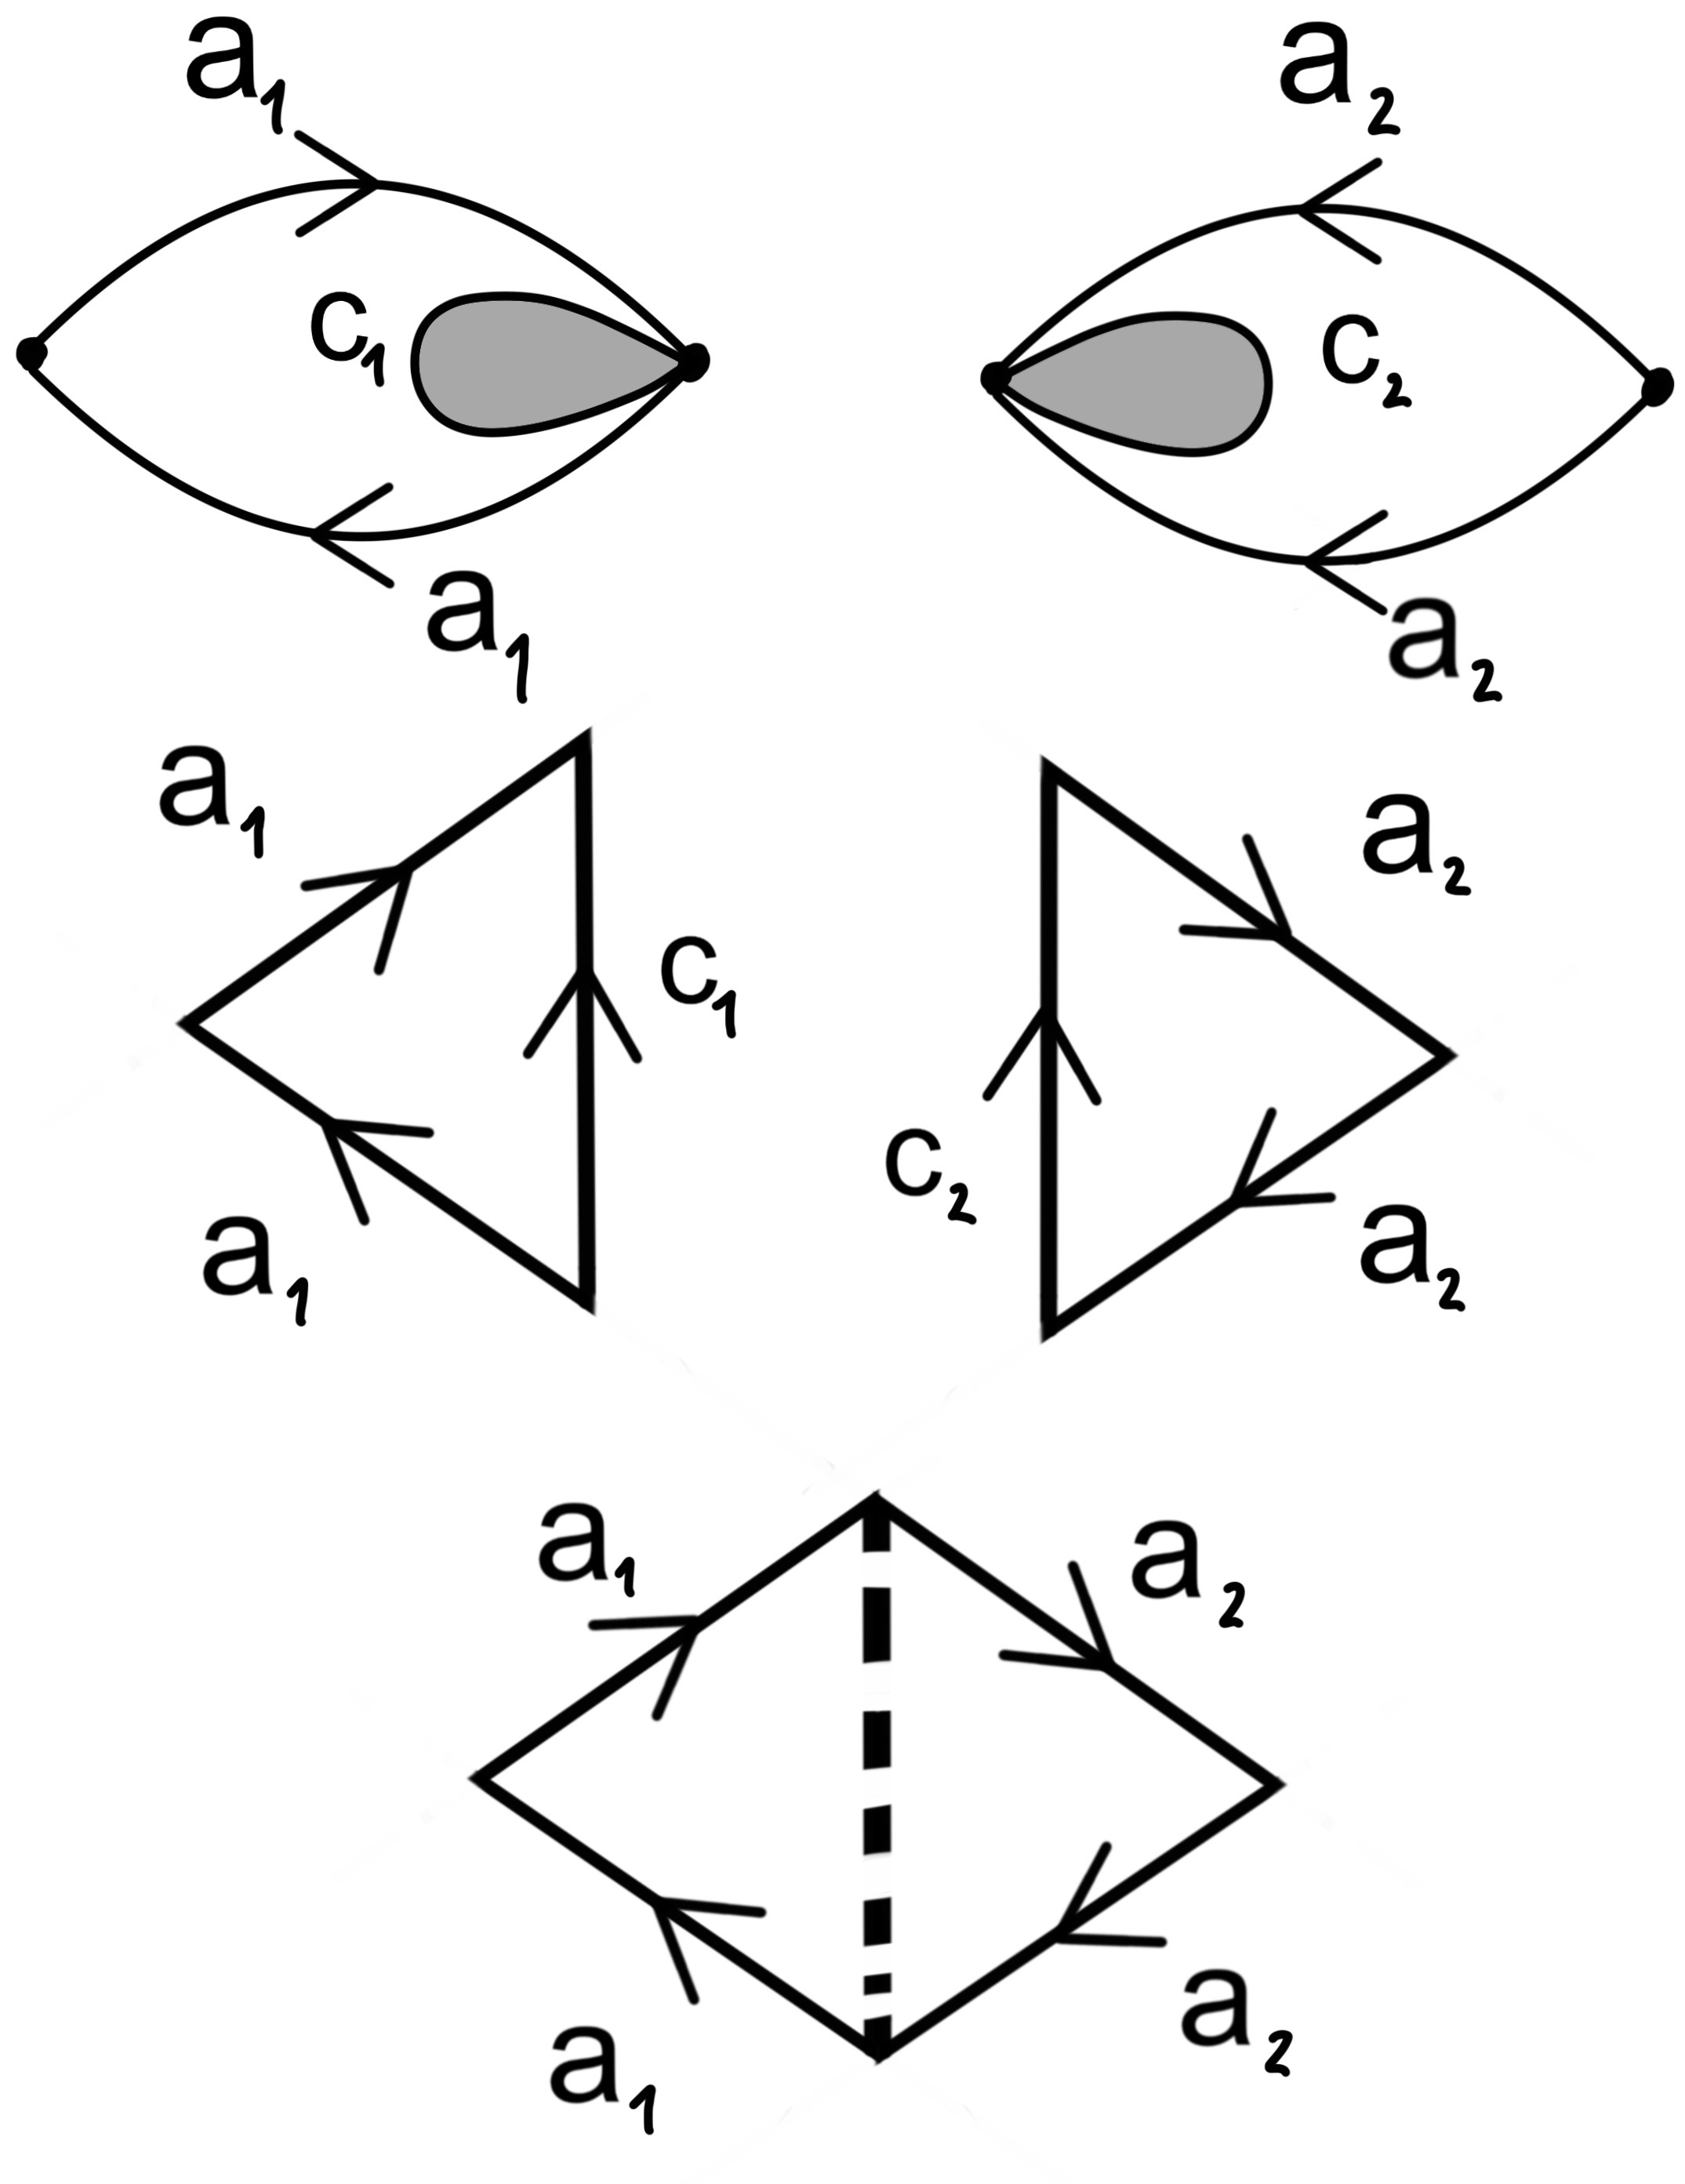
\includegraphics[width=0.3\linewidth]{imagenes/sumaconexa_planosp.png}
	\caption{Suma conexa de dos planos proyectivos}
	\label{fig:suma conexa de planos p}
\end{figure} 

\noindent \textbf{Suma conexa de esferas}
\\
En la figura \ref{fig:suma conexa de esferas} ilustramos la suma conexa de dos esferas, que es otra esfera. En general, se puede comprobar que la esfera actúa como elemento neutro de la suma conexa.

\begin{figure}[h!]
	\centering
	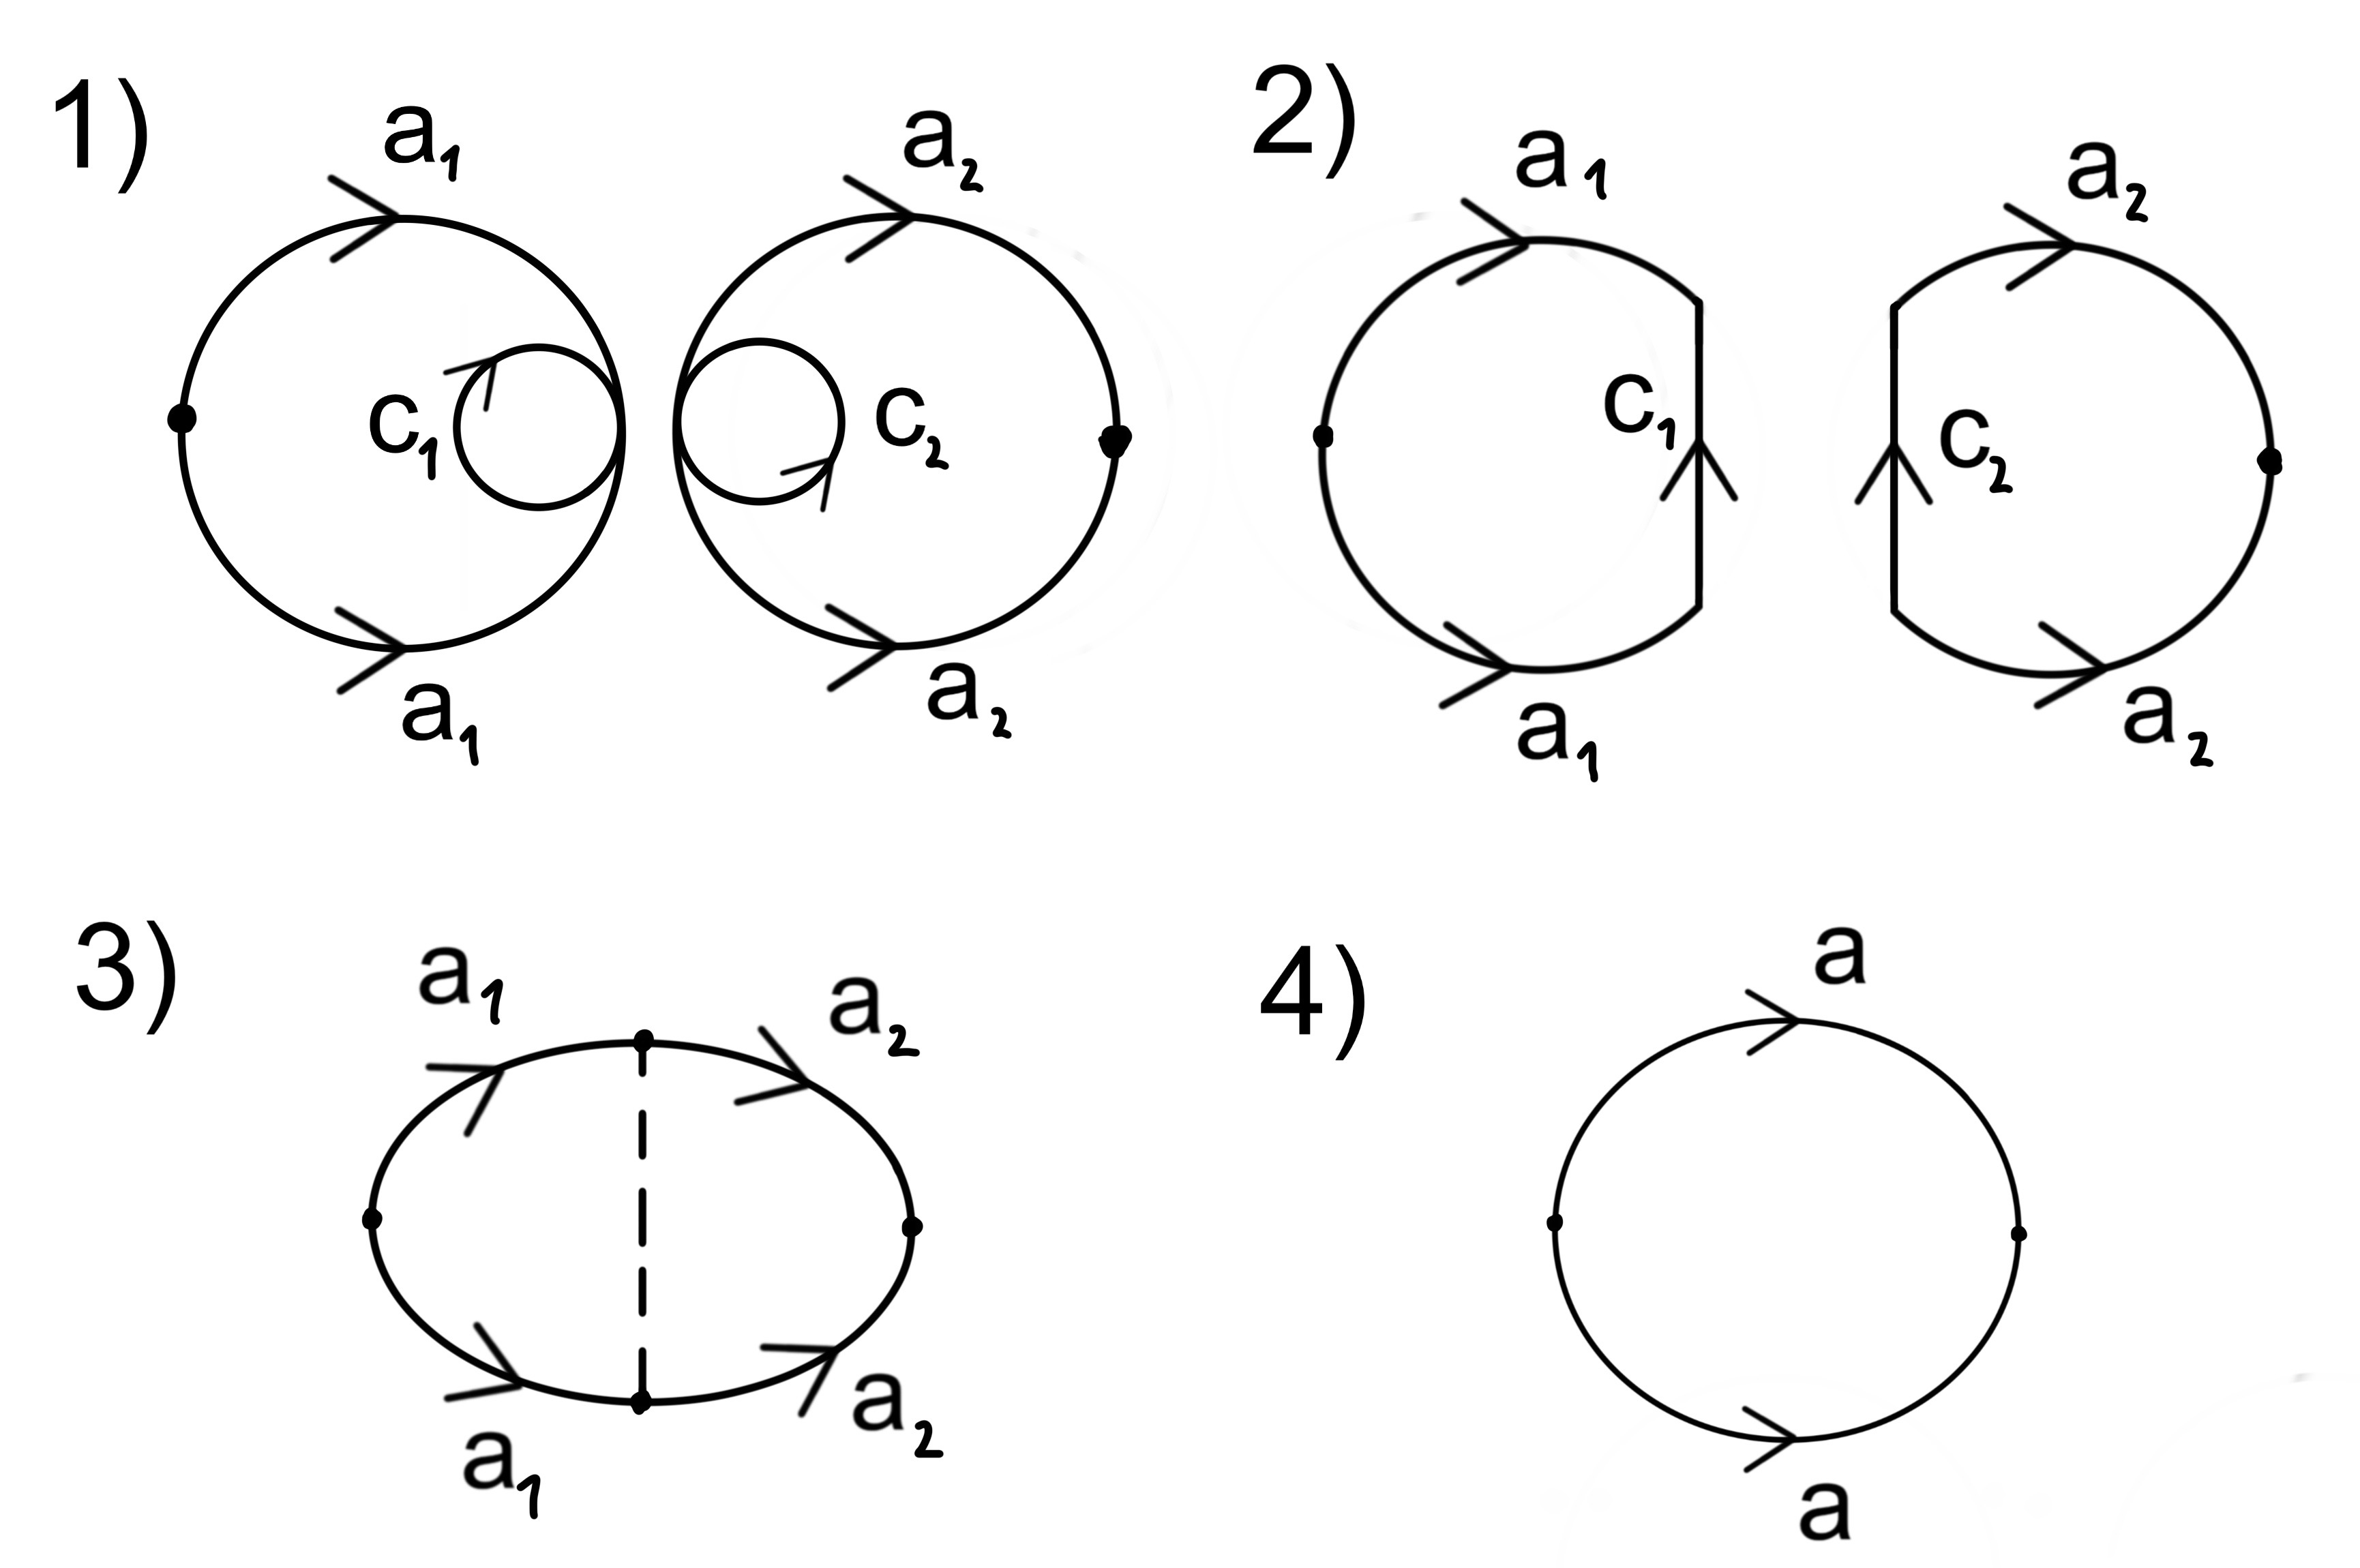
\includegraphics[width=0.5\linewidth]{imagenes/sumaconexa_esferas.png}
	\caption{Suma conexa de dos esferas}
	\label{fig:suma conexa de esferas}
\end{figure} 

Otra propiedad interesante de la suma conexa es que conserva la compacidad, i.e, si $S=S_1 \, \# \, S_2$, entonces $S$ será compacta si lo son $S_1$ y $S_2$. En los ejemplos de la suma de toros, planos proyectivos y esferas, basta con usar el lema \ref{lema:compacidadDePoligonos} para demostrarlo.

\subsection{Expresiónes canónicas de sumas conexas}
\label{subsec:expresionescanonicassumasconexas}
Los ejemplos mencionados en la sección anterior proporcionan un método para describir sumas conexas arbitrarias de esferas, toros y planos proyectivos. Basta repetir los mismos procedimientos para comprobar que:

\begin{list}{-}{}
\item La suma conexa de $ n $ esferas es igual a una esfera:
\begin{align}\label{formacanonica:esfera}
	aa^{-1} 
\end{align}

	\item La suma conexa de $ n $ toros se puede escribir como:
\begin{align}\label{formacanonica:ntoros}
	a_1b_1a_1^{-1}b_1^{-1}a_2b_2a_2^{-1}b_2^{-1}...a_nb_na_n^{-1}b_n^{-1}
\end{align}

	\item La suma conexa de $ n $ planos proyectivos se puede describir como: 
\begin{align}\label{formacanonica:nplanosp}
a_1a_1a_2a_2...a_na_n
\end{align}
\end{list}
A las expresiones \ref{formacanonica:esfera},\ref{formacanonica:ntoros} y \ref{formacanonica:nplanosp} las llamaremos \textit{expresiones canónicas} de sus respectivas sumas conexas.
 
Antes de dar el asunto por concluido, veamos un último ejemplo de suma conexa:

\begin{lema}\label{lema:SumaDosPlanospEsKlein}
La suma conexa de dos planos proyectivos es homeomorfa a una botella de Klein

\begin{proof}
En la demostración trataremos al plano proyectivo como el disco unidad identificando los puntos diametralmente opuestos.\\
Seleccionamos del plano proyectivo el subconjunto $D = \left\{(x,y): ||y||\geq\frac{1}{2}, ||x||\leq\sqrt{1-y^2} \right\}$  homeomorfo al disco cerrado. Retiramos $ D $ como se muestra en la figura \ref{fig:planop sin D}, los segmentos discontinuos representan la frontera del disco por la cual se ha de realizar la suma conexa.

\begin{figure}[h!]
	\centering
	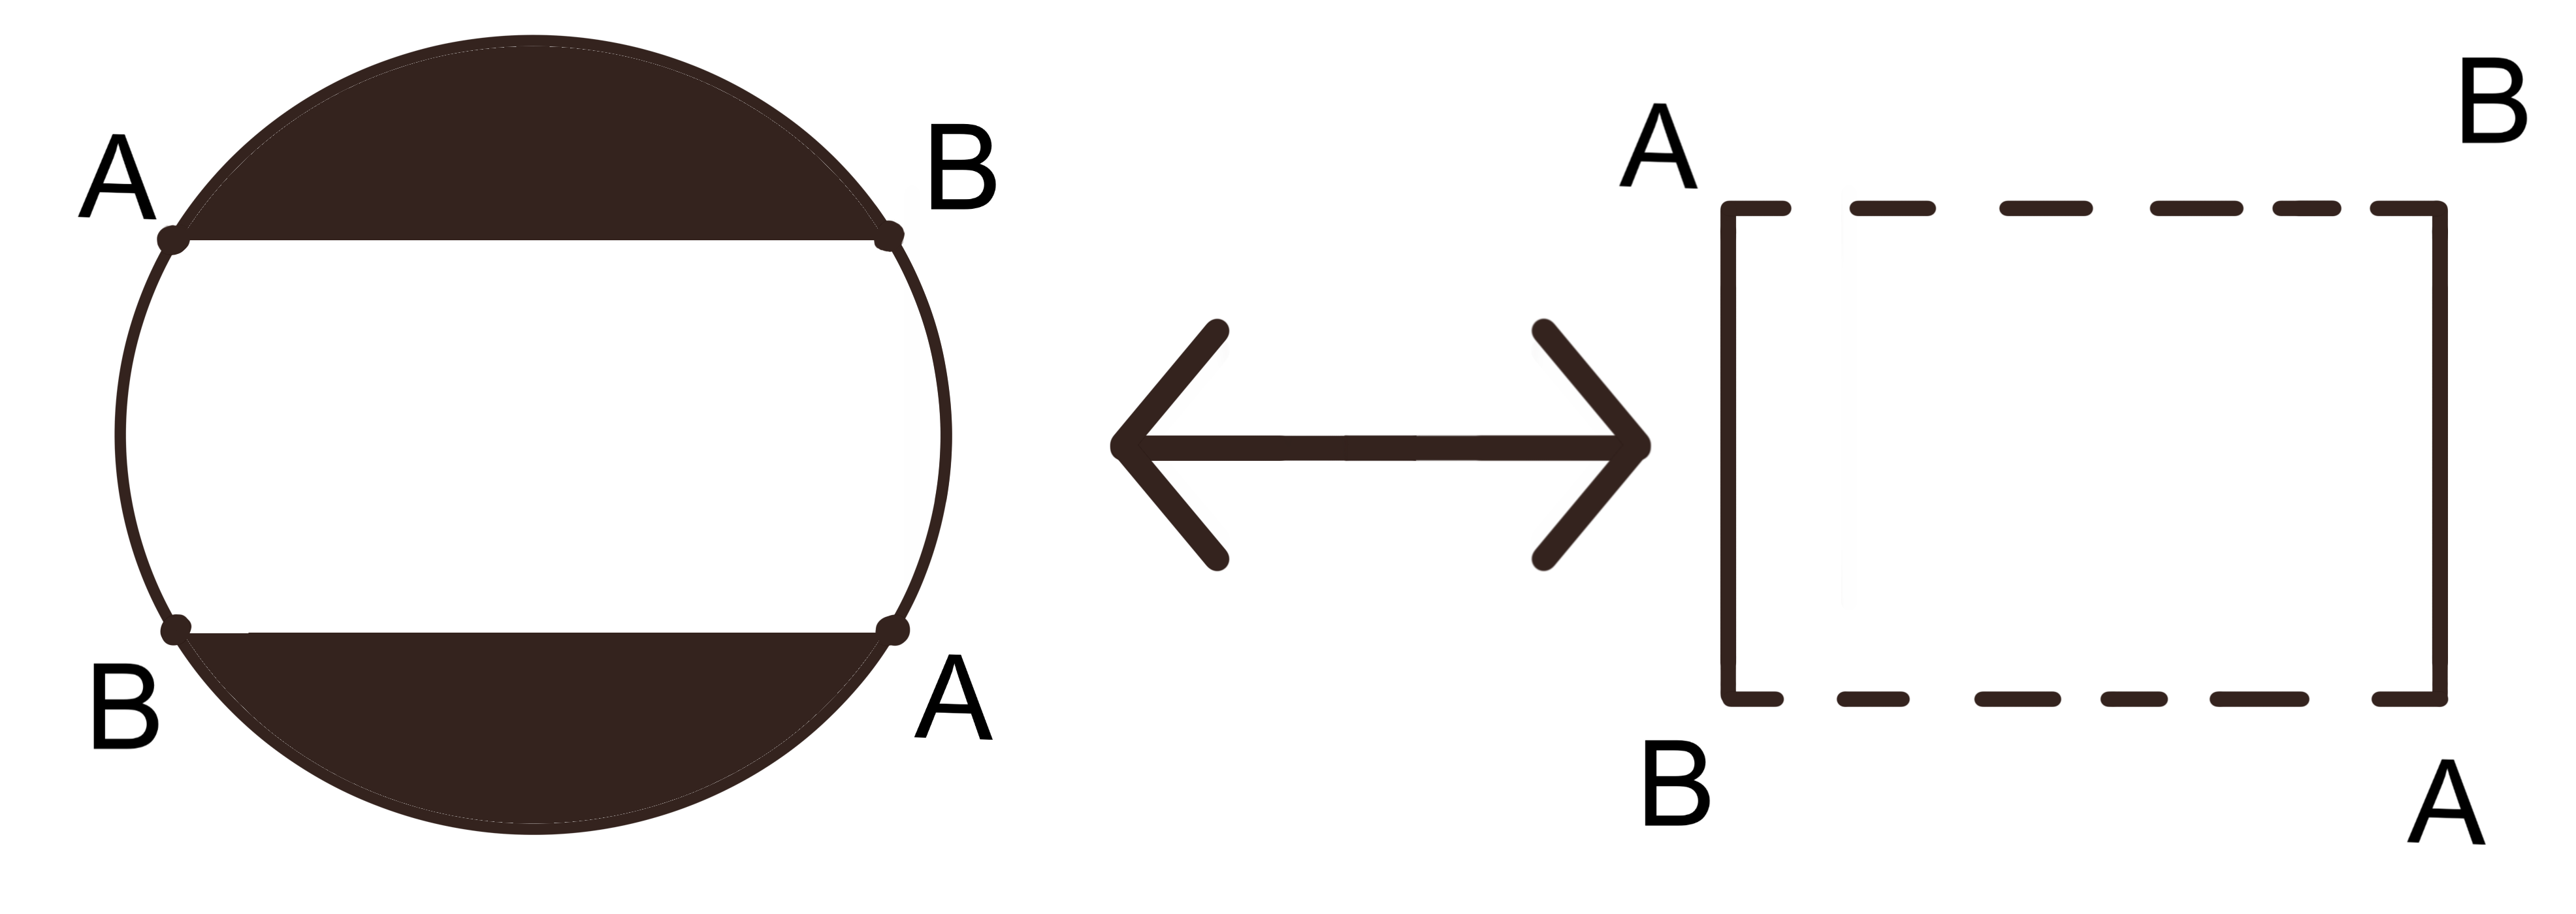
\includegraphics[width=0.4\linewidth]{imagenes/planop_sinD.png}
	\caption{Plano proyectivo menos un subconjunto homemorfo al disco cerrado}
	\label{fig:planop sin D}
\end{figure} 

Partiendo de dos planos proyectivos,  $I$ e $II$, retiramos el disco como en la figura \ref{fig:planop sin D}. Luego procedemos a identifcar ambos conjuntos como se indica en la figura \ref{fig:sumaconexadeppsEnLema}.

\begin{figure}[h!]
	\centering
	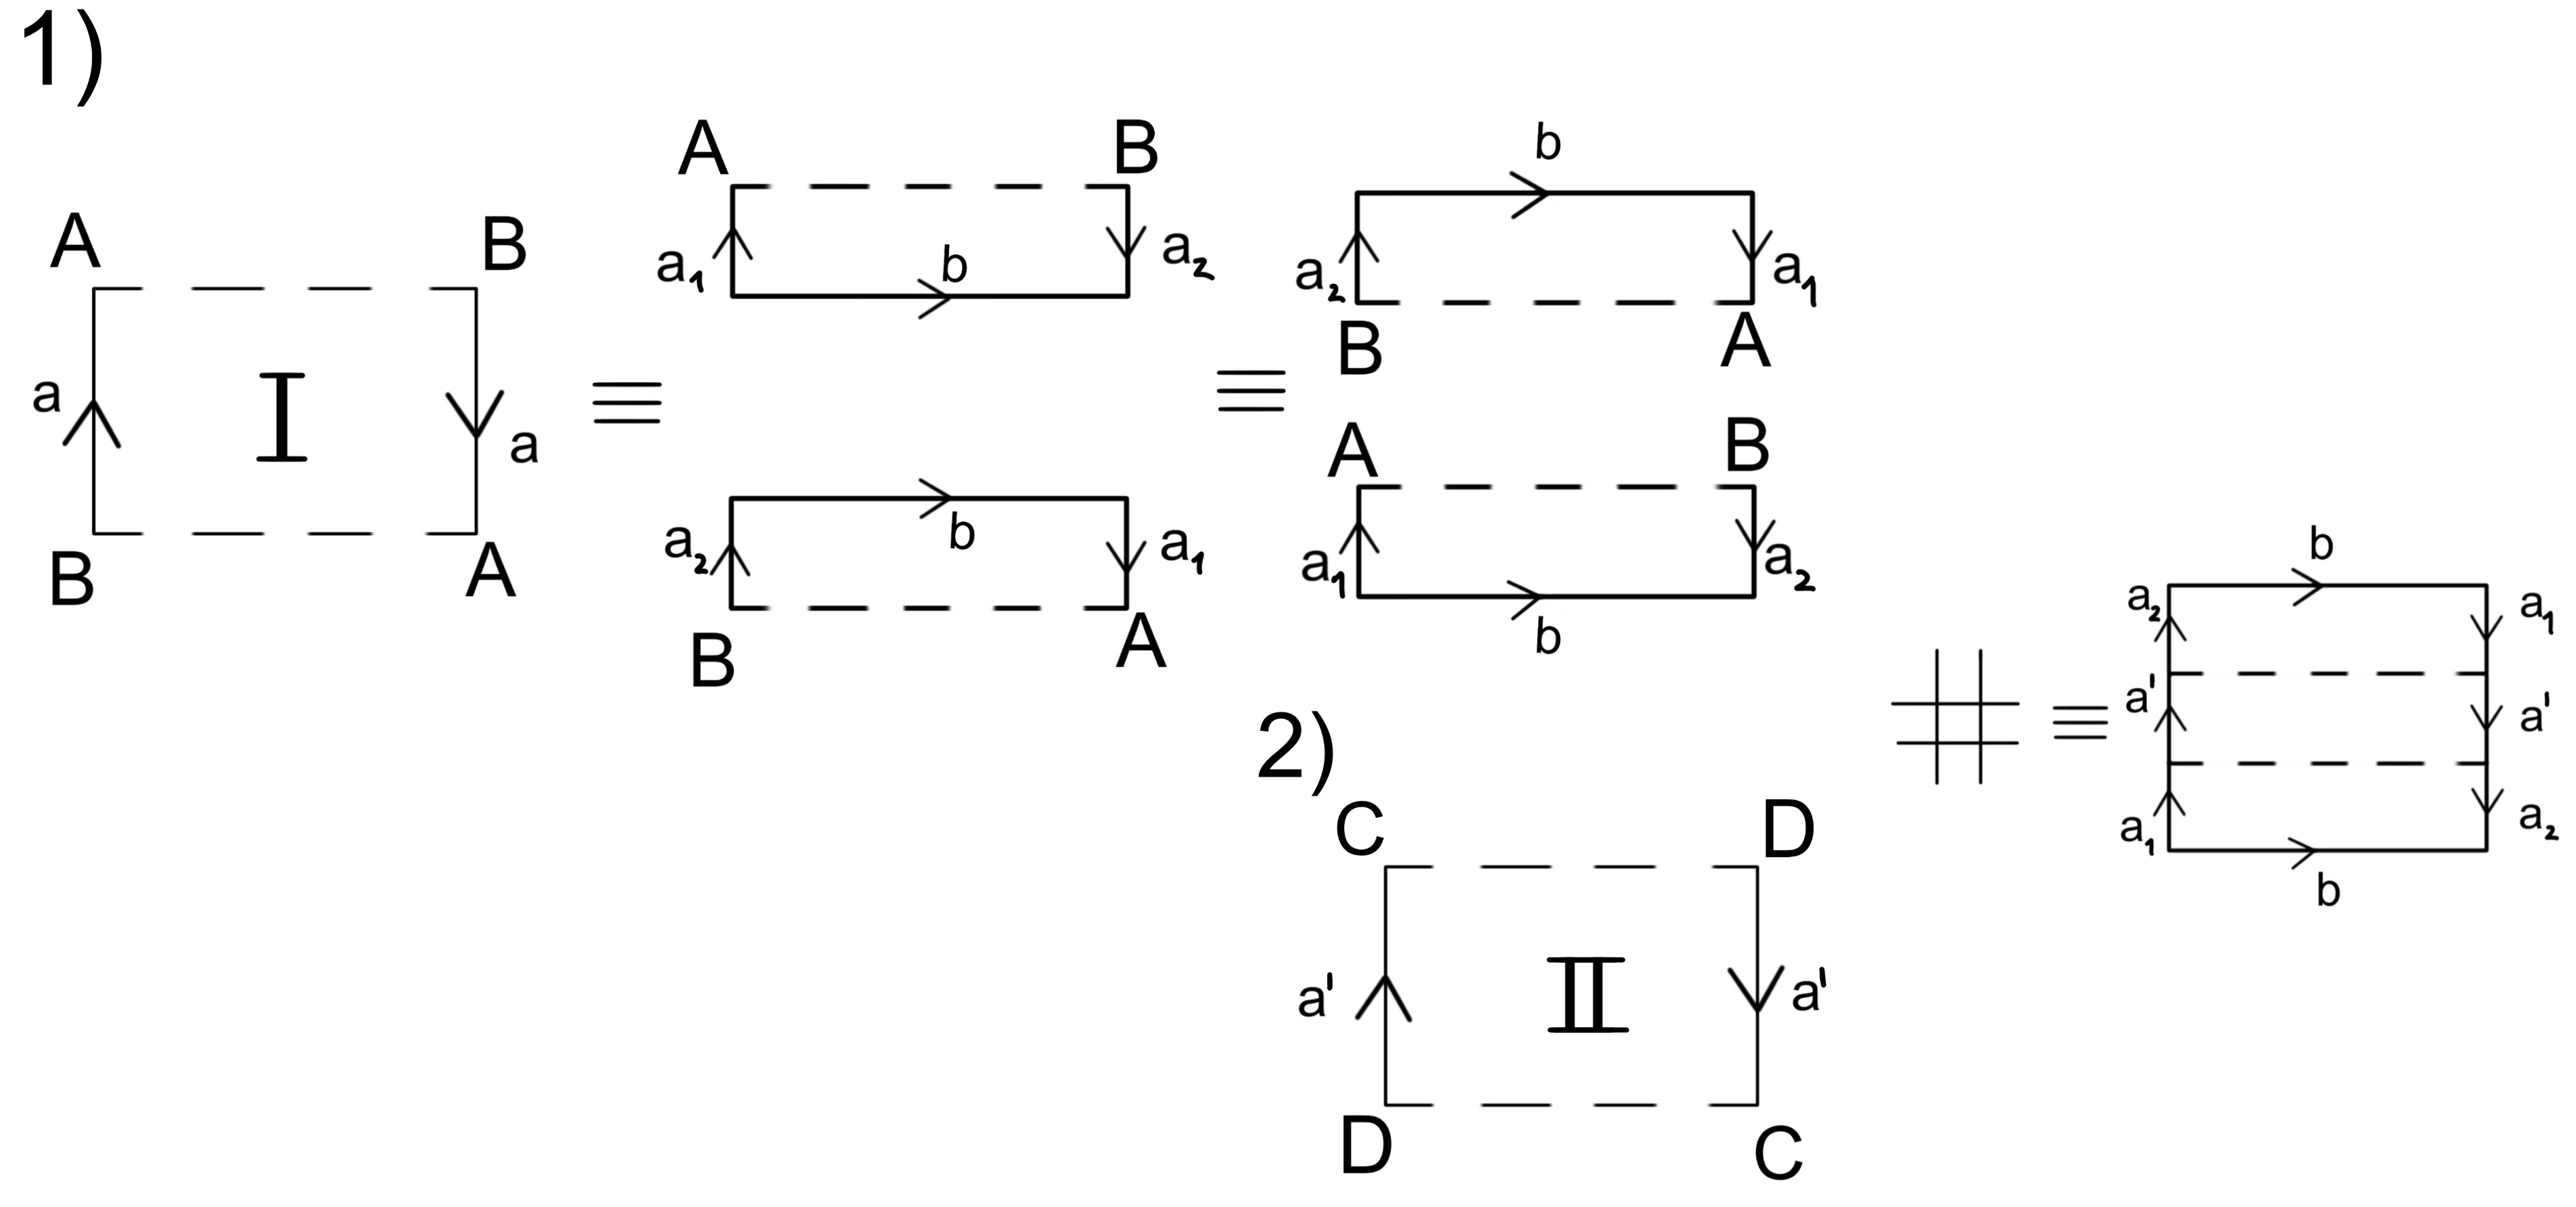
\includegraphics[width=0.8\linewidth]{imagenes/sumappsEnLema.png}
	\caption{Botella de Klein = $ I \# II$}
	\label{fig:sumaconexadeppsEnLema}
\end{figure} 

La figura final obtenida  es una Botella de Klein.
\end{proof}
\end{lema}

El ávido lector se habrá dado cuenta de un detalle de la demostración: retirar un disco de un plano proyectivo lo convierte en una banda de M\"obius!


\section{Triangulación de una superficie}
Una triangulación, en caso de existir, pretende expresar una superficie como un conjunto de triángulos identificados por las aristas. La noción de triangulación, \textit{a priori} inofensiva, será un ingrediente clave para poder manipular superficies compactas. Se define rigurosamente como:

\begin{defin}\label{defin:triangulacion}
Una \textbf{triangulación} de una superficie $S$, consiste en un conjunto de cerrados, $\{T_1, ..., T_n, ...\}$, que recubren a $S$ y en una familia de homeomorfismos, $\{\phi_1, ..., \phi_n, ...\}$, que cumplen:

\begin{align*}
	\phi_i: T'_i \longrightarrow T_i
\end{align*}

Donde $T'_i$ es un triángulo del plano $\mathbb{R}^2$.
Además, se exige que para cualesquiera dos $T_i$ y $T_j$ con $i\neq j$, se cumpla una de las siguientes condiciones: o son conjuntos totalmente disjuntos; o comparten un vértice en común y solo eso; o tienen toda una arista en común y solo eso.\\
Adicionalmente, llamaremos \textbf{vértice} a todo elemento de $S$ que se corresponde por algún $\phi_i$ con un vértice en el plano. Y llamaremos \textbf{arista} a todo subconjunto de $S$ que tenga por imagen una arista de algún $T'_i$.\\
\textbf{Observación:} En el caso de superficies compactas, a la triangulación se le exige estar compuesta por un número finito de triángulos.
\end{defin}


Intuitivamente, podemos pensar en una triangulación como una teselación por triángulos de una superficie dada. Estudiemos algunos ejemplos concretos para familiarizarnos con el concepto:

El toro se puede triangular como ilustra la figura  \ref{fig:toro triangulado}. Fijémonos que basta con definir una lista de triángulos, con sus respectivos vértices, para concretar una trinagulación. En la figura indicada la lista sería:
[Lista de triángulos]

\begin{figure}[h!]
	\centering
	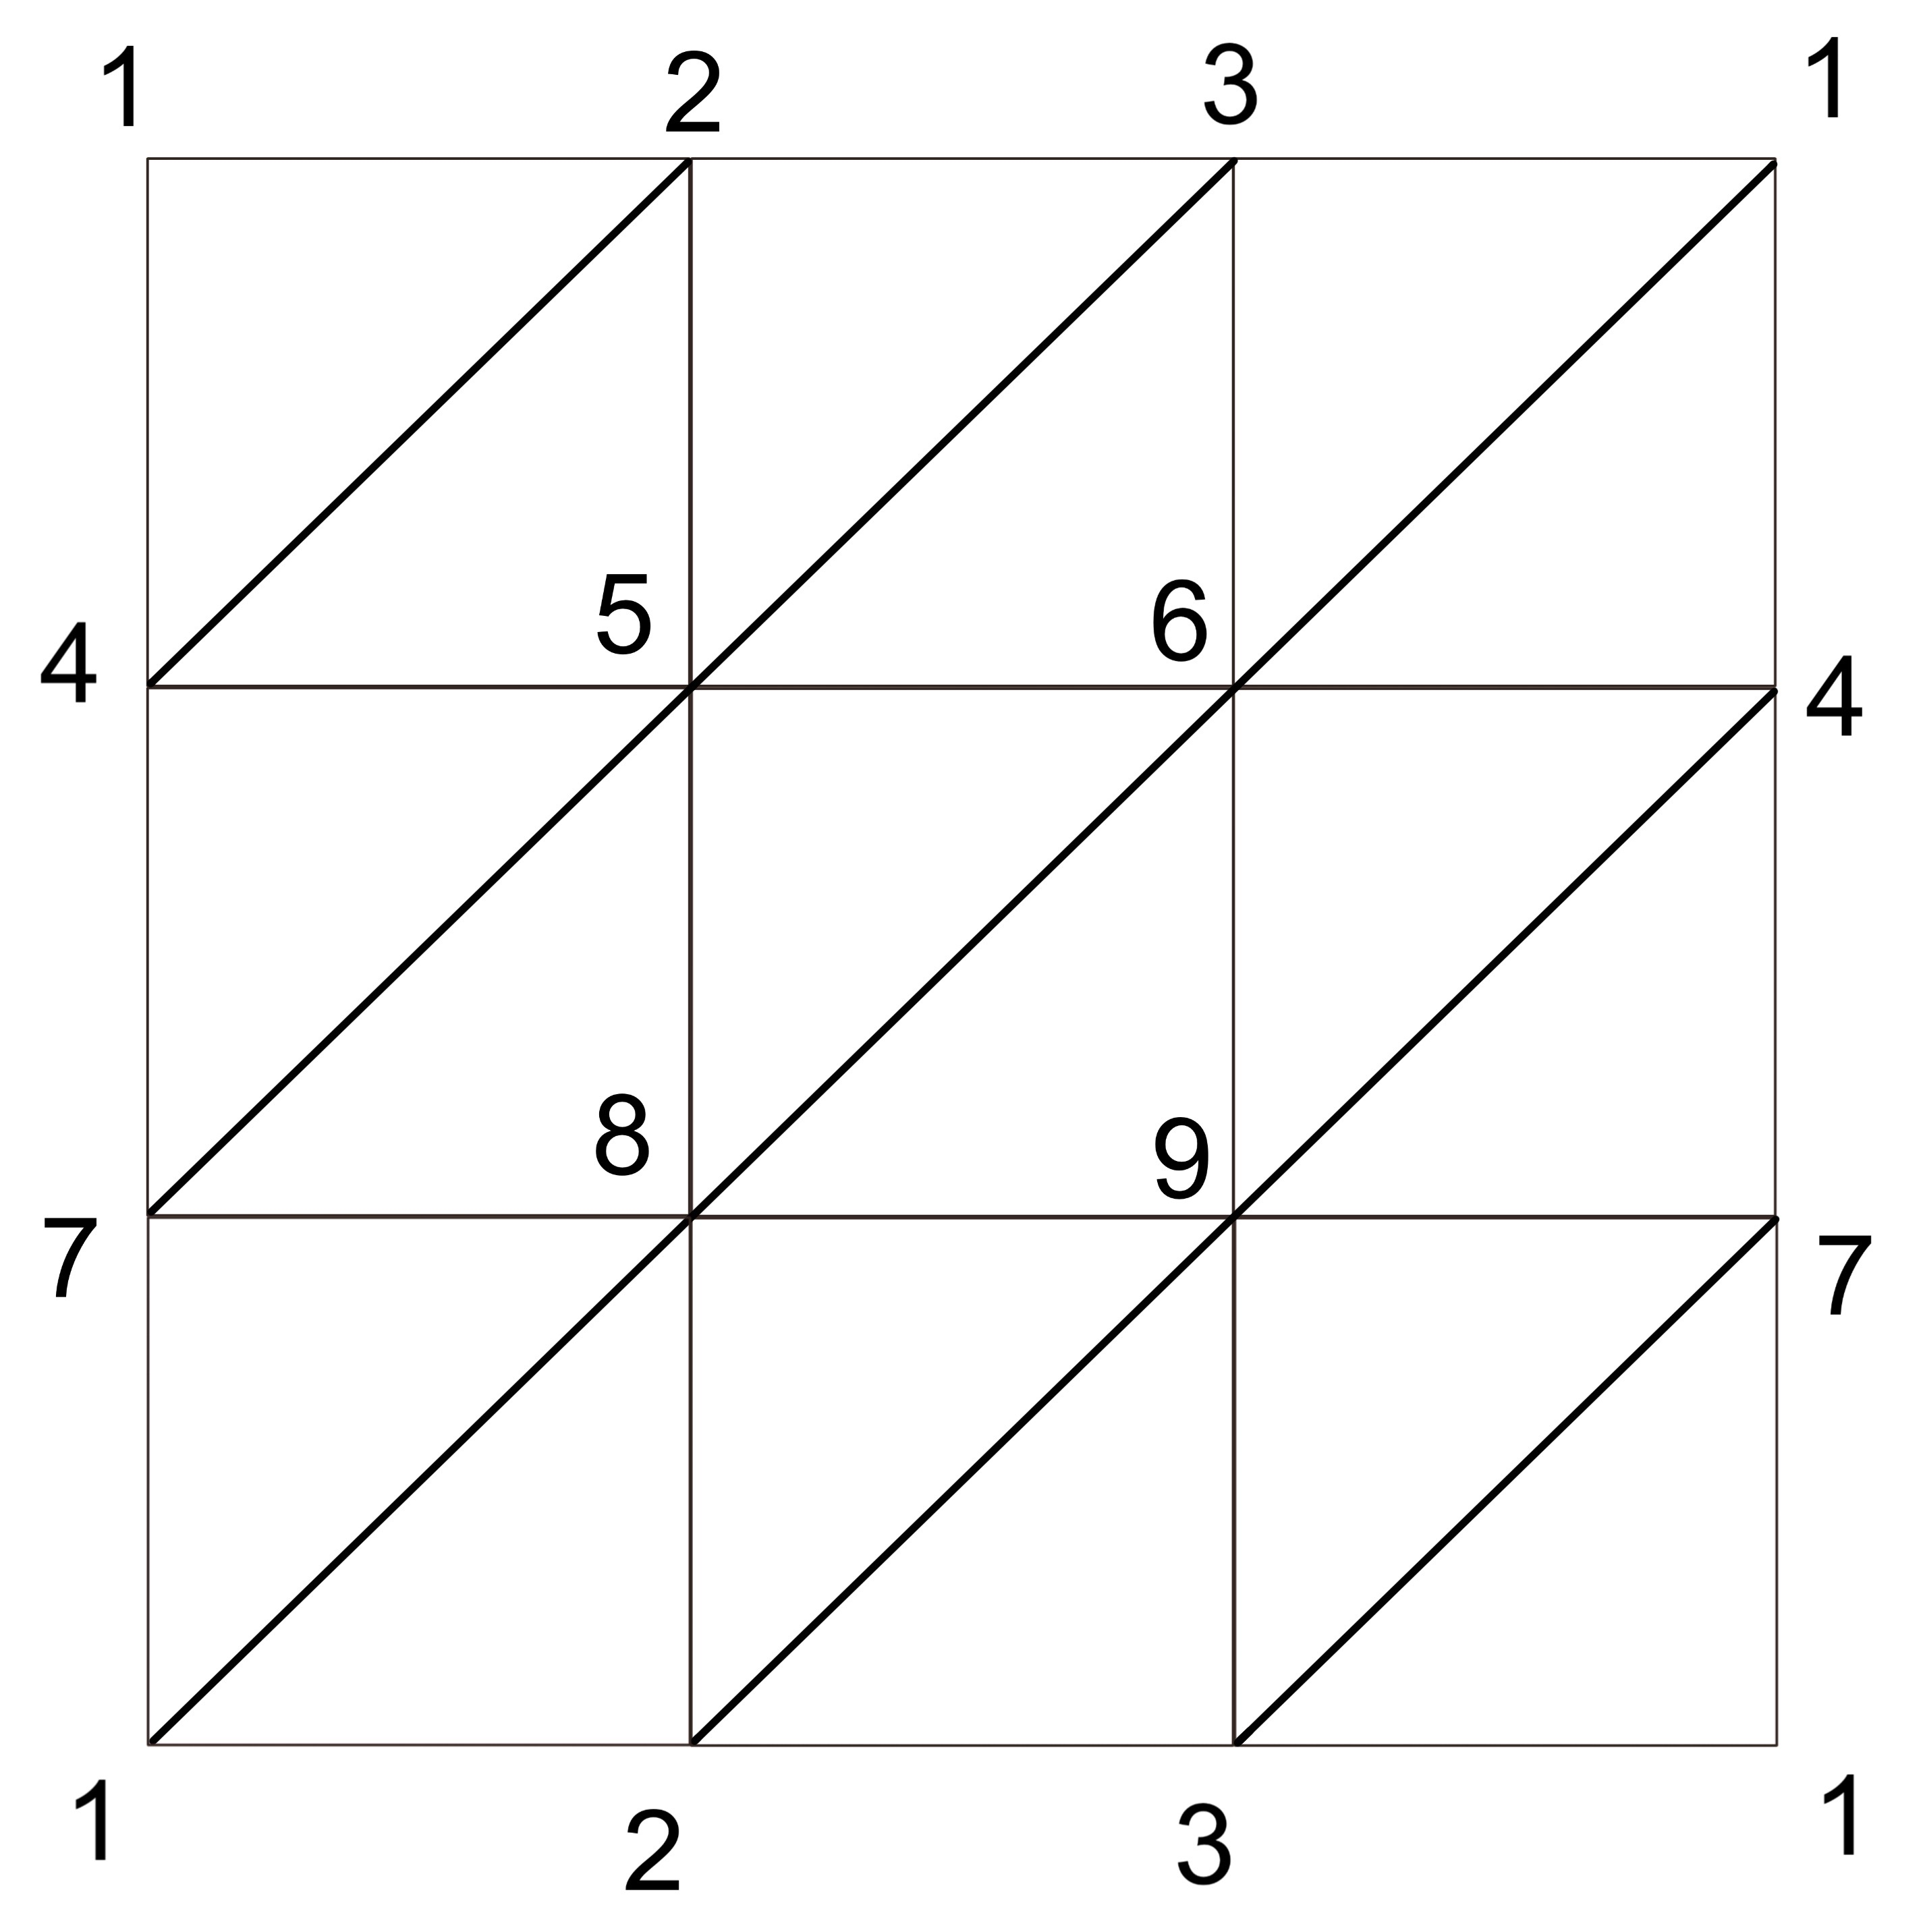
\includegraphics[width=0.3\linewidth]{imagenes/toro_triangulado.png}
	\caption{Triangulación del toro}
	\label{fig:toro triangulado}
\end{figure} 

En la figura \ref{fig:no triangulaciones} señalamos un par de intentos de simplificar la triangulación del toro. Sin embargo, notemos que ninguna de las dos imágenes son triangulación del toro. La primera, aunque triangulación, no es homeomorfa al toro; La segunda ni siquiera satisface las condiciones de triangulación.

\begin{figure}[h!]
	\centering
	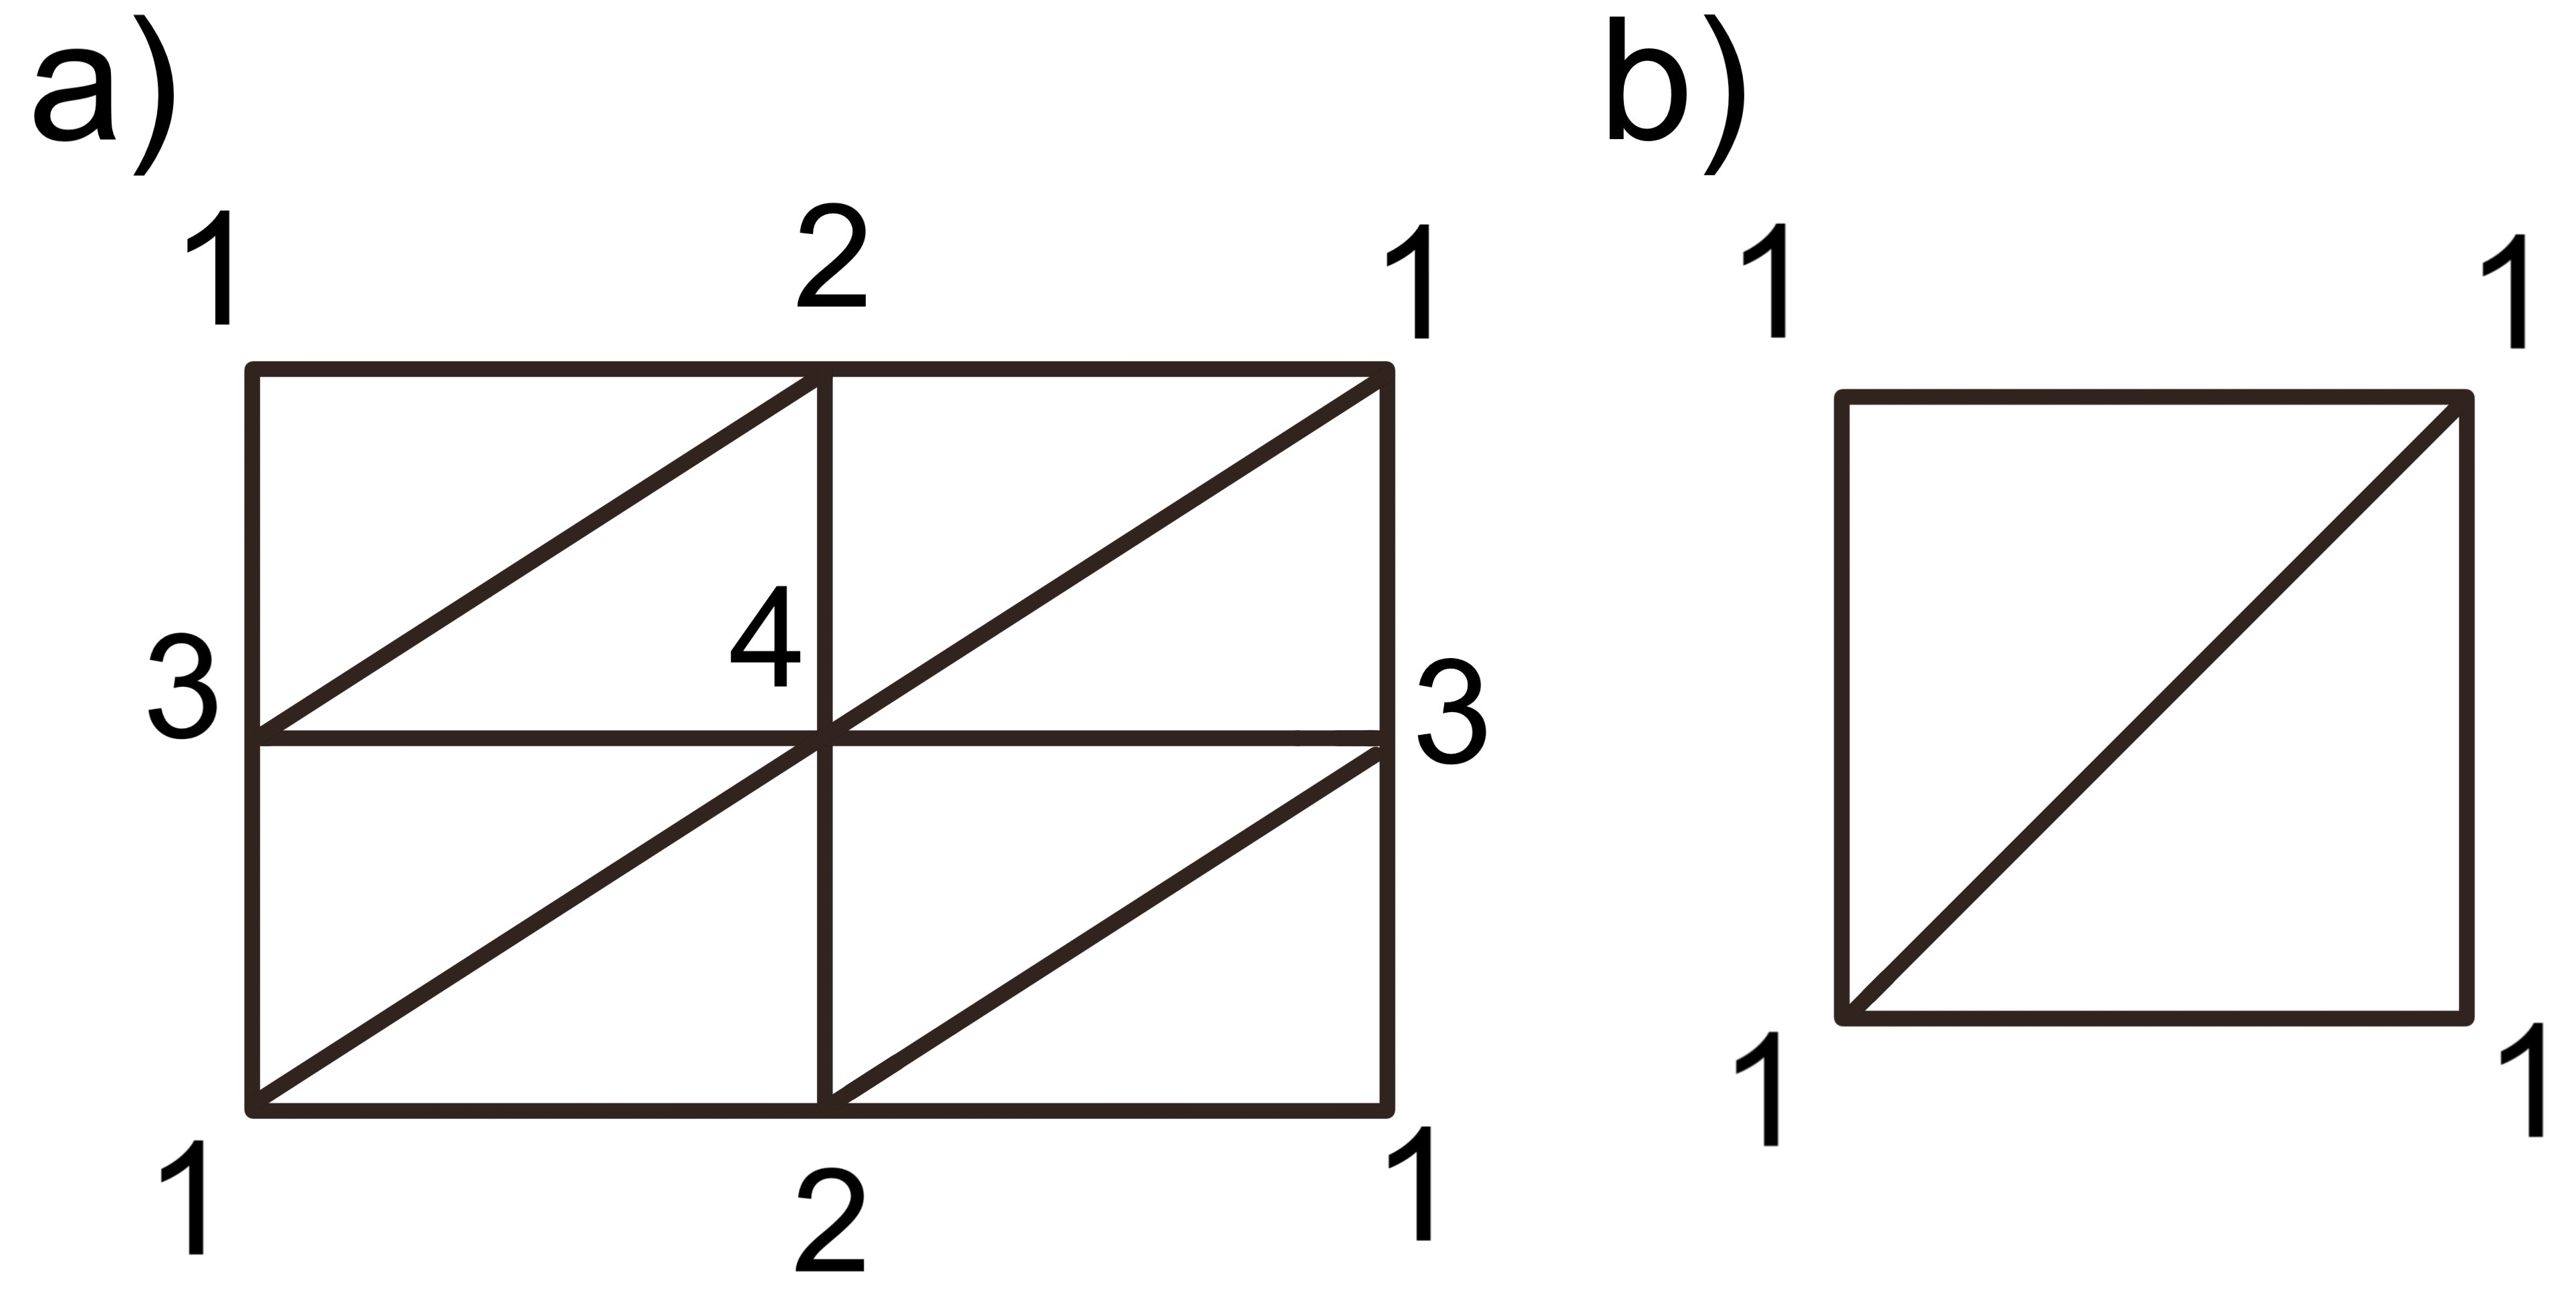
\includegraphics[width=0.5\linewidth]{imagenes/no_triangulaciones.png}
	\caption{Ejemplos de cosas que no son triangulaciones}
	
	\label{fig:no triangulaciones}
\end{figure} 

Para el caso del plano proyectivo, se propone en la figura \ref{fig:plano proyectivo triangulado} una triangulación.

\begin{figure}[h!]
	\centering
	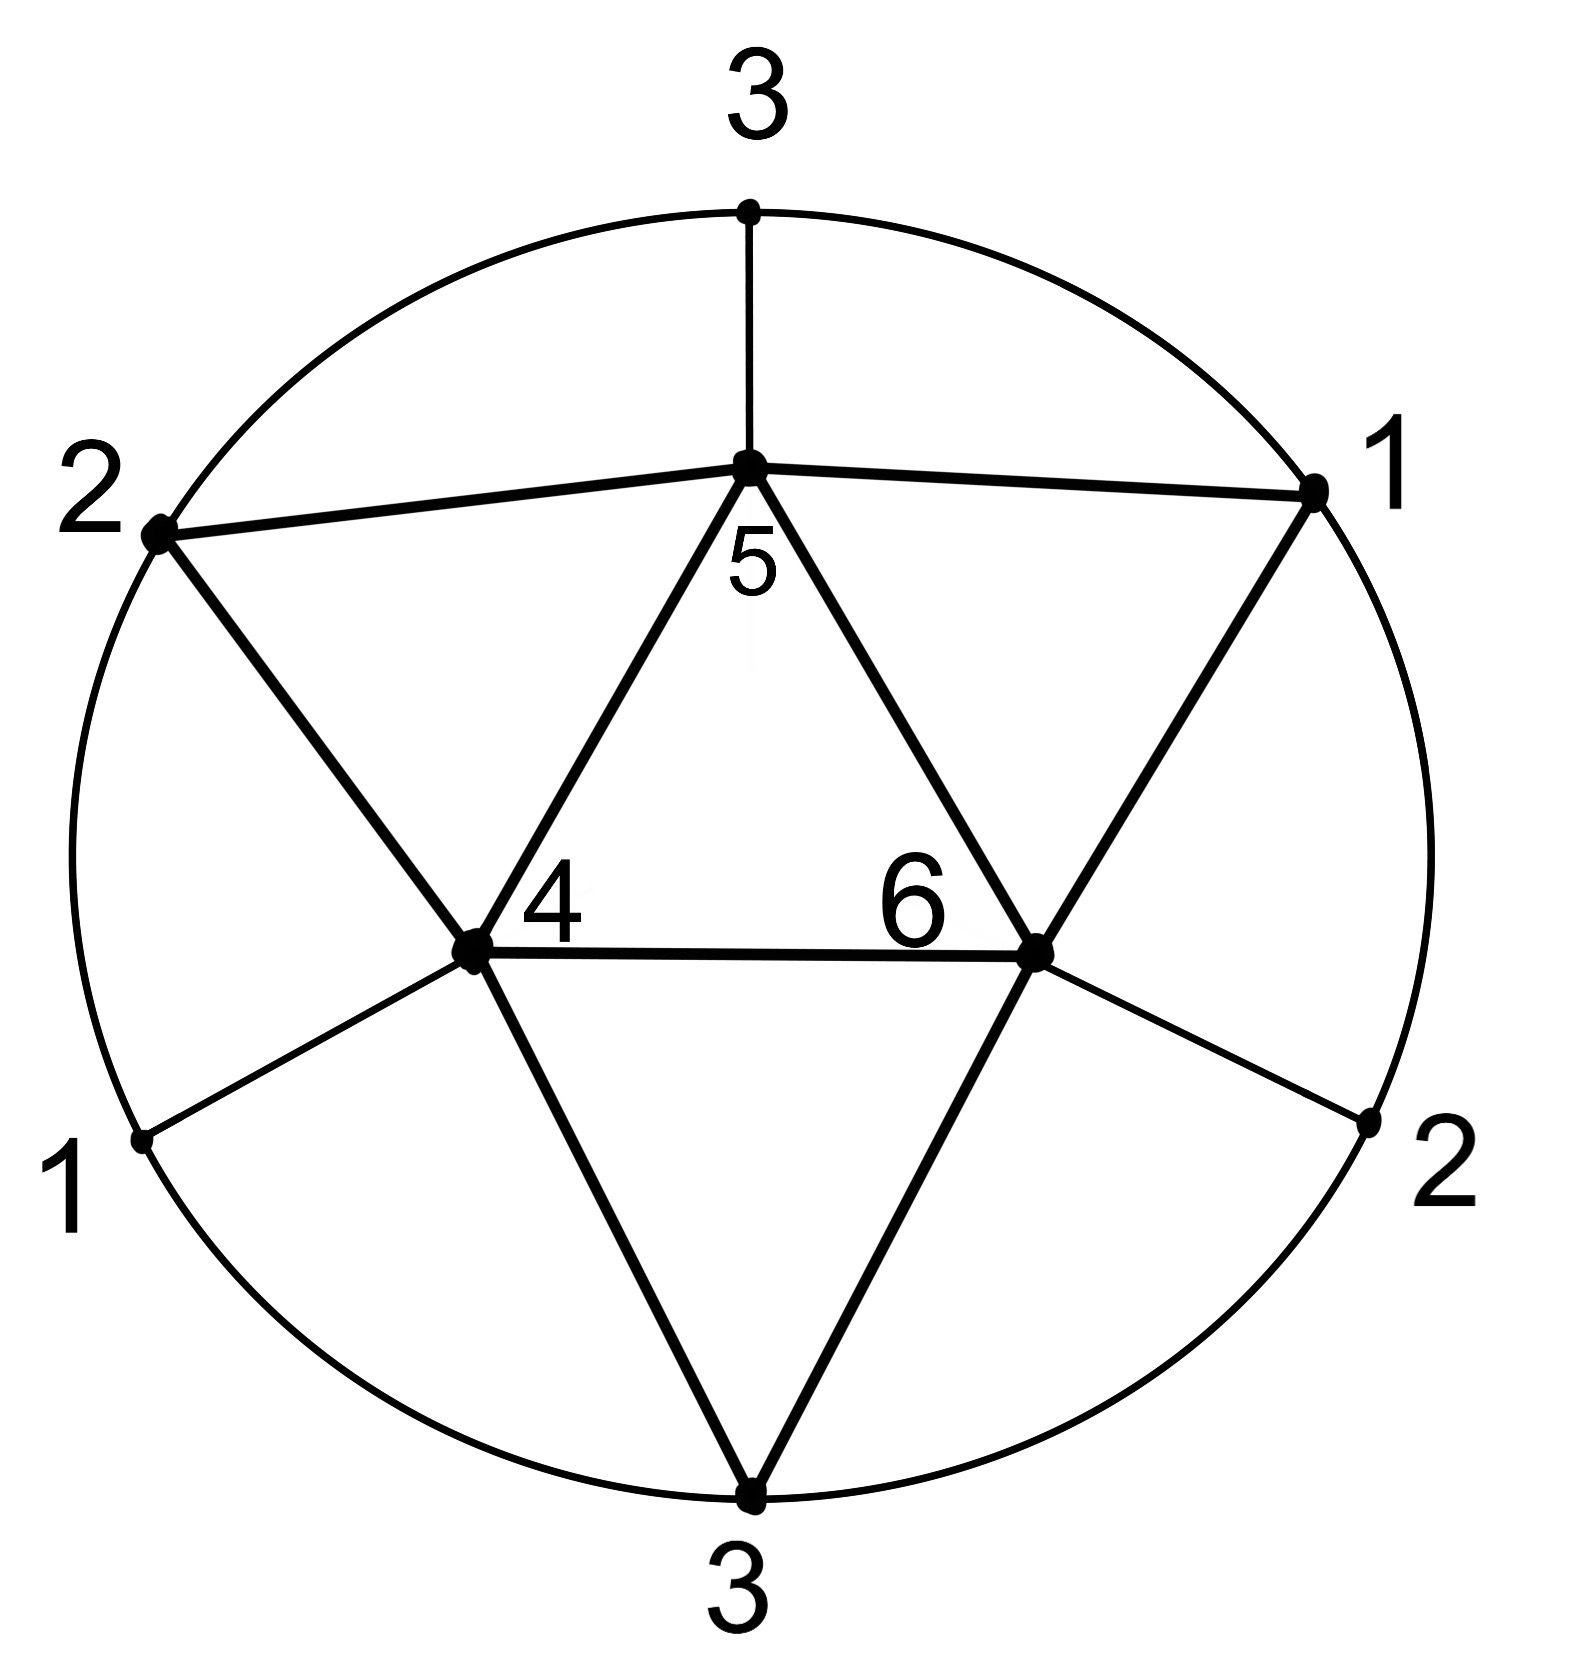
\includegraphics[width=0.3\linewidth]{imagenes/planop_triangulado.png}
	\caption{Triangulación del plano proyectivo}
	\label{fig:plano proyectivo triangulado}
\end{figure} 


\subsection*{Resultados sobre la triangulación}

Primero, veamos un par de lemas que nos enmarcan el comportamiento de las triangulaciones:

\begin{lema}\label{lema:lema1detriangulacion}
Sea $S$ una superficie triangulable entonces una arista lo es de exactamente dos triángulos.

\begin{proof}
Supongamos que una arista lo es de uno o más de dos triángulos. Elegimos un $x\in S$ de dicha arista. Por un lado, sabemos que un entorno de $x$ es homeomorfo a 
\[U^2 = \{x\in\reales^2: ||x||<1\}\]
Por otra parte, veamos los distintos casos:

\begin{enumerate}
\item[(a)] Si la arista lo fuese de un único triángulo, entonces tendríamos entornos de $x$ homeomorfos a
\[ H^2 = \{(x,y)\in\reales^2: x^2+y^2<1, \, y\geq 1 \} \]

\item[(b)] Si la arista lo fuese de  $n$ triángulos, con $n\geq 3$. Entonces tendríamos entornos de $x$ homeomorfos a pegar $n$ conjuntos de la forma de $H^2$ (podemos hacerlos disjuntos trasladándolos). Más rigurosamente, el conjunto a cocientar sería
\[
   \bigcup^n_{i=1} \{(x+10i,y)\in\reales^2: (x-10i)^2+y^2<1, \, y\geq 1 \} \}	        
\]
Identificando los puntos con $y=0$. En la figura \ref{fig:tripleplano} ilustramos el caso para $n=3$.
\end{enumerate}    

En cualquier de los dos casos estaríamos incurriendo en un absurdo, con lo que concluimos la demostración.
\end{proof}
\end{lema}

\begin{figure}[h!]
	\centering
	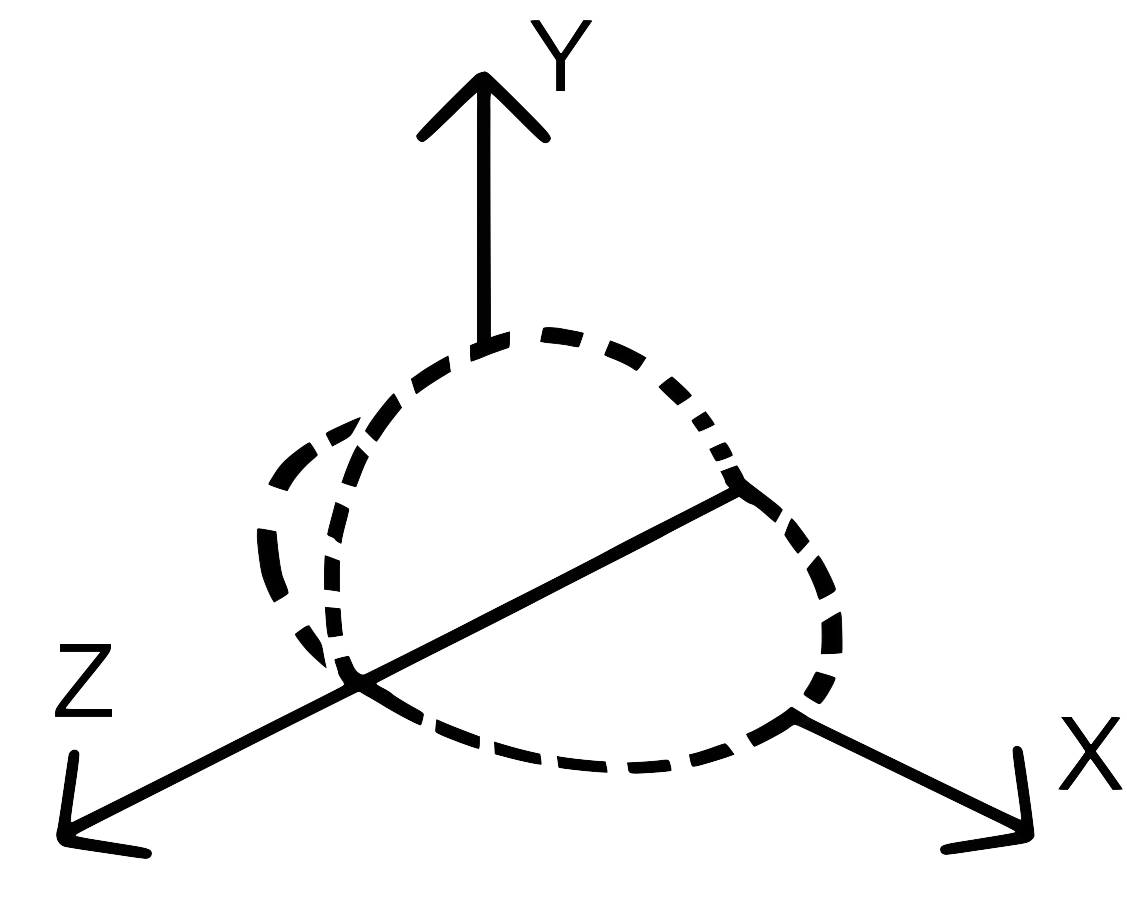
\includegraphics[width=0.4\linewidth]{imagenes/tripleplano.png}
	\caption{Identificación por la frontera de $H^2$}
	\label{fig:tripleplano}
\end{figure}

\begin{lema}\label{lema:lema2detriangulacion}
Sea  $S$ una superficie triangulable y $v\in S$ un vértice en esa triangulación, entonces podemos ordenar el conjunto de todos los triángulos con vértice $v$ cíclicamente,  $T_0, T_1, ..., T_n = T_0$, de manera que $T_i$ y $T_{i+1}$ tienen toda una arista en común para todo $0\leq i\leq n-1$.

\begin{proof}
Fijado un vértice $v$, podemos utilizar el lema anterior (\ref{lema:lema1detriangulacion}) para hacer una partición del conjunto de triángulos que tienen a $v$ por vértice. Si ocurriese que hay más de un conjunto disjunto en la partición, entonces $v$ no podría tener un entorno homeomorfo a $U^2$.
\end{proof}

\end{lema}

La idea de triangulación compone una herramienta potente para el manejo de superficies en general. Sin embargo, para usarla primero es necesario probar que \textit{de facto} existe una tal triangulación. Por suerte, el siguiente resultado del matemático Tibor Radó nos garantiza su existencia. Enunciamos el teorema sin, lamentablemente, dar demostración.

\begin{teor}{Teorema de triangulación}\label{teor:teoremaDeTriangulacion}	

Toda superficie separable es triangulable.
\end{teor}
En el contexto de este trabajo, las superficies son segundo numerables por definición. Por tanto, todas las superficies son separables y con ello triangulables.

Con este teorema concluimos el arsenal de herramientas que nos hará falta para emprender la demostración del teorema de clasificación de superficies compactas.





\chapter{Clasificación de superficies compactas}

\begin{teor}{Teorema de clasificación de superficies compactas}\label{teor:teoremadeclasificacion}	
Toda superficie compacta es homeomorfa a una esfera, a una suma conexa de toros o una suma conexa de planos proyectivos.
\end{teor}

\subsubsection*{Idea de la demostración}
El primer paso de la demostración será probar que podemos tratar cualquier superficie compacta como un polígono en $\reales^2$ con sus aristas identificadas a pares. Para esta parte de la demostración nos serviremos del teorema \ref{teor:teoremaDeTriangulacion} de \textit{T. Radó}.\\
Posteriormente, utilizando la representación en $\reales^2$, iremos modificando la figura con transformaciones homeomorfas. A cada transformación iremos simplificando el polígono que se obtiene. Tras aplicar todos los pasos, comprobaremos que el polígono final corresponderá con una de las expresiones canónicas introducidas en la sección \ref{subsec:expresionescanonicassumasconexas}. Para conseguir este resultado final nos hará falta el lema \ref{lema:planop+toro=3planop} demostrado en el anexo, este resultado nos garantiza que la suma conexa de un plano proyectivo y un toro es homeomorfa a la suma de tres planos proyectivos.\\
Habiendo llegado a las expresiones canónicas de \ref{subsec:expresionescanonicassumasconexas}, habremos concluido que la superficie inicial es homeomorfa o a una esfera, o a una suma conexa de toros, o a una suma conexa de planos proyectivos.\\

\section{Primer paso}
Buscamos demostrar que cualquier superficie compacta $S$ es homeomorfa un polígono $\reales^2$ con sus aristas identificadas a pares.

Por el teorema \ref{teor:teoremaDeTriangulacion} tenemos que $S$ es triangulable. Sean $T_1, T_2, ..., T_n$ los triángulos de S y sean $T'_1, T'_2, ...,  T'_n$ los correspondientes triángulos en $\reales^2$, tenemos los homeomorfismos:
\[ \phi_i: T'_i \longrightarrow T_i \]
Podemos asumir que los $T'_i$ son disjuntos (en caso de que no lo fueran, bastaría con componer con una traslación). Además, podemos organizar los triángulos de forma tal que todo $T_i$ tiene al menos una arista $e_i$ en común con algún tríangulo $T_1, ..., T_{i-1}$ para $2\leq i \leq n$; para ello elegimos $T_2$ que tenga una arista en común con $T_1$, elegimos $T_3$ que tenga una arista en común con $T_1$ o $T_2$, y así sucesivamente. Si en algún punto no pudiésemos elegir un $T_k$, tendríamos entonces dos conjuntos disjuntos $\{T_1, ..., T_{k-1} \}$ y $\{T_k, ..., T_n\}$, pero esto dividiría a $S$ en dos conjuntos cerrados disjuntos contradiciendo la hipótesis de conexión.\\
Sea $T' = \bigcup T'_i$, definimos la función 
\[ \phi: T' \longrightarrow S \]
como $\phi |_{T'_i} = \phi_i$ para todo $i$. La función $\phi$ es sobreyectiva y continua\footnote{Para probar la continuidad basta con escribir cualquier abierto en $S$ como unión finita de la partición de triángulos.}. Al ser $T'$ compacto y $S$ Hausdorff, entonces $\phi$ es cerrada, de lo que se sigue que $S$ tiene la topología cociente inducida por $\phi$.

El polígono que queremos construir será descrito como espacio cociente de $T'$. Por hipótesis, tenemos que $e_i$ es arista de los triángulos $T_i$ y $T_j$ para algún $1\leq j < i$, y a su vez $\phi^{-1}(e_i)$ es arista de $T'_i$ y $T'_j$. Identificamos ambos triángulos en $T'$ a lo largo de la arista $\phi^{-1}(e_i)$. El mismo procedimiento se puede aplicar para las aristas $e_2, e_3, ..., e_n$, obteniendo como resultado un conjunto cociente $D$ del conjunto inicial $T'$. La función $\phi$ induce una nueva función continua $\psi: D \longrightarrow S$. De nuevo, al ser $D$ compacto y $S$ Hausdorff, tenemos que $\psi$ es   cerrada y con ello que $S$ tiene la topología cociente inducida por esta función. \\
Veamos que $D$ es homeomorfo al disco cerrado $E^2 = \{x\in \reales^2: ||x||\leq 1\}$:

\begin{enumerate}
\item[(a)] Tenemos que el triángulo $T'_i$ en $\reales^2$ es homeomorfo a $E^2$.

\item[(b)] Dados dos discos cerrados $E^2_1$ y $E^2_2$, si los identificamos por un segmento cerrado de sus fronteras, obtenemos un espacio cociente homeomorfo, de nuevo, a un disco cerrado. De aquí se sigue que, si tenemos dos triángulos $T'_i$ y $T'_j$  identificados por una de sus aristas, entonces el espacio resultante es homeomorfo a $E^2$.
\end{enumerate}
Utilizando (a) y (b) tenemos que el espacio cociente $D$ obtenido a partir de $T'$, es topológicamente equivalente a un disco cerrado. Además, sabemos que el espacio cociente que induce $\psi$ coincidirá  con el disco cerrado en el cual segmentos de su frontera están identificados a pares; esto se sigue del proceso de construcción de $D$, teniendo en cuenta que al identificar la arista $\phi^{-1}(e_i)$ de dos triángulos, el resto de aristas en la frontera siguen emparejadas (sabemos que van por parejas por el lema \ref{lema:lema1detriangulacion}).


En la figura \ref{fig:tetraedrotriangulado} tenemos un tetraedro triangulado

\begin{figure}[h!]
	\centering
	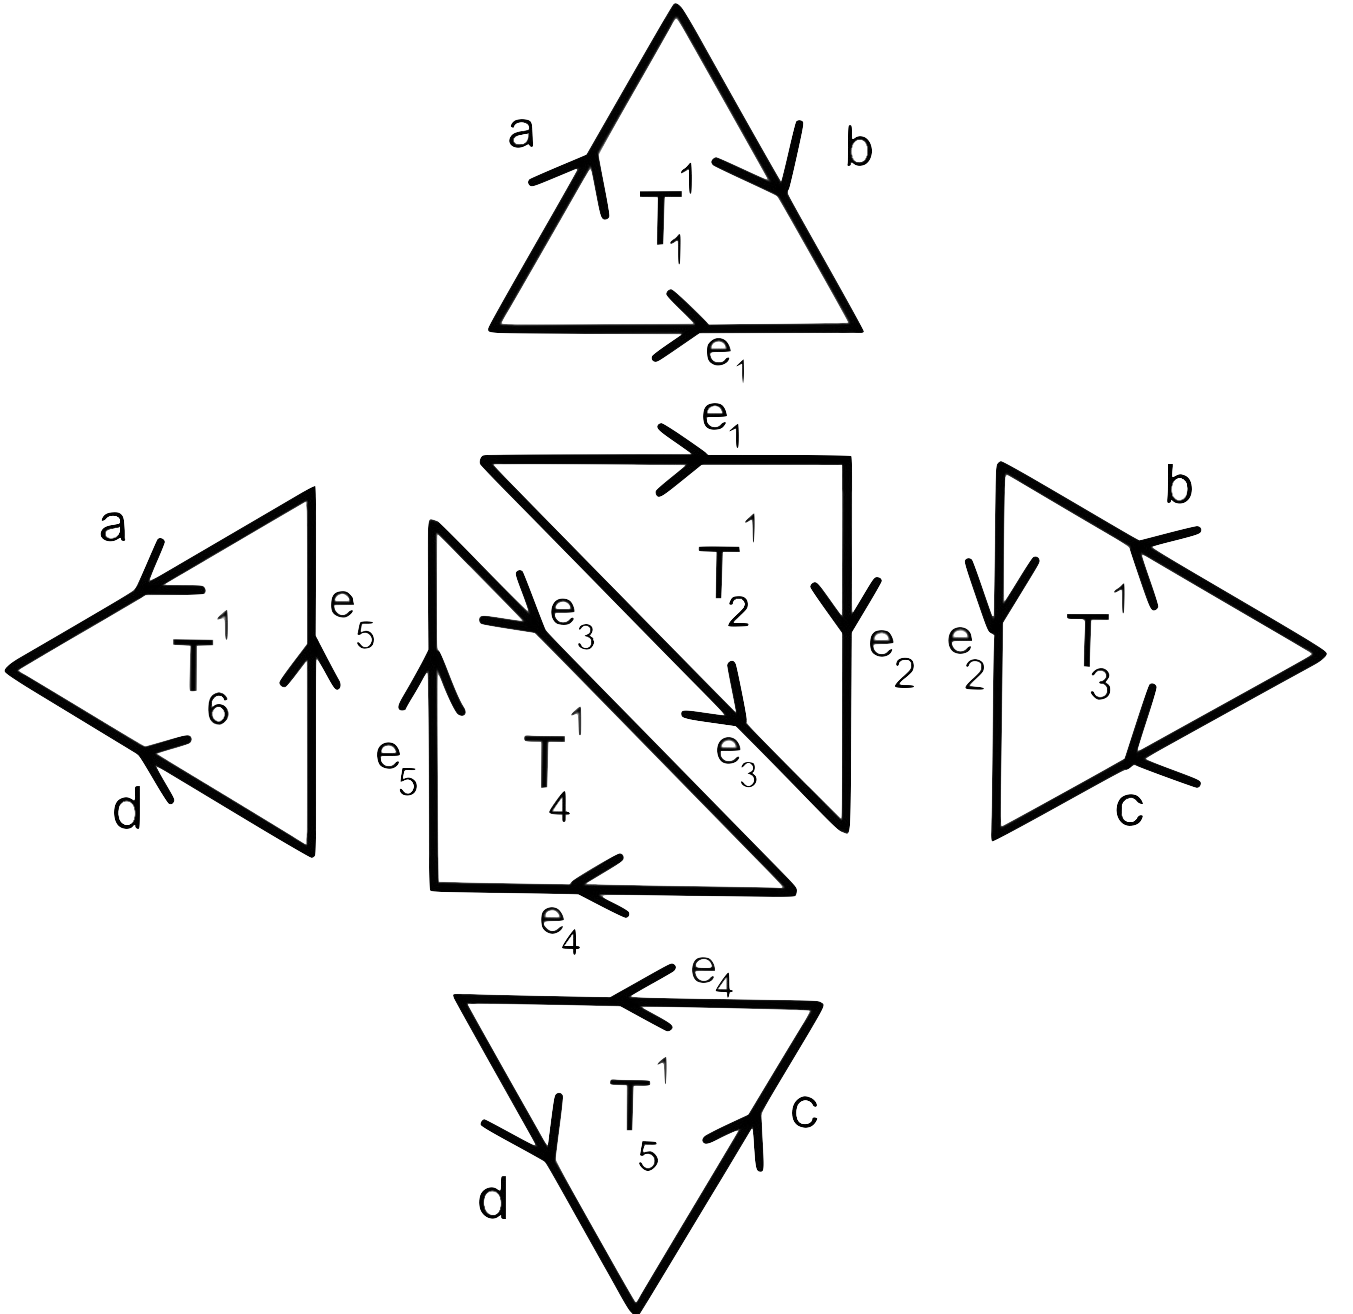
\includegraphics[width=0.3\linewidth]{imagenes/tetraedro.png}
	\caption{Tetraedro triangulado}
	\label{fig:tetraedrotriangulado}
\end{figure}

Ilustramos en la figura \ref{fig:d} cómo se representaría el mismo tetraedro como el espacio cociente $D$ descrito en esta sección.

\begin{figure}[h!]
	\centering
	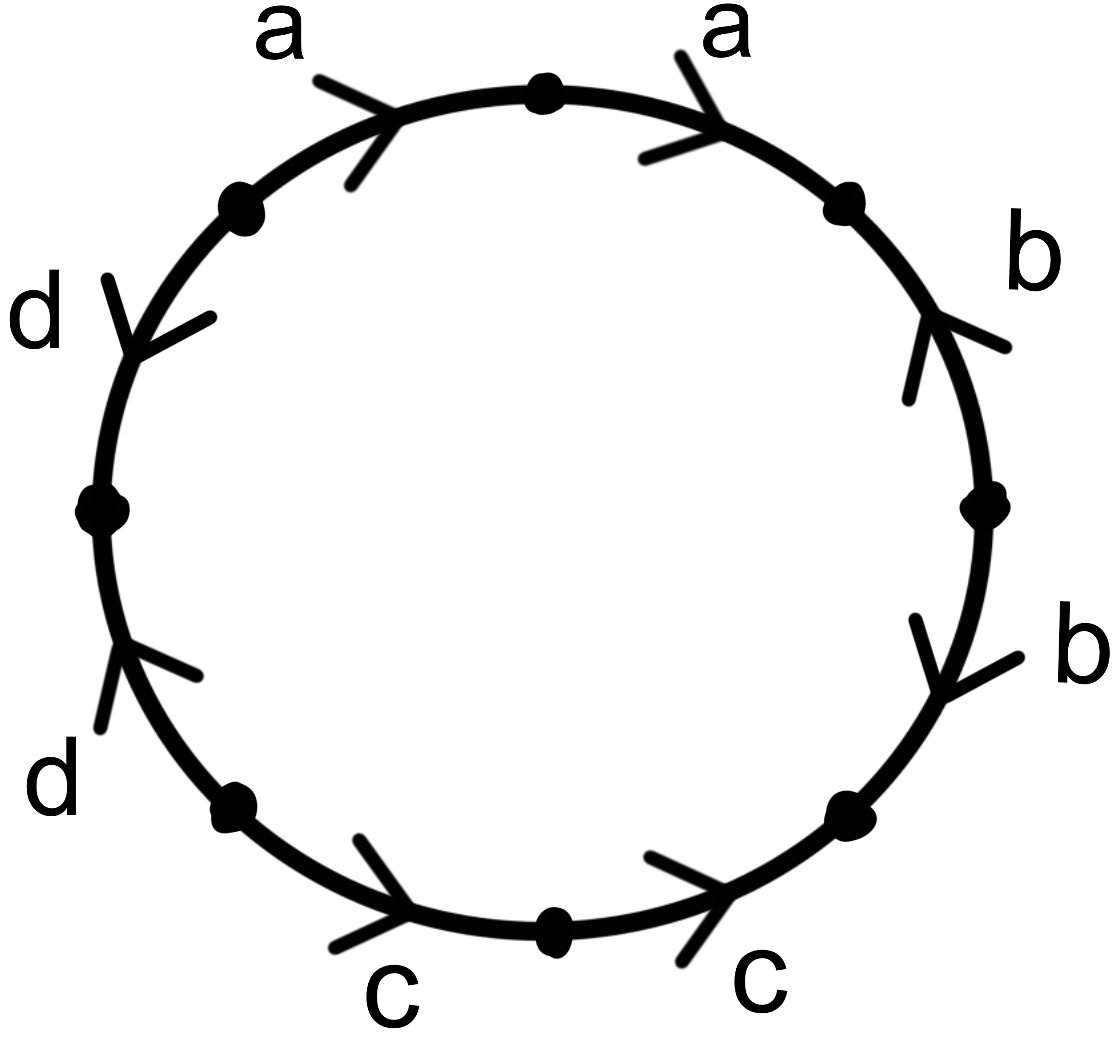
\includegraphics[width=0.3\linewidth]{imagenes/d.jpeg}
	\caption{Tetraedro como espacio cociente de un disco}
	\label{fig:d}
\end{figure}

A partir de aquí, manipularemos la superficie compacta $S$ como si de un polígono se tratase. Asumiendo que las aristas del polígono están identificadas a pares y sin ningún orden ni dirección particular.


\section{Segundo paso}

El segundo paso consiste en la eliminación de aristas adyacentes de primera especie.

Del primer paso hemos obtenido el polígono $D$ que representa a la superficie $S$ si se identifican sus aristas a pares. El polígono identificado lo podemos expresar con la misma notación que usamos para las expresiones canónicas (véase la sección \ref{subsec:expresionescanonicassumasconexas}). Por ejemplo, en el caso de la figura \ref{fig:d}, podemos expresarlo como:
\[ a^{-1}abb^{-1}cc^{-1}d^{-1}d \]
Si en esta expresión un par de aristas con el mismo símbolo aparecen  con exponentes +1 y -1 ($...a...a^{-1}$, por ejemplo), entonces diremos que el par es de \textit{primera especie}. Si aparecen ambas con el exponente +1, o ambas con -1, diremos que el par es de \textit{segunda especie}. En el caso de la figura \ref{fig:d} tenemos que los cuatro pares de aristas son de primera especie y, además, adyacentes.

En este paso buscaremos eliminar las aristas adyacentes de primera especie, i.e, con la forma $aa^{-1}$ o $a^{-1}a$. Suponiendo que el polígono tenga al menos 4 lados, la figura \ref{fig:paso2} indica como podríamos eliminar esta arista de nuestra expresión. El mismo procedimiento se sigue aplicando mientras haya aristas adyacentes de primer orden ó hasta que la expresión tenga únicamente dos aristas. En este último caso, tenemos que la expresión será $aa$ o $aa^{-1}$, es decir, homeomorfo a una esfera o a un plano proyectivo (véase la sección \ref{subsec:expcanonica}). En caso de que haya más de dos aristas y no queden arista de primera especie se continúa al siguiente paso.
\begin{figure}[h!]
	\centering
	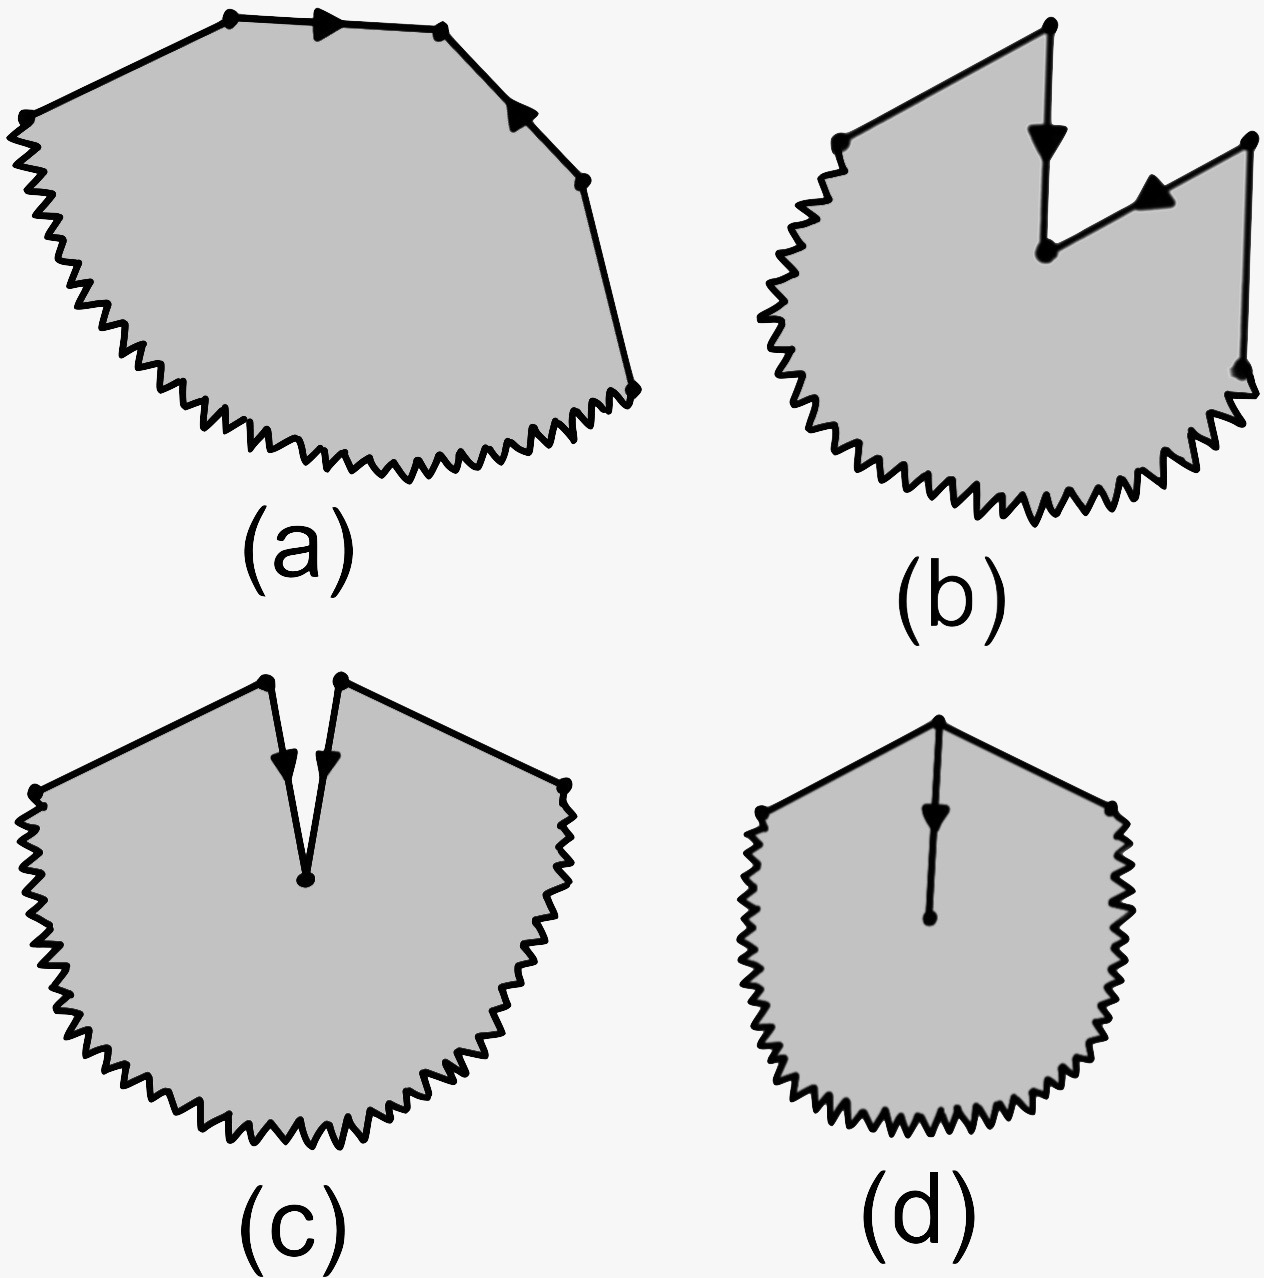
\includegraphics[width=0.4\linewidth]{imagenes/paso2.jpeg}
	\caption{Eliminando adyacencias de primera especie}
	\label{fig:paso2}
\end{figure}

\section{Tercer paso}

En este paso procederemos a transformar el polígono $D$ para que todos sus vértices estén identificados entre sí, es decir, buscamos que todos los vértices representen el mismo punto en la superficie $S$. Partamos del $D$ resultante del paso 2.

Podemos dividir los vértices en clases de equivalencia según qué vértices están identificados. Supongamos que al menos hay dos clases de equivalencias e intentemos eliminar una de ellas.\\
Como hay dos clases de equivalencia, entonces existen al menos dos vértices adyacentes $P$ y $Q$ tal que no pertenecen a la misma clase, ilustramos en la figura \ref{fig:paso3} cómo procederemos. Sabemos que $a$ y $b$ no pueden estar identificados\footnote{No puede ser par de primera especie porque ya hemos aplicado el segundo paso, y no puede ser par de segunda especie porque los vértices son distintos.}, entonces cortamos e identificamos a lo largo de la línea $c$ como muestra la figura. Al finalizar la transformación, tenemos un vértice menos de la clase $P$ y uno más de la clase $Q$. Una vez eliminado el vértice, se aplica el segundo paso nuevamente de ser posible y se repite el procedimiento. Tras un número finito de pasos habremos eliminado la clase de equivalencia de $P$. Iteramos de forma análoga hasta que tengamos una única clase de equivalencia de vértices del polígono.

\begin{figure}[h!]
	\centering
	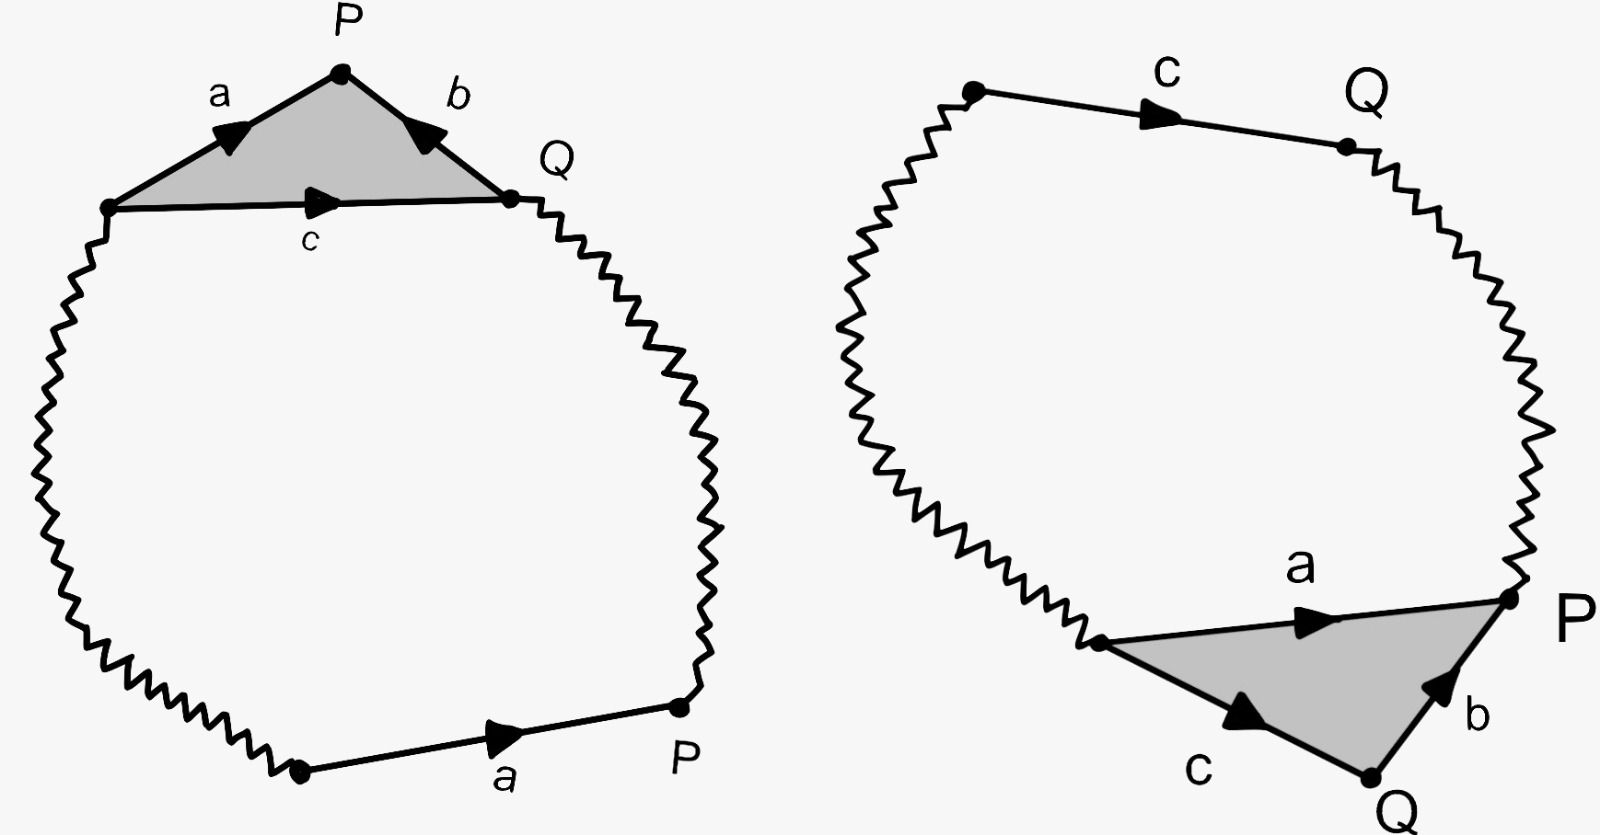
\includegraphics[width=0.4\linewidth]{imagenes/paso3.jpeg}
	\caption{Reduciendo clases de equivalencia de vértices}
	\label{fig:paso3}
\end{figure}


\section{Cuarto paso}

Ahora buscaremos hacer adyacentes todos los pares de aristas de segunda especie.

En la figura \ref{fig:paso4} ilustramos el proceso. Partimos de que tenemos dos aristas $b$ de segunda especie no adyacentes, y procedemos a cortar e identificar a través de $a$. Como resultado hemos cambiado un par no adyacente a uno adyacente. Repetimos el mismo procedimiento hasta que todas las aristas de segunda especie sean adyacentes.

\begin{figure}[h!]
	\centering
	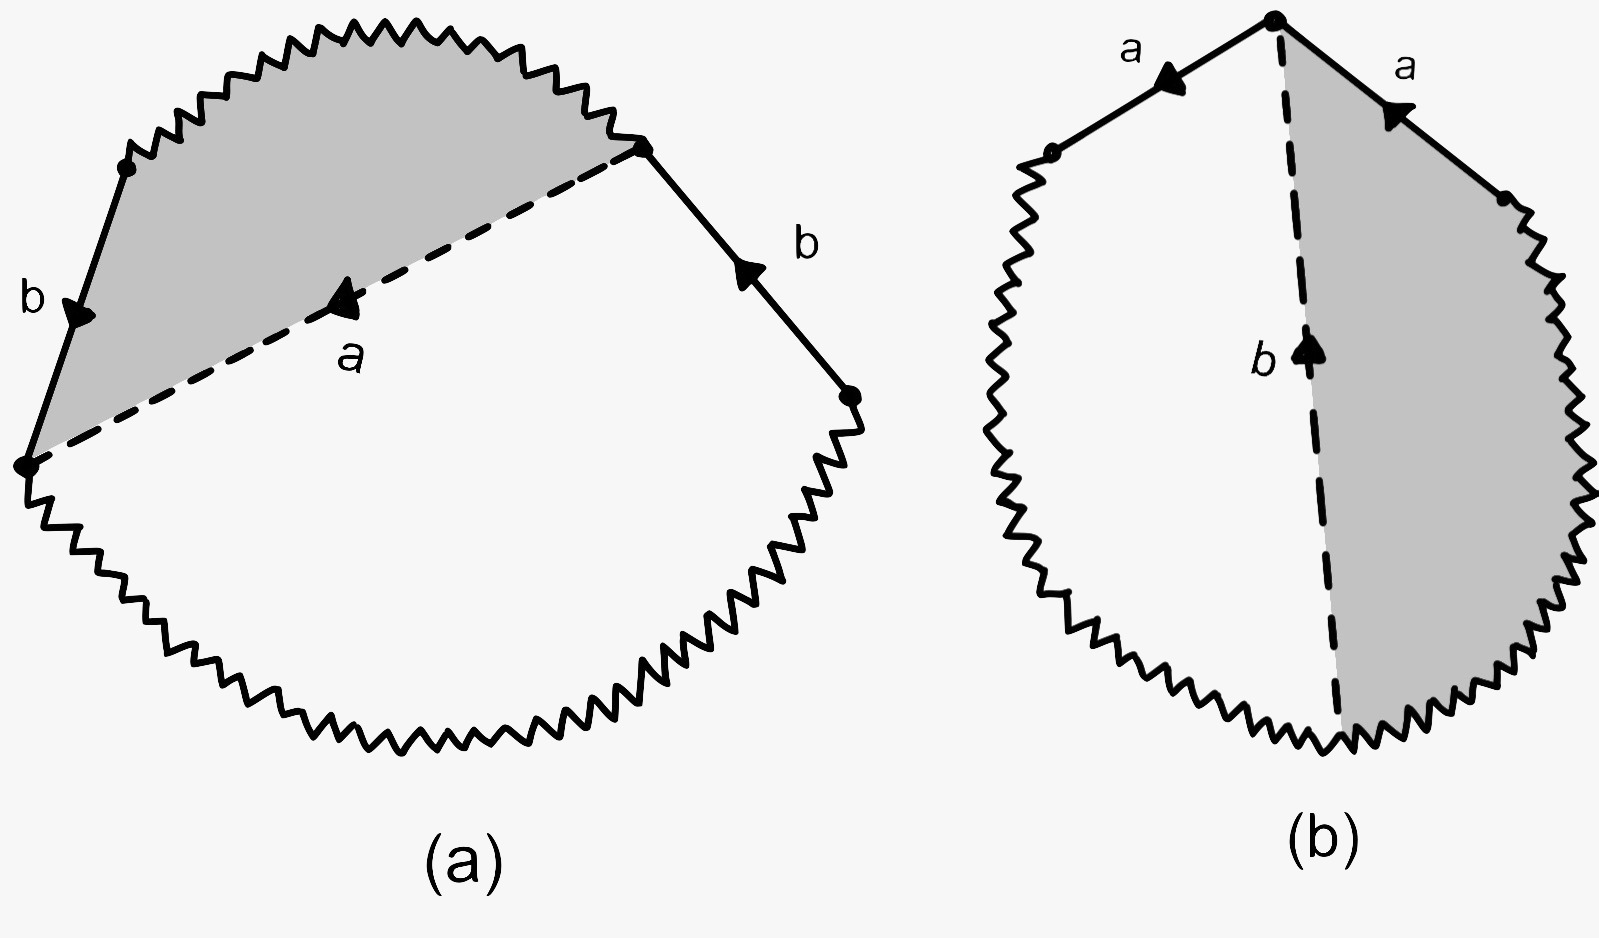
\includegraphics[width=0.4\linewidth]{imagenes/paso4.jpeg}
	\caption{Transformando en adyacentes aristas de segunda especie}
	\label{fig:paso4}
\end{figure}

En caso de no haber ninguna arista de primera especia, entonces tendremos unas expresión de la forma $a_1a_1a_2a_2...a_na_n$, con lo que concluimos que la superficies es homeomorfa a la suma conexa de $n$ planos proyectivos (véase \ref{subsec:expresionescanonicassumasconexas}).

En caso de haber un par de  aristas de primera especie, denotémosla por $c$, probaremos que necesariamente existe otro par de primera especie que las intercala. En otras palabras, necesariamente existe otro par de aristas de primera especie, $d$, tal que la expresión obtenida es de la forma $c...d...c^{-1}...d^{-1}...$

\begin{figure}[h!]
	\centering
	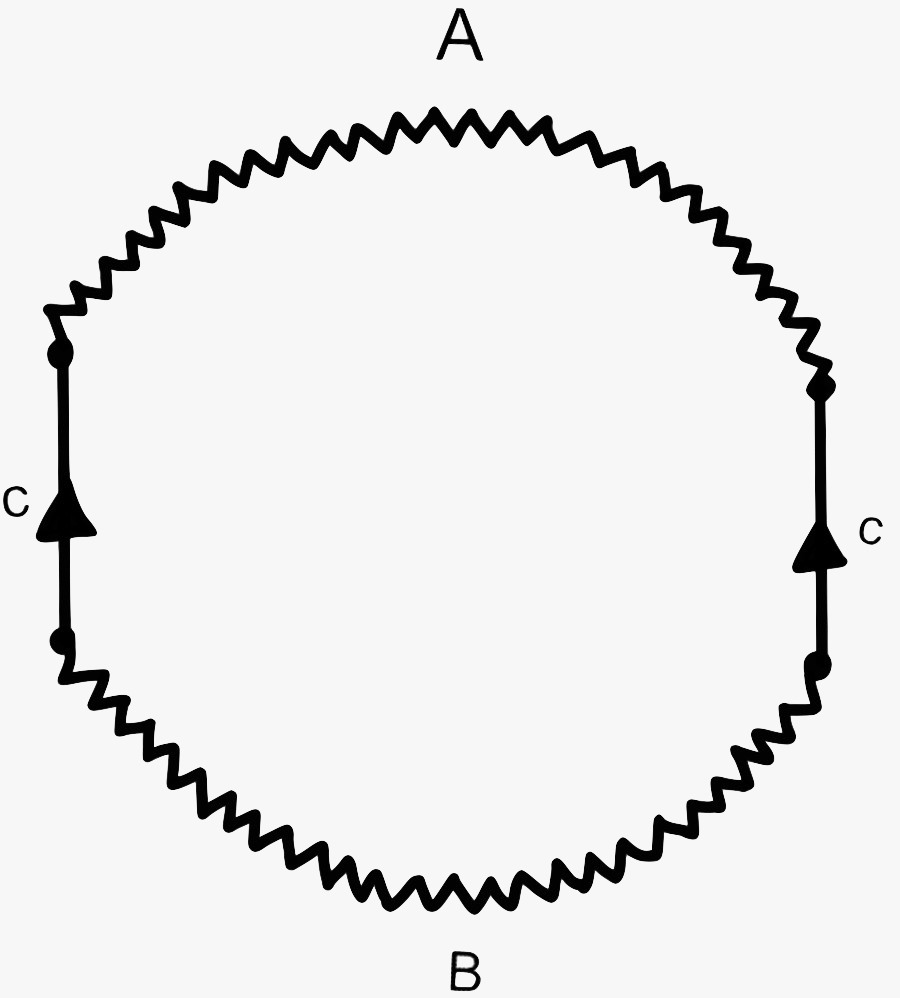
\includegraphics[width=0.2\linewidth]{imagenes/paso4_2.jpeg}
	\caption{Par de primera especie tras el paso 4}
	\label{fig:paso4_2}
\end{figure}

Para probar esto, supongamos que no existe el par $d$. Bajo este supuesto el aspecto del polígono $D$ sería similar a \ref{fig:paso4_2}, donde A y B son ambas sucesiones de aristas. Por el cuarto paso, todas las aristas de segunda especie son adyacentes, con lo que, bajo el supuesto de que no exista $d$, entonces no existiría ninguna arista de A identificada con una de B, ni viceversa. Sin embargo, ello implicaría que los vértices finales e iniciales de la arista $c$ no están identificados\footnote{El lema \ref{lema:lema2detriangulacion} nos permite crear un argumento por contradicción: Si hubiera algún vértice identificado en A y B, entonces podríamos identificar un par de aristas de este vértice entre sendas sucesiones (pero esto no ocurre por hipótesis).}, con lo que incurrimos en una contradicción con el tercer paso.


\section{Quinto paso}

En este paso haremos adyacentes los pares de aristas de primera especie que estén intercalados como se indica en el paso anterior.

Supongamos que nuestro polígono tiene la expresión $a \ldots b \ldots a^{-1} \ldots b^{-1}$ (véase la figura \ref{fig:paso5} $(a)$). Primero, cortamos a lo largo de $c$ y pegamos las aristas $b$, obteniendo la figura \ref{fig:paso5} $(b)$.  Seguidamente, cortamos a lo largo de $d$ y pegamos $c$, con lo que obtenemos la figura \ref{fig:paso5} $(c)$. Nótese que hemos transformado nuestra expresión cambiando los pares $a$ y $b$, por $cdc^{-1}d^{-1}$.  De los pasos se sigue que los vértices siguen manteniendo una única clase de equivalencia.

\begin{figure}[h!]
	\centering
	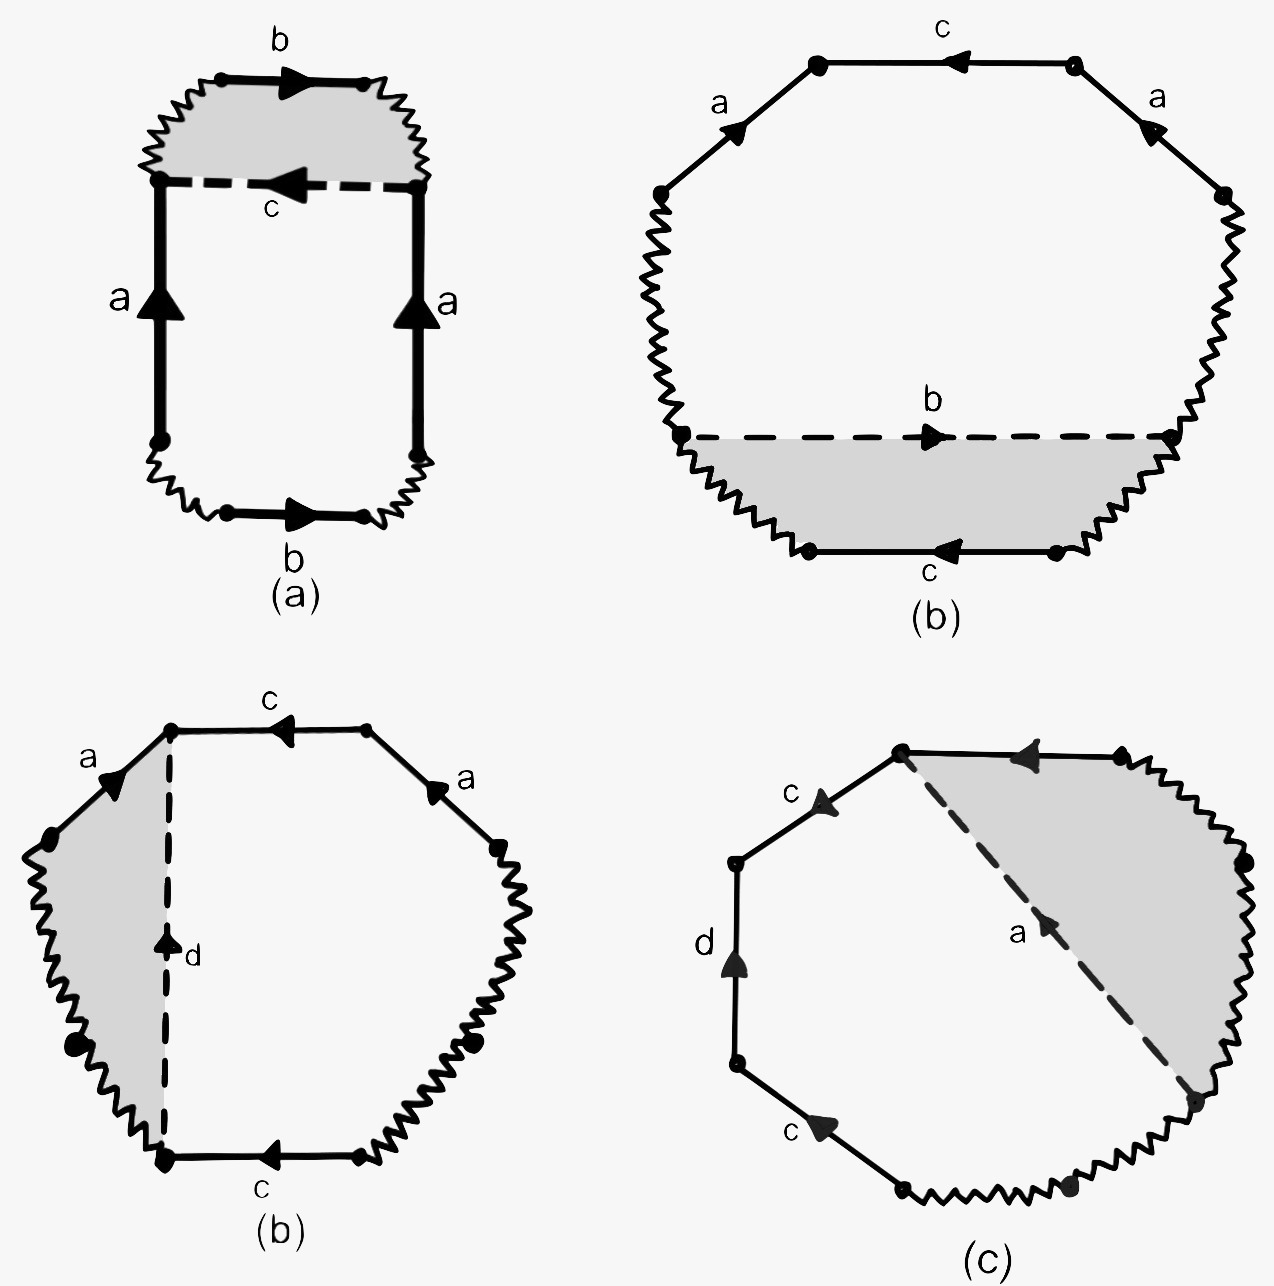
\includegraphics[width=0.4\linewidth]{imagenes/paso5.jpeg}
	\caption{Haciendo adyacentes pares de primera especie intercalados.}
	\label{fig:paso5}
\end{figure}

Repetimos el mismo procedimiento hasta que todos los pares de aristas de primera especie estén agrupados de la forma  $cdc^{-1}d^{-1}$. Si no hay pares de arista de segunda especie, la expresión sería 
\[a_1 b_1 a_1^{-1} b_1^{-1} a_2 b_2 a_2^{-1} b_2^{-1} \ldots a_n b_n a_n^{-1} b_n^{-1}\]
con lo que la superficie es equivalente a una suma conexa de $n$ toros (véase la sección \ref{subsec:expresionescanonicassumasconexas}).


\section{Desenlace final}

Tras los cinco pasos anteriores hemos tenido en cuenta los casos en los que la superficie es homeomorfa a una esfera, una suma conexa de $n$ planos proyectivos o una suma conexa de $m$ toros. Consideremos ahora el caso en el que la expresión tiene tanto aristas de segunda especie (adyacentes), como aristas de primera especie (agrupadas en conjuntos de cuatro). La expresión de este último caso corresponde con una suma conexa de $n$ toros y $m$ planos proyectivos:
\[ a_1 b_1 a_1^{-1} b_1^{-1} \ldots a_n b_n a_n^{-1} b_n^{-1} c_1 c_1 \ldots c_m c_m \] 

Utilizando el lema \ref{lema:planop+toro=3planop} en el anexo, tenemos que cada suma de toro más plano proyectivo puede sustituirse por la suma conexa de tres planos proyectivos. Luego del lema se sigue que, en este último caso, nuestra superficie corresponde con una suma conexa de $m+2n$ planos proyectivos, con lo que queda demostrado el teorema.

En virtud de lo mencionado sobre orientabilidad en la sección \ref{sec:orientabilidad}, podemos reformular el teorema de clasificación como:

\begin{teorsin}
Toda superficie compacta orientable es topológicamente equivalente a una esfera o una suma conexa de $n$ toros. Toda superficie compacta no orientable es homeomorfa a una suma conexa de $n$ planos proyectivos.
\end{teorsin}

Definimos entonces el \textbf{género} de una superficie compacta como el valor de $n$ que le corresponde por homeomorfismo en el teorema anterior. En caso de que la superficie sea homeomorfa a una esfera diremos que tiene género 0. \\
Para probar que el género está bien definido hace falta demostrar que las clases de equivalencia mencionadas no son homeomorfas entre sí. Una prueba se construye en \cite{massey} utilizando la relación \ref{gen_carE} entre el género ($g$) y la característica de Euler ($x$), y demostrando la invariancia topológica de la característica.
\begin{equation}
\label{gen_carE}
g = \begin{cases}
\frac{1}{2}(2-x) & \quad \text{si la superficie es orientable}\\
2-x & \quad \text{si la superficie no es orientable}
\end{cases}
\end{equation}

\section{Superficies con borde y su clasificación}
\label{sec:superfborde}
La noción de superficie con la que hemos trabajado hasta ahora no contempla `bordes'. Por ejemplo, si tomamos el cuadrado cerrado
\[
C = \{(x,y)\in \reales^2:\; 0 \leq x \leq 1, \: 0 \leq y \leq 1  \}
\]
comprobamos que no satisface la definición \ref{defin:superficie}: el punto $(0,0)$ no tiene ningún entorno homeomorfo a $U^2$. Ampliamos entonces el concepto de superficie:

\begin{defin}
Diremos que un espacio topológico $S$ es una \textbf{superficie con borde} si cumple ser conexo, Hausdorff y segundo numerable. Donde, además, se cumple que todo punto en $S$ tiene un entorno homeomorfo a $U^2$ o a
\[H^2 = \{(x,y)\in U^2:\; y\geq0 \}\]
Llamaremos \textbf{borde} de la superficie al conjunto de puntos que tienen entornos homeomorfos a $H^2$, e \textbf{interior} de la superficie al conjunto de puntos con entornos homeomorfos $U^2$.
\end{defin}

Utilizando el teorema \ref{teor:teoremadeclasificacion} y un razonamiento similar al de su demostración, se puede probar la clasificación para las superficies con borde:

\begin{teor}
Dos superficies con borde compactas son homeomorfas si y solo si tienen el mismo número de componentes de borde, son ambas orientables o ambas no orientables, y tienen la misma característica de Euler.
\end{teor}

Una demostración rigurosa se puede leer en \cite{massey}. Equivalentemente, podemos enunciar el teorema como: Toda superficie con $k$ componentes de borde es homeomorfa a una esfera, o a una suma conexa de $n$ toros o a una suma conexa de $n$ planos proyectivos, en los cuales retiramos $k$ discos abiertos. Este enunciado alternativo nos permite hablar de género también para el caso de las superficies con borde. 

Con esto cerramos finalmente la clasificación para superficies compactas y  podemos sumergirnos en el mundo más variado de la no compacidad!



\chapter{Hacia las superficies no compactas}

En este capítulo extenderemos la clasificación a superficies no compactas y construiremos una superficie representante para cada clase de equivalencia.\\
El teorema de clasificación de Kerékjártó se basará en la clasificación de superficies compactas con borde estudiada en el capítulo anterior, y en el concepto de ``frontera ideal''. La ``frontera ideal'' será un espacio topológico definido a partir de una superficie dada, que describe el comportamiento de subsuperficies compactas encajadas. Comprobaremos que este espacio topólogico será un invariante que cumplirá también ser totalmente inconexo, separable y compacto. Finalmente, el teorema nos garantizará que, fijado el género y la ``clase de orientabilidad'', dos superficies son homeomorfas si y solo si sus ``fronteras ideales'' también lo son.\\
Las propiedades topológicas de la ``frontera ideal'' nos permitirá formular una especie de recíproco. Veremos que todo espacio totalmente inconexo, separable y compacto es homeomorfo a la frontera ideal de una superficie. Para esta comprobación utilizaremos que todo espacio de dichas propiedades es homeomorfo a un subconjutno del conjunto de Cantor, y partiendo de este conjunto dentro del plano construiremos la superficie adecuada. 
[IMAGEN DE SUPERFICIE NO COMPACTA DE GÉNERO INFINITO)

\section{Definiciones básicas}
Introducimos algunas definiciones que serán útiles para el manejo de las superficies no compactas.

\begin{defin}
Diremos que un subconjunto de una superficie $S$ es \textbf{acotado} si su cierre es comapcto en $S$.
\end{defin}

\begin{defin}
Llamaremos \textbf{subsuperficie} de una superficie dada $S$ a todo subconjunto que cumpla ser una superficie con borde.
\end{defin} 

Recordemos que las superficies tratadas en este trabajo satisfacen por definición ser segundo numerables (por tanto, separables) y que el teorema \ref{teor:teoremaDeTriangulacion} nos sigue garantizando que las superficies estudiadas son triangulables.\\

(REESCRIBIR TODO ESTO DEL GÉNERO Y CEÑIRTE A LAS DEFINICIONES DEL PAPER!!)
Podemos también generalizar el concepto de género que dimos ya para superficies compactas. Diremos que una superficie no compacta tiene género $m > 0$ si toda subsuperficie compacta tiene género igual o inferior a $m$ y existe una subsuperficie compacta para que se satisface la igualdad. Si ocurriése que se pueden construir subsuperficies de género arbitrariamente grandes, entonces diremos que la superficie tiene género infinito. 
\begin{defin}
Diremos que una superficie es \textbf{plana} si toda subsuperficie compacta tiene género 0. 
\end{defin}

De manera similar podemos hablar de la orientabilidad en superficies no compactas. Una superficie puede ser orientable o no orientable. 
\begin{defin}
Diremos que una superficie $S$ es \textbf{infinitamente no orientable} si no existe un subconjutno acotado  $A \subset S$ tal que $A\backslash S$ sea orientable. En caso de existir, diremos que $S$ es \textbf{finitamente no orientable}.
\end{defin}
De la definiciones dadas se sigue que toda subsuperficie infinitamente no orientable necesariamente tiene género infinito.
(TODO: Estas definiciones me dejan un poco intranquilo porque no me esto ciñendo al paper, quizás debería)
(HABLAR MEJOR DE LAS CLASES DE ORIENTABILIDAD Y TODO ESOO)
[INTRODUCIR IMAGEN DE SUPERFICIE NO COMPACTA PLANA, DE GÉNERO FINO E INFINITO]
\\

\subsection{La frontera ideal}
La frontera ideal es un espacio topológico que da una descripción de cómo subconjuntos compactos de una superficie separan la superficie en conjuntos no acotados. Se construye como el conjunto de clases de equivalencia de los ``finales'', concepto que definimos a continuación:

\begin{defin}
Un \textbf{final} de una superficie $S$ es una secuencia de conjuntos encajados $P_1 \supset P_2 \supset \ldots$, donde $P_i$ es un conjunto conexo no acotado de $S$ que cumple:
\begin{enumerate}
\item[(a)] La frontera de $P_i$ es compacto para todo $i$;
\item[(b)] Para cualquier subconjunto acotado $A \subset S$, $P_i \bigcap A = \emptyset$ para $i$ suficientemente grande.
\end{enumerate}
\end{defin}
Dados dos finales $P_1 \supset P_2 \supset \ldots$ y $P'_1 \supset P'_2 \supset \ldots$, diremos que son equivalentes si para todo $n$ existe un correspondiente $N$ tal que $P_n \subset P'_N$ y viceversa.  Esta regla establece una relación de equivalencia. Denotaremos por $p*$ a la clase de equivalencia del final $p = P_1 \supset P_2 \supset \ldots$.

\begin{defin}
La \textbf{frontera ideal} de una superficie $S$ es el espacio topológico $B(S)$ que tiene por elementos las clases de equivalencia de finales, y tiene por base los conjuntos $U^*$: donde $U\subset S$ es cualquier conjunto  cuya frontera sea compacta; y los elementos de $U*$ son los finales $p*$ que satisfagan que, fijado un representante $p=P_1 \supset P_2 \supset \ldots $, exista un $n$ con $P_n \subset U$.
\end{defin}
Para probar que la frontera ideal está bien definida es preciso comprobar que los elementos de cualquier $U*$ no dependen del representante escogido, esto se sigue directamente de la relación de equivalencia establecida entre finales. Además, es necesario probar que el conjunto propuesto, en efecto, forma una base de una topología, para ello comprobamos que: eligiendo $U=\emptyset$ tenemos el abierto $U^*=B(S)$; tomando $U = S$ tenemos el abierto $U^*=\emptyset$; y, en el siguiente lema, veremos que $U^* \cap V^* = (U \cap V)^*$, que prueba que el conjunto es una base y con ello se demuetra que el espacio $B(S)$ está bien definido.

\begin{lema}
Dada una superficie $S$ y dos conjuntos  con frontera compacta $U,V \subset S$, entonces se cumple que $U^*\cap V^* = (U \cap V)^* $.
\end{lema}
\begin{proof}
Primero veamos que $U^*\cap V^* \supset (U \cap V)^* $:
\[
p^* \in (U \cap V)^* \Rightarrow
\exists n \quad p_n \subset (U \cap V) \Rightarrow
p^* \in U, \: p^* \in V
\]
Por otra parte, veamos $U^*\cap V^* \subset (U \cap V)^* $:
\begin{align*}
p^* \in U, \: p^* \in V & \Rightarrow \exists n,m \quad p_n \subset U, \: p_m \subset V\\
& \Rightarrow n' = \max(n,m), \; p_{n'} \subset U \cap V\\
& \Rightarrow p^* \in (U\cap V)^*
\end{align*}
\end{proof}

Del mismo modo conviene demostrar la misma propiedad para la unión:
\begin{lema}
Dada una superficie $S$ y dos conjuntos  con frontera compacta $U,V \subset S$, entonces se cumple que $U^*\cup V^* = (U \cup V)^* $.
\begin{proof}
Si $U$ y $V$ tienen frontera compacta entonces $U\cup V$ también. El siguiente razonamiento comprueba $U^*\cup V^* \subset (U \cup V)^* $:
\[
q^* \in U^*\cup V^* \Rightarrow 
\exists n \: q_n \subset U \: \vee \: q_n \subset V \Rightarrow
\exists n \: q_n \subset U \cup V \Rightarrow
q^* \in (U \cup V)^*
\]
El otro contenido lo comprobaremos por contradicción. Supongamos que $q^* \in (U \cup V)^*$, pero que para todo $n$ tenemos que $q_n \nsubseteq U$ y $q_n \nsubseteq V$. Como la frontera de $U \cup V$ y la de $V^c$ son compactas, podemos elegir un $n$ tal que $fr(V^c)\cap q_n = \emptyset$ y que $q_n \subset Int(U\cup V)$. Entonces podemos proponer  la partición de $q_n$ en los abiertos $Int(V) \cap Int(U \cup V)$ e  $Int(V^c) \cap Int(U \cup V)$, disjuntos y ambos con intersección con $q_n$ no vacía por la hipótesis inicial; sin embargo, esto contradice que $q_n$ sea conexo.
\end{proof}
\end{lema}

\begin{defin}
Sea $p^*$ el representante de un final $p =P_1 \supset P_2 \supset \ldots$, diremos que $p^*$ es \textbf{plano/orientable} si existe un $N$ tal que para todo $n>N$ los conjuntos $P_n$ son superficies planas/orientables.
\end{defin}

La definición anterior nos permite considerar los conjuntos $B(S) \supset B'(S) \supset B"(S)$, donde $B'(S)$  es el conjunto de los finales no planos y $B"(S)$ es el conjunto de los finales no orientables. A partir de ahora consideraremos la frontera ideal como la terna $(B(S), B'(S), B"(S))$.
\begin{lema}
Los conjuntos $B'(S)$ y $B"(S)$ son cerrados. 
\end{lema}
\begin{proof}
Veamos que $A = (B'(S))^c$ es un abierto:\\
Sea $p^* \in A$ entonces existe un $n$ con $P_n$ plano. Definimos el conjunto:
\[
C = \bigcup_{p^* \in A} Int(P_n)^*
\]
$C$ es abierto por ser unión de abiertos. Bastaría con ver que $C=A$: por un lado, se sigue de la definición que $A\subset C$; por otro, si $q^* \in C$ entonces existe un $n$ y un $m$ con $q_m \subset Int(P_n)$, como $P_n$ es plano entonces $q_m$ también, con lo que concluimos que $q^* \in A \Rightarrow C\subset A$.\\
Una demostración totalmente análoga comprueba que $B = (B"(S))^c$ es abierto.
\end{proof}

\textbf{Ejemplo:} Si para todo subconjunto compacto $A\subset S$, se tiene que $S\backslash A$ tiene como mucho $m$ componentes no acotadas, y se cumple que para algún $A$ el valor es exactamente $m$, entonces el conjunto $B(S)$ consiste de $m$ clases de equivalencia de finales (donde cada uno puede ser plano, orientable y no plano, o no orientable). Si $m=0$ tenemos una superficie compacta.

[EJEMPLO CON M=4]

El siguiente par de propiedades son herramienta utilizadas por el teorema de Kerékjárto:

\begin{lema}
Sea $S_1$ una subsuperficie de $S$, tendremos que $S_1^* \in B(S)$ un final no plano/no orientable si y solo si $S_1$ es de género infinito/es infinitamente no orientable. De la misma forma, $S_1^*$ es no vacío si y solo si $S_1$ es no acotado.
\end{lema}

\begin{lema}
\label{lema:fronteraidealnoconexo}
La frontera ideal de una superficie separable es un espacio totalmente inconexo, separable y compacto.
\end{lema}
Una demostración rigurosa de este hecho se da en [AGREGAR REFERENCIA, SALE EN EL PAPER].

\section{Teorema de Kerékjárto}
\begin{teor}
Sean $S$ y $S'$ dos superficies separables del mismo género y clase de orientabilidad. Entonces $S$ y $S'$ son homeomorfa si y solo si las fronteras ideales (como ternas de espacios) son homeomorfas.
\end{teor}

\subsection{Idea de la demostración}
La demostración sigue un razonamiento inductivo, para demostrarlo son necesarios varios pasos técnicos. En el trabajo daremos una idea de la demostración sin detenernos a analizar esos detalles.

[AGREGAR DEMOSTRACIÓN]

\section{Construcción de una superficie con frontera ideal dada}
Recordemos que la proposición \ref{lema:fronteraidealnoconexo} nos garantiza que la frontera ideal es un espacio espacio totalmente inconexo, separable y compacto. Demostraremos ahora que para cualquier terna de espacios topológicos $X \supset Y \supset Z$, con $Y$ y $Z$ cerrados de $X$, que cumplan dichas propiedades, son homeomorfos a la frontera ideal de alguna superficie. Ian Richards en [AGREGAR REFERENCIA] construye la superficie que da demostración a este hecho. \\

\begin{lema}
\label{lema:cantor}
Cualquier espacio compacto, totalmente inconexo y separable es homeomorfo a un subconjunto del conjunto de Cantor.
\end{lema}
[Agregar referencia donde se demuestre?]

Con este resultado podemos proceder a enunciar y demostrar el teorema de Ian Richards:

\begin{teor}
Sea $(X,Y,Z)$ una terna cualquiera de espacios compactos, separables y totalmente inconexos con $Z \subset Y \subset X$.  Entonces existe una superficie $S$ cuya frontera ideal es $(B(S), B'(S), B"(S))$ que es topológicamente equivalente a $(X,Y,Z)$
\end{teor}

\subsubsection*{Idea de la demostración}
La construcción partirá de una esfera a la cual retiraremos un conjunto de puntos y discos abiertos, cada punto representará un final y los discos serán convenientemente identificados para crear  subsuperficies de género 1 (o bien un toro o bien un plano proyectivo). Configurando adecuadamente estos dos elementos conseguiremos una frontera ideal homeomorfa a $(X,Y,Z)$.\\
Procederemos primero construyendo la superficie y luego comprobando que cumple la condición especificada.


\subsubsection*{Demostración}
Por el lema \ref{lema:cantor} podemos asumir que $X$ es un subconjunto del conjunto de Cantor, el cual consideramos inmerso en el plano compactificado (homeomorfo a la esfera) como el conjunto de puntos $(x,0)$ con $0 \leq x\leq 1$ donde $x$ tiene una expresión triádica sin el dígito 1.

[IMAGEN DE TAL CONJUNTO DE CANTOR]

Elegimos $D'$ el conjunto de todos los discos cerrados del plano que tienen por diámetro los intervalos $[\frac{n - 1/3}{3^m} , \frac{n + 4/3}{3^m} ] x {0}$ , con $0\leq n \leq 3^m$, donde $n$ es un entero que admite una expresión triádica sin el dígito 1. Sea $D$ el subconjunto de discos de $D'$ que contienen al menos un punto de $X$.\\

[IMAGEN DEL CONJUNTO D Y X]

Los discos de $D$ intersecados con $X$ determinan una base de la topología de $X$. Los discos de $D$ cumplen las siguientes dos propiedades:
\begin{enumerate}
\item Cuales quiera dos discos del conjunto son o bien disjuntos o bien uno está contenido dentro del otro (véase [REFERENCIA A IMAGEN]).
\item Si tenemos una cadena de discos $D_1 \supset D_2 \supset \ldots$, entonces la intersección de todos esos discos  con el eje x es un único punto de $X$ (este hecho se comprueba viendo que podemos excluir cualquier otro punto de la intersección). Más aún, se tiene que el conjunto de discos de $D$ que contienen a un $x \in X$ se pueden representar como una secuencia $D_1 \supset D_2 \supset \ldots$ cuya intersección es $x$.
\end{enumerate}
Sea $P^+$ y $P^-$ los planos $y > 0 $ e $y < 0$, respectivamente. Para cada disco $K$ en $D$, denotamos por $K'$ y por $K"$ los dos discos más grandes contenidos propiamente en $K$ (Cualquier otro disco propiamente contenido en $K$ estará por tanto contenido o en $K'$ o en $K"$, véase la figura [AGREGAR REFERENCIA]).
[FIGURA CON K' Y K "]

Ahora, para cada disco $K$ en $D$ elegimos dos discos abiertos $C^+(K)$ y $C^-(K)$, cada uno contenido en $K$  y que satisfagan:
\begin{enumerate}
\item[(a)] $C^+(K) \subset P^+$ y $C^-(K) \subset P^-$
\item[(b)] $C^+(K)$ y $C^-(K)$ no intersequen ni a $K'$ ni a $K"$.
\item[(c)] $C^+(K)$ y $C^-(K)$ son simétricos respecto al eje x.
\end{enumerate}
Con lo que ningunos dos círculos $C^\pm(K)$ se intersecan entre sí.
[IMAGEN DE CÓMO SERÍAN ESTOS DISCOS]
Construimos nuestra superficie $S$ como la esfera homeormofa al plano compactificado en el que retiramos los puntos de $X$ y algunos de los círculos $C^\pm(K)$. Primero, retiramos los círculos $C^\pm(K)$ que están dentro de un $K\in D$ con $K \cap Y \neq \emptyset$, si por el contrario  $K \cap Y = \emptyset$, entonces ignoramos los círculo. El segundo caso corresponderá con los finales planos. Luego,  si ocurre que $K \cap Y \neq \emptyset$  y $K \cap Z = \emptyset$, entonces identificamos $C^+(K)$ con $C^-(K)$ reflejando el primero en el eje x (preservando la orientación), estos corresponderán con los finales de género infinito orientables.  Por último, si $K \cap Z \neq \emptyset$, entonces identificamos los círculos por traslación (invirtiendo la orientación), en cuyo caso tendremos finales de género infinito no orientables.\\
Queda ahora probar que la $S$ que se obtiene tiene una frontera ideal equivalente a la terna $(X,Y,Z)$. (AQUÍ HAY QUE METERSE EN TECNISISMOS, terminar).



\subsection{Construcción de superficie no compacta de género finito}
[TODO]
\subsubsection*{Numerabilidad de las clasificaciones}
[TODO]




\chapter{Anexo: Algunos resultados que utilizamos en el trabajo}

\begin{lema}\label{lema:sumaconexa}
	Para verificar que la suma conexa está bien definida hace falta aclarar varios puntos.
	\begin{enumerate}
		\item 
		Tenemos que asegurar la existencia de un subconjunto homeomorfo a un disco.
		\begin{proof}
			Tomamos un punto $p\in S_i$ cualquiera. Como $S_i$ es una 2-variedad, entonces existe un homeomorfismos $g$ que manda un entorno, $U$, del punto $p$ al círculo abierto. 
			
			Tomamos $E_{\frac{1}{2}}$ el disco cerrado de radio $\frac{1}{2}$, y $U'= g^{-1}(E_{\frac{1}{2}})$. Tenemos que $g\mid_{U'}$ es un homeomorfismo de un subconjunto de $S_i$ a $E_{\frac{1}{2}}$ que a su vez es homeomorfo al disco cerrado de radio 1. 
		\end{proof} 
		\item 
		Segundo, tenemos que asegurarnos que existe un tal $\psi$ homeomorfismo:
		\begin{proof}
			Utilizando los $g$ anteriores basta ver que  $g(fr(D_i))=fr(E^2)$, y luego componer las funciones para construir un homeomorfismo entre las fronteras.
		\end{proof}
		\item 
		Tercero, habría que comprobar que, en efecto, el objeto obtenido es una superficie. Es decir, comprobar que todo punto tiene un entorno homeomorfo al disco abierto, que el espacio es T2 y que es conexo.
		\begin{proof}
			Ideas (hace falta formalizarlo?)
			1. Entorno homeomorfo a la bola: Tenemos que comprobarlo para los ptos frontera. Esta dems es engorrosa: Basta quizás con ver que localmente podemos tratar a los puntos de la frontera como si estuviesemos en R2, observando las construccioines de homeomorfismos podemos concluir que se puede crear un entorno homeomorfo a una bola al pegar dos semicírculos de cada superficie (vistas en R2 localmente). 
			2. Conexión: Basta con probar que para todos los puntos del borde  sus abiertos tienen puntos de ambas superficies. Esto se sigue directamente de la topología cociente inducida (analizar la definición con la función cociente, tendrás puntos en ambas superficies por tener abtos en ambas).
			3. Ver que es T2 resulta sencillo. Si los ptos son de superficies distintas, ya está, por ser disjuntas. Si son de la misma entonces también, porque antes eran t2. Si una es de la superficie, por concretar, de S1 y la otra del borde, entonces tomamos los mismos abtos que antes separaban a los puntos, pero el abto del borde ya no es abto de la superficie cociente, es fácil comprobar que ese conjunto unión S2' sí es un abto (por la def de topo cociente, todos los ptos serán interiores) y también es fácil ver que estos dos conjuntos serán disjuntos, por lo que hemos separado los dos ptos.
		\end{proof}
		\item 
		Y, finalmente, tenemos que comprobar que esta definición es independiente de los conjuntos $D_i$ escogidos e independiente de los homeomorfismos.
		\begin{proof}
			Ideas (hace falta formalizarlo?):
			1. Que no depende del homeomorfismo es directo porque solo nos hace falta esa propiedad para establecer la topología cociente. Habiendo probado el punto anterior ya estaría.
			2. Que no depende de la elección del disco se sigue de que podemos desplazar el disco por la superficie manteniendo el homeomorfismo con la superficie anterior. De no poder hacerlo entonces tendríamos que no se puede retirar un disco en la zona a la que estamos desplazándolo, pero en ese caso sencillamente no tomaríamos esa elección de disco por ser imposible.
		\end{proof}
	\end{enumerate} 
\end{lema}


\begin{lema}\label{lema:planop+toro=3planop}
La suma conexa de un toro y un plano proyectivo es homeomorfa a la suma conexa de tres planos proyectivos.
\end{lema}
\begin{proof}
TODO
\end{proof}





\chapter{COSAS QUE NO HE UTILIZADO}

\begin{figure}[h!]
	\centering
	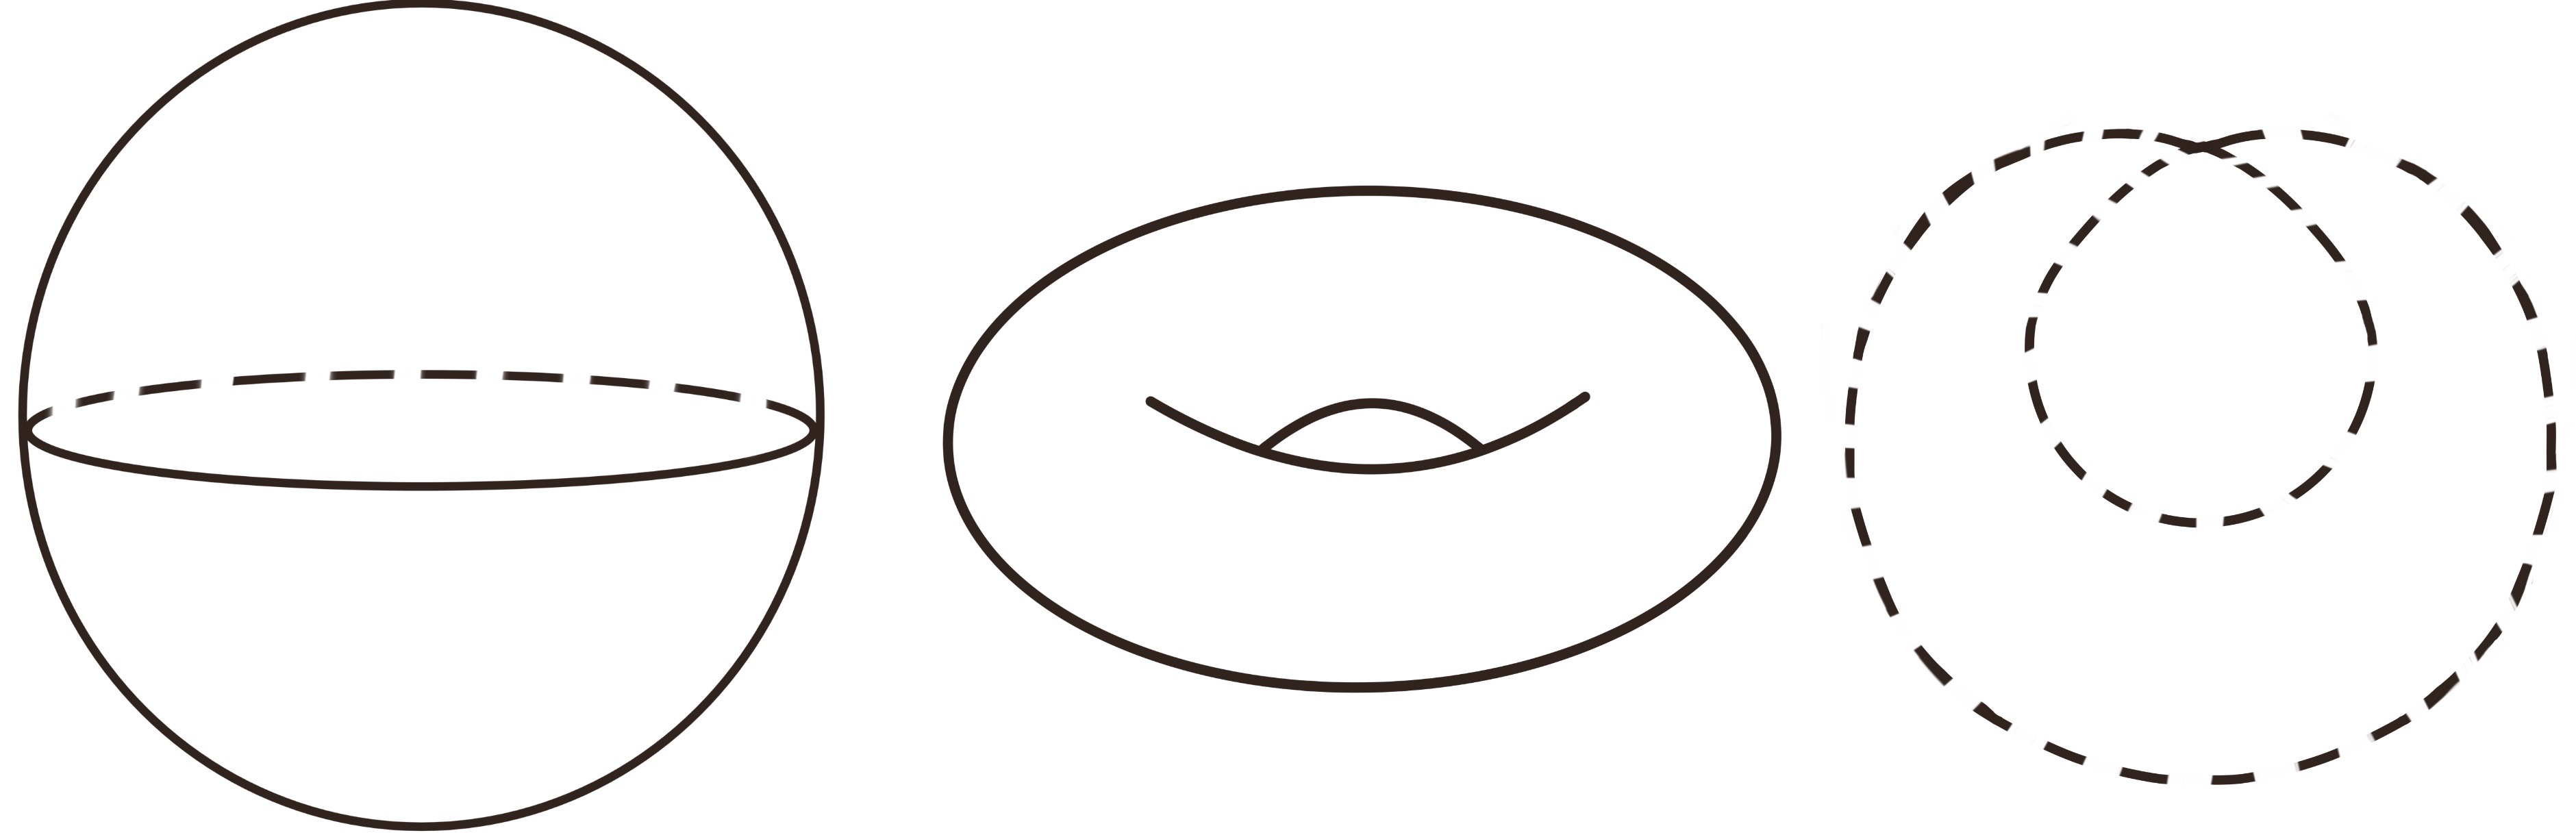
\includegraphics[width=0.5\linewidth]{imagenes/superficies.png}
	\caption{Ejemplos de superficies: Esfera, toro y banda de M\"obius}
	\label{fig:superficies sencillas}
\end{figure} 





\begin{thebibliography}{10}
%% TODO: VER COMO SE TIENEN QUE PONER LAS CITAS
\bibitem{massey} 
    \textsc{William S. Massey}: 
    Introducción a la topología algebraica. 
    \textit{Editorial Reverté} {\bf1} (2006), 1--40.

\bibitem{ian}
    \textsc{Ian Richards}
    \textit{Classification of non compact surfaces...o algo asi}
    
    
\end{thebibliography}
\cleardoublepage
\end{document}
